
% Template based on work by Pedro Tome Gonzalez (2008), thanks a lot for sharing!

%% Los margenes, tipo de hoja y estilo BOOK
\documentclass[a4paper,12pt,twoside,openright,titlepage]{book}
\usepackage[a4paper,left=1.25in,right=1.25in]{geometry}
%\usepackage[a4paper,left=1.5in,right=1in]{geometry} % UNCOMMENT FOR PRINTABLE VERSION (with side margins)
\usepackage[T1]{fontenc}    %Ineterprete de tíldes
%\usepackage[Latin1]{inputenc}
\usepackage{amsmath,amssymb}    %Paquete de entornos matematicos
\usepackage{natbib}
\usepackage[english,spanish]{babel}
\selectlanguage{english} 
\usepackage{graphicx}
\usepackage{psfrag}
\usepackage{quotchap}
\usepackage{epsfig}
\usepackage[all]{xy}

\usepackage[ pdftex, plainpages = false, pdfpagelabels, 
             pdfpagelayout = useoutlines,
             bookmarks,
             hyperfootnotes = false,
             bookmarksopen = true,
             bookmarksnumbered = true,
             breaklinks = true,
             linktocpage,
             pagebackref,
             colorlinks = false,  % was true
             linkcolor = blue,
             urlcolor  = blue,
             citecolor = red,
             anchorcolor = green,
             hyperindex = true,
             hyperfigures
             ]{hyperref} 

\usepackage{epsfig}
\usepackage{makeidx}
\usepackage{ifthen}
\usepackage{multicolpar}    %Para poner texto en columnas en plan articulo intercalado con texto normal
\usepackage{multicol,multirow}

\usepackage{url}        %Para direcciones web
\usepackage{marvosym}   %Para imprimir el simbolo de \EUR euro
%\usepackage{eurosym}   %Para imprimir el simbolo de \euro euro
\usepackage{fancybox}   %Para tablas con bordes redondeados
\usepackage{pdflscape}

\usepackage{setspace}
\usepackage{eurosym}


%% Modificación de la plantilla para adaptarla a los requisitos de PFC
\usepackage{fancyhdr}
\pagestyle{fancy}
%%% Cabeceras y pies de página
\fancyhead[CE,CO]{\emph{Detection and localization of odorants with robots and artificial noses}}
\fancyhead[LE,LO,RE,RO]{}
\fancyfoot[LE,RO]{\thepage}
\fancyfoot[CE,CO]{\leftmark}

\renewcommand{\footrulewidth}{.6pt}


%Definiciones de funciones para los titulos
\newlength\salto
\setlength{\salto}{3.5ex plus 1ex minus .2ex}

\newlength\resalto
\setlength{\resalto}{2.3ex plus.2ex}

\newcommand{\lsection}[1]
                {\section{#1}
                \vskip-.9\resalto   %%%% Aquí reculo el posible salto por defecto de \section
                \hrule
                \vskip+.9\salto}  %%%% vuelvo a realizar el salto (puedes poner otra vez el 90%)


%Para imágenes de entornos estáticos \captionFigure{Texto Caption}{Texto Label}
\newcommand{\captionFigure}[3]{
    \refstepcounter{figure}
    \textbf{Figure \thefigure:} \textbf{#1.} #3 \label{#2}
    \addcontentsline{lof}{section}{\thefigure.\ #1\label{#2}}
}

%Para imágenes de entornos estáticos \NOcaptionFigure{Texto Caption}{Texto Label} "No escribe el caption"
\newcommand{\NOcaptionFigure}[2]{
    \refstepcounter{figure}
    \addcontentsline{lof}{figure}{\thefigure.\ #1\label{#2}}
}


\newcommand{\captionTable}[3]{
    \refstepcounter{table}
    \textbf{Table \thetable:} \textbf{#1.} #3 \label{#2}
    \addcontentsline{lot}{section}{\thetable.\ #1\label{#2}}
}



%% Datos del PFC
\newcommand{\titulo}{Cooperative strategies for the detection and localization of odorants with robots and artificial noses}
\newcommand{\autor}{Carlos Garcia-Saura}
\newcommand{\director}{Nombre Apellido1 Apellido2}
\newcommand{\tutor}{Pablo Varona Martinez}
\newcommand{\vocal}{Nombre Apellido1 Apellido2}
\newcommand{\vocalsup}{Nombre Apellido1 Apellido2}
\newcommand{\presidente}{Nombre Apellido1 Apellido2}
\newcommand{\presidentesup}{Nombre Apellido1 Apellido2}
\newcommand{\fecha}{June 2014}
\newcommand{\carrera}{Degree in Telecommunication Technology and Service Engineering}


\usepackage{graphicx}
\begin{document}

\renewcommand\listtablename{List of Tables}
\renewcommand\listfigurename{List of Figures}
\renewcommand\contentsname{Table of Contents}
\renewcommand\bibname{Bibliography}
\renewcommand\chaptername{Chapter}
\renewcommand\appendixname{Appendix}
\renewcommand\spanishtablename{Table}
%\renewcommand\appendixpagename{Anexos}

\newenvironment{packed_enum}{
\begin{enumerate}
  \setlength{\itemsep}{1pt}
  \setlength{\parskip}{0pt}
  \setlength{\parsep}{0pt}
}{\end{enumerate}}

\newenvironment{packed_itemize}{
\begin{itemize}
  \setlength{\itemsep}{1pt}
  \setlength{\parskip}{0pt}
  \setlength{\parsep}{0pt}
}{\end{itemize}}



\setlength{\baselineskip}{18pt}  %% Espacio interlinea
\setlength{\parskip}{6pt plus 1pt minus 1pt} %% Espacio interpárrafo

\begin{titlepage}
%\setcounter{page}{-1}
\setcounter{page}{0}

\begin{center}

\vspace*{-2.2cm}

\LARGE \textbf{\textsc{Universidad Aut\'onoma de Madrid}}\\

\vspace{.2cm}

\Large \textbf{\textsc{Escuela Polit\'ecnica Superior}}\\

\vspace{0.5cm}

\begin{figure}[h]
    \begin{center}
        \begin{minipage}[c]{0.495\linewidth}
            \rightline{\epsfig{figure=images/logo_eps.eps,width=0.5\linewidth}}
        \end{minipage}
        \begin{minipage}[c]{0.495\linewidth}
            \leftline{\epsfig{figure=images/logo_uam.eps,width=0.5\linewidth}}
        \end{minipage}
    \end{center}
    \label{fig:Escudos}
\end{figure}

%\vspace{0.1cm}

\LARGE \textbf{\textsc{Trabajo de fin de grado}}\\
\normalsize \textsc{\textit{BACHELOR'S THESIS}}\\

\vspace{2.5cm}

\large \MakeUppercase{\textbf{Estrategias cooperativas de detecci\'on y localizaci\'on de olores con robots y narices artificiales}}

\large \MakeUppercase{\textit{\titulo}}

\vspace{2.2cm}

\large{Grado en Ingenier\'ia de Tecnolog\'ias y Servicios de Telecomunicaci\'on}\\
\normalsize\textit{\carrera}

\vspace{1cm}

\Large \textbf\autor \\
\vspace{0.5cm}
%\Large Autor: \textbf\autor \\
\large Tutor: \textbf\tutor \\

\vspace{0.5cm}

\LARGE Junio 2014

\end{center}

\end{titlepage}

\normalsize

\newpage \thispagestyle{empty} % Página vacía
\setcounter{page}{0}




\frontmatter %Define el cuerpo inicial del libro en numeración con letras romanas

\chapter*{}

\vspace*{-2cm}

\begin{center}

\large \MakeUppercase{\textbf{\titulo}}

\normalsize \MakeUppercase{\textit{Estrategias cooperativas de detecci\'on y localizaci\'on de olores con robots y narices artificiales}}

\vspace{2cm}

\Large Author: \textbf{\autor} \\
\Large Tutor: \textbf{\tutor} \\

\vspace{6cm}


Grupo de Neurocomputaci\'on Biol\'ogica \\
\url{http://www.ii.uam.es/~gnb/} \\
%Dpto. de Ingenier\'ia Inform\'atica \\
\vspace{0.1cm}
Escuela Polit\'ecnica Superior \\
Universidad Aut\'onoma de Madrid \\
\vspace{0.5cm}
\Large \fecha

\end{center}

\normalsize

\newpage \thispagestyle{empty} % Página vacía


%\onehalfspacing
%\vspace*{-2cm}
\chapter*{Resumen}
\vspace*{-1.5cm}





En este trabajo de investigaci\'{o}n se aborda el dise\~{n}o de una plataforma rob\'{o}tica orientada a la implementaci\'{o}n de estrategias de b\'{u}squeda cooperativa bio-inspiradas. En particular, tanto el proceso de dise\~{n}o de la parte electr\'{o}nica como hardware se han enfocado hacia la validaci\'{o}n en entornos reales de algoritmos capaces de afrontar problemas de b\'{u}squeda con incertidumbre, como lo es la b\'{u}squeda de fuentes de olor que presentan variaci\'{o}n espacial y temporal. Este tipo de problemas pueden ser resueltos de forma m\'{a}s eficiente con el empleo de enjambres con una cantidad razonable de robots, y por tanto la plataforma ha sido desarrollada utilizando componentes de bajo coste.
Esto ha sido posible por la combinaci\'{o}n de elementos estandarizados -como la placa controladora Arduino y otros sensores integrados- con piezas que pueden ser fabricadas mediante una impresora 3D atendiendo a la filosof\'{i}a del hardware libre (open-source).


Entre los requisitos de dise\~{n}o se encuentran adem\'{a}s la eficiencia energ\'{e}tica -para maximizar el tiempo de funcionamiento de los robots-, su capacidad de posicionamiento en el entorno de b\'{u}squeda, y la integraci\'{o}n multisensorial -con la inclusi\'{o}n de una nariz electr\'{o}nica, sensores de luminosidad, distancia, humedad y temperatura, as\'{i} como una br\'{u}jula digital-.
Tambi\'{e}n se aborda el uso de una estrategia de comunicaci\'{o}n adecuada basada en ZigBee.
El sistema desarrollado, denominado GNBot, se ha validado tanto en los aspectos de eficiencia energ\'{e}tica como en sus capacidades combinadas de posicionamiento espacial y de detecci\'{o}n de fuentes de olor basadas en disoluciones de etanol.

La plataforma presentada -formada por el GNBot, su placa electr\'{o}nica GNBoard y la capa de abstracci\'{o}n software realizada en Python- simplificar\'{a} por tanto el proceso de implementaci\'{o}n y evaluaci\'{o}n de diversas estrategias de detecci\'{o}n, b\'{u}squeda y monitorizaci\'{o}n de odorantes, con la estandarizaci\'{o}n de enjambres de robots provistos de narices artificiales y otros sensores multimodales.


\vspace*{-0.2cm}
\section*{Palabras Clave}
\vspace*{-0.2cm}
Plataforma rob\'{o}tica, b\'{u}squeda de olores, robots cooperativos, estrategias de localizaci\'{o}n, nariz electr\'{o}nica, fuentes de olor, rob\'{o}tica de enjambres, bio-inspiraci\'{o}n, vuelos de L\'{e}vy, Python, hardware libre, printbots, impresi\'{o}n 3D, ZigBee, comunicaci\'{o}n a distancia, OpenCV, visi\'{o}n por ordenador, localizaci\'{o}n de robots

%-------------------------------------------------------------
%\begin{center}
%\line(1,0){250}
%\end{center}
%\vspace*{-2cm}
\chapter*{Abstract}
\vspace*{-1cm}










This research work addresses the design of a robotic platform oriented towards the implementation of bio-inspired cooperative search strategies.
In particular, the design processes of both the electronics and hardware have been focused towards the real-world validation of algorithms that are capable of tackling search problems that have uncertainty, such as the search of odor sources that have spatio-temporal variability.
These kind of problems can be solved more efficiently with the use of swarms formed by a considerable amount of robots, and thus the proposed platform makes use of low cost components.
This has been possible with the combination of standardized elements -as the Arduino controller board and other integrated sensors- with custom parts that can be manufactured with a 3D printer attending to the open-source hardware philosophy.

Among the design requirements is the energy efficiency -in order to maximize the working range of the robots-, their positioning capability within the search environment, and multiple sensor integration -with the incorporation of an artificial nose, luminosity, distance, humidity and temperature sensors, as well as an electronic compass-.
Another subject that is tackled is the use of an efficient wireless communication strategy based on ZigBee.
The developed system, named GNBot, has also been validated in the aspects of energy efficiency and for its combined capabilities for autonomous spatial positioning and detection of ethanol-based odor sources.

The presented platform -formed by the GNBot, the GNBoard electronics and the abstraction layer built in Python- will thus simplify the processes of implementation and evaluation of various strategies for the detection, search and monitoring of odorants with conveniently standardized robot swarms provided with artificial noses and other multimodal sensors.

\vspace*{-0.2cm}
\section*{Keywords}
\vspace*{-0.2cm}
Robotic platform, olfactory search, cooperative robots, search strategies, machine olfaction, odor sources, swarm robotics, bio-inspiration, L\'{e}vy walks, Python, open-source hardware, printbots, 3D-printing, ZigBee, remote communications, OpenCV, computer vision, localization of robots



\onehalfspacing
\chapter*{Acknowledgements}
\vspace{-1cm}

This project is the milestone that represents the successful completion of my \emph{Degree in Telecommunication Technology and Service Engineering} at \emph{Universidad Aut\'{o}noma de Madrid}.

My four years as a student at \emph{Escuela Polit\'{e}cnica Superior}\footnote{\url{http://www.eps.uam.es/}} have given me the chance to meet very interesting people, at both a personal and professional level. All of my friends and family have been very kind and supportive from the beginning of this period, and our professors have always contributed to the highest degree of excellence in our studies.
Without all of you I surely would not be where I am sitting today.

I also want to express my most sincere gratitude to all the members at \emph{Grupo de Neurocomputaci\'{o}n Biol\'{o}gica}\footnote{\url{http://www.ii.uam.es/~gnb/}}, and in particular to my tutors \emph{Dr Pablo Varona Mart\'{i}nez} and \emph{Dr Francisco de Borja Rodr\'{i}guez}. Your excellence in research is a reference to me, and your enthusiastic guidance and constant support have been essential towards the success of this project.

Finally, I want to acknowledge the generous funding from the \emph{Spanish Ministry of Education, Culture and Sports} in the form of a \emph{2013/14 Collaboration Grant}\footnote{\url{https://sede.educacion.gob.es/catalogo-tramites/becas-ayudas-subvenciones/para-estudiar/grado/beca-colaboracion.html}}.


\vspace{0.5cm}
\hfill \emph{Carlos Garc\'{i}a-Saura}

\hfill \emph{June 2014}



\singlespacing
\tableofcontents

\newpage \thispagestyle{empty} % Página vacía


\addcontentsline{toc}{chapter}{\listfigurename}    %Para que aparezca en el índice
\listoffigures
  \newpage \thispagestyle{empty} % Página vacía


%\addcontentsline{toc}{chapter}{\listtablename}    %Para que aparezca en el índice
%\listoftables
%  \newpage \thispagestyle{empty} % Página vacía

\chapter{Glossary}

\begin{itemize}

\item{\textbf{Arduino}: A family of open-source boards generally designed around a single 8-bit Atmel AVR microcontroller. Current models feature a USB interface, analog and digital I/O pins which allows the user to attach various extension boards. (\url{http://www.arduino.cc/})}

\item{\textbf{Arduino shield}: Arduino and Arduino-compatible boards make use of shields - printed circuit expansion boards that plug into the normally supplied Arduino pin-headers.}

\item{\textbf{Ethanol} \emph{(a.k.a. ethyl alcohol or pure alcohol)}: A volatile, flammable, colorless liquid with the structural formula $CH_3CH_2OH$, often abbreviated as $C_2H_5OH$ or $C_2H_6O$. One of its occurrences in nature is as a byproduct of the metabolic process of yeast.}

\item{\textbf{GPS} \emph{(Global Positioning System)}: Space-based satellite navigation system that provides location and time information in all weather conditions, anywhere on or near the Earth where there is an unobstructed line of sight to four or more GPS satellites.}

\item{\textbf{L\'{e}vy walk} \emph{(a.k.a. L\'{e}vy flight)}: A random walk, or path that consists of a succession of random steps, in which the step-lengths have a probability distribution that is heavy-tailed. This means that L\'{e}vy walks combine short steps with longer trajectories, a search behavior that has been observed in many species including sharks, honeybees, and even humans.}

\item{\textbf{Odor Sensor} \emph{(a.k.a. artificial nose, gas sensor)}: Sensing element prominently featured in gas detection equipment in the fields of safety, health, control systems, and instrumentation. Most common odor sensors are based on tin dioxide semiconductor \cite{MillerBakrania06nanostructured}, and one of the leading manufacturers of this kind of technology is Figaro (\url{http://www.figarosensor.com/})}

\item{\textbf{OpenCV} \emph{(Open Source Computer Vision Library)}: An open-source programming library with more than 2500 optimized algorithms, which include a comprehensive set of both classic and state-of-the-art computer vision and machine learning algorithms. (\url{http://opencv.org/})}

\item{\textbf{PCB} \emph{(Printed Circuit Board)}: Structure for mechanically supporting and electrically connecting electronic components with conductive tracks, pads and other features etched from copper sheets laminated onto a non-conductive substrate. PCBs can be single sided (one copper layer), double sided (two copper layers) or multi-layer.}

\item{\textbf{Plume} \emph{(a.k.a. gas plume, odor plume, filamental concentration)}: In hydrodynamics, a plume is a mass of fluid moving through another, and which can be distinguished from the surrounding matter for its different temperature or composition. Plumes evolve in time according to its momentum (inertia), buoyancy (density differences), and diffussion properties.}

\item{\textbf{PrintBots} \emph{(PRINTable roBOTS)}: The family of robots that are open-source and can be manufactured using a low-cost 3D printer. PrintBots are oriented to the community: people in different countries can download and print each of the parts that make a PrintBot, and also modify them and re-share the improvements with the rest of the world. (as defined in \cite{GonzalezValero11miniskybot,ValeroGonzalez12creativity,Garcia-Saura2012,ValeroGonzalezOOML12})}

\item{\textbf{Python}: A widely used general-purpose, high-level programming language that is cross-platform. Its design philosophy emphasizes code readability, and its syntax allows programmers to express concepts in fewer lines of code than what would be possible in languages such as C. (\url{https://www.python.org/})}

\item{\textbf{Servomotor}: Rotatory actuator type that consists of a suitable motor coupled to a sensor for position feedback. Continuous-rotation servomotors do not generally have control over the angular position and can regulate the rotation speed instead. Servomotors are widely used in applications such as robotics, CNC machinery or automated manufacturing.}

\item{\textbf{Transient response} \emph{(a.k.a. natural response)}: The response of a system to a change from equilibrium. The transient response is not necessarily tied to ``on/off'' events but to any event that affects the equilibrium of the system. The \emph{impulse response} and \emph{step response} are transient responses to a specific input (an impulse and a step, respectively).}

\item{\textbf{ZigBee} \emph{(IEEE 802.15.4)}: A specification for a suite of high level communication protocols used to create personal area networks built from small, low-power digital radios. Though low-powered, ZigBee devices can transmit data over long distances by passing data through intermediate devices to reach more distant ones, creating a mesh network. (\url{http://www.zigbee.org/})}

\end{itemize}

\newpage \thispagestyle{empty} % Página vacía



\onehalfspacing
\mainmatter %Define el cuerpo principal del libro numeración normal.

%\input{preambulo}

\chapter{Introduction}
\label{chap:intro}
\vspace{-1cm}


\lsection{Motivation. The problem of odor localization}

The use of new technologies based on artificial noses for the detection and classification of odor sources has the potential to be a true game-changer in many fields \cite{stitzel2011artificial, wilson2009applications}. Tasks such as security monitoring for the detection of high-risk substances/gases in residential and industrial environments, food quality control assessment \cite{DymerskiChmiel11}, environmental protection and field measurement, biometric identification \cite{RodriguezLujan2013279}, medical control \cite{YanezToledano12}, noninvasive routine monitoring, etc, are all taking benefit from the improvements of these techniques.
Moreover, the combination of modern machine olfaction technologies with mobile robotics allows to implement new target identification algorithms that can tackle not only detection tasks \cite{vazquez2013integracion} but higher level odor-related search and monitoring tasks as well \cite{Hu2013, Marjovi2011, marjovi2010olfactory, song2011olfaction, jatmiko2011robots, Marques2006, Hayes02distributedodor}.

While simulated environments are often successfully used to demonstrate the performance of generic search tasks \cite{Mcgill2011,HayesMG01}, the chaotic nature of gases and odor plumes often create a poor balance between the accuracy and computational requirements of the models \cite{Torney2009}.
Most odorants have latency and decay, which turn out to be complex temporal structures that are difficult to model.
This is why it is so important to step out of simulations and have a way to actually test odor search algorithms in the real world \cite{Hu2013, Marjovi2013, song2011olfaction, HayesMG03}.
Also, the uncertainty inherent to the problem of odor localization seems to make possible a drastic reduction in the completion time by parallelizing the search with more than a single agent \cite{Hu2013, Marjovi2013, Marjovi2011, Hayes02distributedodor, HayesMG01}. Here is where the cooperation among robots comes into play, as it is possible to implement a wide range of collaborative search algorithms that include centralized, de-centralized and distributed approaches \cite{Hu2013, Mcgill2011, marjovi2010olfactory}.


Thus, the main motivation and goal of this work is to provide the scientific community with an open robotic platform that simplifies the process of implementing and testing such kind of odor search algorithms.
The developed robots will incorporate artificial noses by design, and the high-level control system will allow to use them efficiently as a active odor-sensing networks.
Novel bio-inspiration for collaborative strategies could finally provide efficient solutions to odor search tasks \cite{Mcgill2011, Reynolds2013, Dunbabin2012, raey10, KongcunM09, arleo07}, and these types of platforms are needed in order to accelerate their incorporation and fulfillment of necessities in industry and in other aspects of the society.


\lsection{State of the art. Odor detection and robotics}

This project has its base in previous work developed at \emph{Grupo de Neurocomputaci\'{o}n Biol\'{o}gica} in \emph{Universidad Aut\'{o}noma de Madrid}. An electronic nose module called ``Olus2'' (Fig. \ref{fig:introduction/OlusAndTGS2600}), created by David Y\'{a}\~{n}ez from Deutecno\footnote{\url{http://www.deutecno.com/}}, has already been used to evaluate various odor detection and classification tasks \cite{YanezToledano12, Yanez09}.
The Olus2 module has also been integrated with a modular robot in a project by Tom\'{a}s V\'{a}zquez Rubio \cite{vazquez2013integracion}, to demonstrate response upon odor perception of a snake-shaped robot. Also, the ongoing work at the group by Alejandro Peque\~{n}o Zurro -who is currently addressing the single-robot odor localization task- has provided to be an enriching collaboration towards a better characterization the odor sensor response.

%Tin odor sensors. How do they work?
The sensing element of most artificial noses is usually a semiconductor based on \emph{tin dioxide} ($SnO_2$).
With the adequate manufacturing technique it is possible to create tin dioxide based materials that present conductivity variations in the presence of a gas.
Those variations in conductivity are measured to be proportional to the perceived concentrations of gas, so the sensor can be effectively modeled as a resistor that varies with odor intensity. Though, the transient responses of tin oxide sensors are usually very pronounced and can make the concentration-measurement task non-trivial.
Also, the semiconductor material needs to be heated up in order to have odor sensitivity, so these kind of sensors usually include a resistive heating element.
Tin dioxide gas sensors are often used in breath analyzers and smoke alarms due to their good sensitivity to organic compounds like ethanol and carbon monoxide \cite{wilson2009applications, stitzel2011artificial}.
A strongly recommended lecture to understand the underlying principles and inner working of these types of sensors is ``Nanostructured Tin Dioxide Materials for Gas Sensor Applications'' by T.A. Miller et al. \cite{MillerBakrania06nanostructured}.

\begin{figure}[h!]
\centerline{\mbox{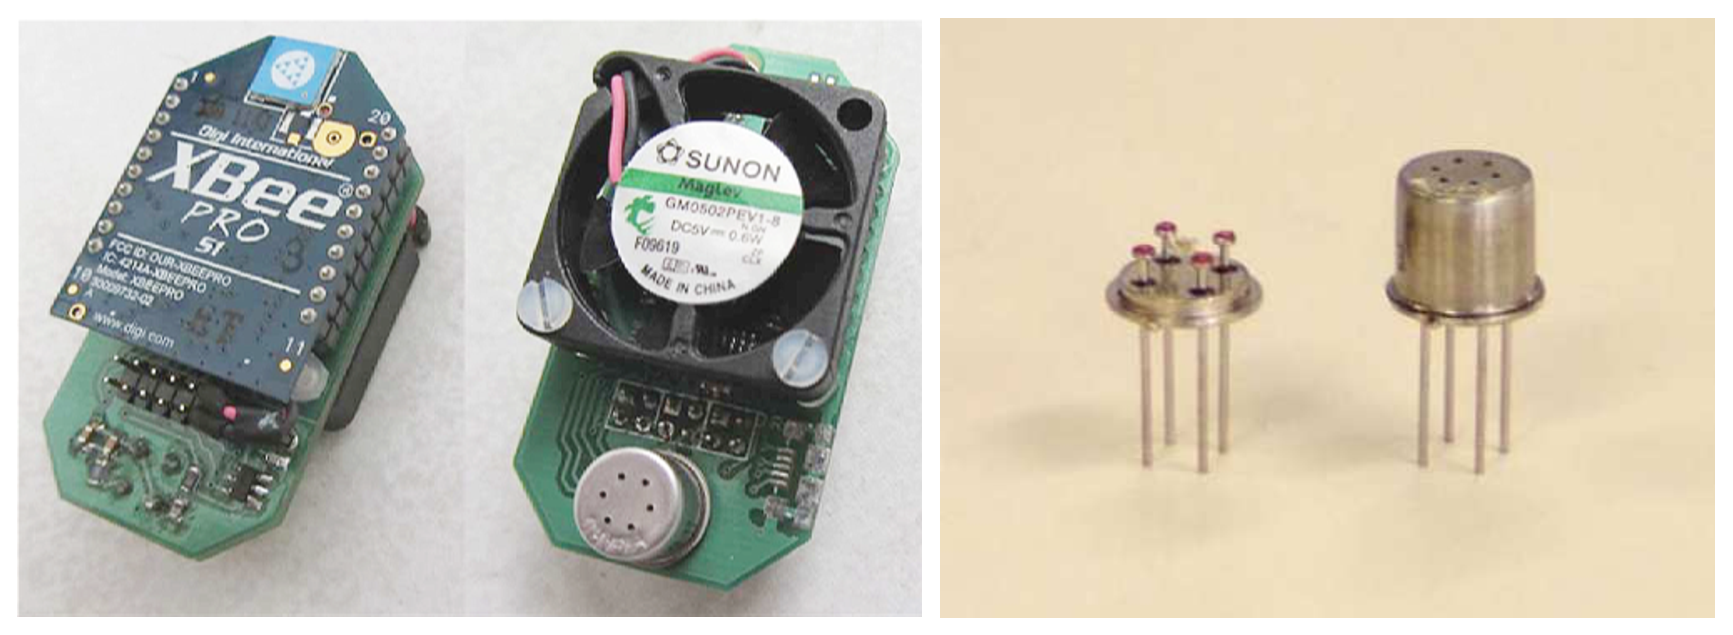
\includegraphics[width=15cm]{images/introduction/OlusAndTGS2600.eps}}}
\captionFigure{Olus2 artificial nose module and odor sensor detail}
{fig:introduction/OlusAndTGS2600}{
Olus2 modules (left) incorporate the TGS2600 odor sensor (right), which is based on tin dioxide semiconductor. Sources: \cite{vazquez2013integracion} and \url{http://figaro.com/}}
\end{figure}

%Odor source modeling
Whilst gas-sensor technology has becomed quite advanced in the last years \cite{pearce2003handbook}, there is still no ideal solution to be found, and the detection of odors has to rely on quite uncertain and noisy responses.
Even with a noisy sensory input, the odor search problem would be trivial to solve if odor concentrations were gradients that varied monotonically according to distance - but that is not the case. The random nature of odor plumes adds up into the equation and the complexity of the problem increases dramatically \cite{Torney2009}.
There is also variability in the types of odor sources that can be used as targets. As the molecular structure of scent particles provides each odorant with different fading times, it is not only needed to model the effective detection area of the odor plume but also its latency and evolution over time \cite{Mcgill2011}.


%Multimodal sensor integration
Having a good model of the target is then a crucial part towards the localization of odors, but those models must account for the uncertainty in the odor sensor response. These imprecisions, inherent to gas sensing, can be tackled with the particularly interesting approach that is multimodal sensor integration \cite{Hein24072012, song2011olfaction, arleo07}. The incorporation of other types of input from devices like video cameras, proximity sensors or air flow directivity sensors, can contribute to remove noise and increase the precision of odor plume detections \cite{Marjovi2013, Hayes02distributedodor}.
In the cases where the odor sources are not disperse but very localized instead, it can be possible to use a simple threshold model and obtain reasonable results \cite{vazquez2013integracion, acosta2013diseno}.




The other critical factor towards an efficient solution to the odor search task is the selection of a sensible search strategy. Search algorithms have been extensively studied for many decades, and the most popular approaches can be classified in three main groups: gradient-based algorithms (i.e. hill climbing \cite{Mcgill2011}), probabilistic methods (i.e. environment mapping \cite{FoxKo05}, bayesian, kalman or particle filters \cite{jatmiko2011robots}), and biologically inspired algorithms (i.e. biased random walks \cite{Hein24072012} or chaotic search \cite{KongcunM09}).
Gradient-based algorithms can be susceptible to local maxima and they depend on the monotonic variation of measurements, which as has been discussed is not the case for odor plumes. Probabilistic search methods and mapping, while requiring high computational resources and memory, are often the preferred approach when the environment is fully characterized.
Bio-inspired search algorithms, on the other hand, come into play when there is uncertainty within the definition of a search problem (i.e. when the search area is not well defined or odor sources may appear and disappear with different latencies).
All of these algorithms can be applied to single-agent tasks and to multi-robot search as well.


%\cite{Mcgill2011} % REVIEW General solutions to search of multiple emission sources
% The lack of a common set of validation cases and reference algorithms that form a ground truth for comparative analysis makes it impossible to directly compare the different algorithms and weigh their merits for different applications. This begs the questions of what should such a reference set involve and how should comparative analysis be performed. Some obvious characteristics are clearly relevant from the literature and evident in Table I: the initial distribution of sources and robots, the presence of obstacles, background flow, dead space (involving no perceptible gradient) and occluded sources, the level of disparity between source strengths, and the time-varying nature of source injection and removal.
% Gradient-based algorithms (i.e. hill climbing), which can be susceptible to local maxima.
% Probabilistic methods (i.e. mapping and bayesian, Kalman or particle filtering), which usually require high computational power
% Biologically inspired algorithms: biased random walks

%\cite{FoxKo05} % A Hierarchical Bayesian Approach to the Revisiting Problem in Mobile Robot Map Building





\subsection{Cooperative search strategies}

\vspace{-0.3cm}

Recent studies have shown that odor search algorithms that involve the collaboration among multiple robots can lead to a more efficient odor search \cite{Hu2013, Mcgill2011, marjovi2010olfactory}.
This project sets its focus on these approaches while leaving open the possibility of implementing single-robot strategies, as they can be considered the particular case of a \emph{N-robot} system where $N=1$.
Inter-robot cooperation can be implemented in various forms: an optimization of the available energy resources (i.e. live decision of which robot performs a surveillance task), by sharing mapping information \cite{Marjovi2011}, with the minimization of unnecessary redundancy during search, etc.
This kind of cooperativity among robots is covered by Appendix \ref{Appendix:designStrategies}.

Other types of collaboration can include multimodal sensory feedback as seen in some animal species. An interesting example of this approach is well reflected with an implementation where a robot would generate acoustic signals upon odor detection, and thus allow others reach the target much faster \cite{song2011olfaction}.
Supervised search where robots cooperate with humans to enhance the performance of a given search task \cite{GoodrichPendleton11, KonoligeOrtiz04}, can also be considered a form of multimodal sensory feedback.
Human-robot interaction already plays a crucial role in gas detection for environmental monitoring \cite{Dunbabin2012} as well as in search and rescue of targets \cite{Hu2013}.
Autonomous robot team management has also received inspiration from human behavior, for instance with the incorporation of dynamical team and sub-team creation \cite{BradshawFeltovich09} that leads to improvements in human-agent-robot interaction.

%\cite{Marjovi2011} % cooperative search in structured environments. robot communication (mapping)

%\cite{Hu2013} % cooperative search review, hybrid simulations

%\cite{song2011olfaction} % odor plume search real robots. multimodal sensors. one robot locates the odor and emmits a sound to attract other robots to the odor source

%----Human interaction in search

%\cite{Dunbabin2012} % Robots for Environmental Monitoring: Significant Advancements and Applications

%\cite{BradshawFeltovich09} % human-like team creation and management. joint activity coordination and cooperation with human entities. human-agent-robot teams. dinamical creation of teams and subteams

%\cite{GoodrichPendleton11} % human interaction with bio-inspired robot teams

%\cite{KonoligeOrtiz04} % Centibots: Very Large Scale Distributed Robotic Teams. human interaction. integrated end-to-end system


%----Emerging group-level intelligence through simple local interaction

Higher levels of cooperation can also be achieved without the need of a global deterministic specification of the search algorithms. Bio-inspired strategies that are based on \emph{swarm robotics} take advantage on the group-level intelligence that can emerge from simple local interactions, a subject with raising interest among the odor-locating research community \cite{Torney2009}.
Some experiments have already demonstrated the capability of a robot swarm to transverse an odor plume by the means of simple inter-robot interaction with soft-defined rules \cite{Marjovi2013}.
An example of these rules can be lightweight agent-avoidance routines that lead to a global exploratory behavior \cite{Marques2006}.
The behavioral rules can also be context-dependent. For instance, long-range exploration could be inhibited when local odors are detected or when energy resources are running low.

%\cite{Marjovi2013} % odor plume modeling and simulation, evaluation with real robots (roomba w/ laptops). swarm robotic formation (equally spaced, transversal line)

%\cite{Torney2009} % the task becomes highly nontrivial due to the generation of heterogeneous, dynamically changing filamental concentrations that do not decrease monotonically with distance to the source.
% odor search. emerging group-level intelligence. local interaction->emerging behavior

%\cite{Marques2006} % efficient local searching behaviours. By default, the agents tend to avoid each other, leading to the emergence of exploration behaviours when no chemical cue exists in the neighbourhood

\vspace{-0.5cm}
\subsubsection{Biased L\'{e}vy-walk search}
\vspace{-0.3cm}
%----Biased random search
While classical heuristic solutions could be adequate for the localization of odorants that have a fixed position and invariant properties, these are not an option for problems with uncertainty (i.e. a brute-force search algorithm would not be efficient for monitoring an area that is weakly defined).
On the other hand, bio-inspired strategies that do not rely on prior system assumptions could finally provide efficient solutions to the odor search task \cite{Hein24072012, Mcgill2011, raey10, arleo07}.
\emph{Random walks} or chaotic search have generally been the preferred source of inspiration for their robustness and performance within a reasonable simplicity \cite{KongcunM09}.
\emph{L\'{e}vy flights} are a specific type of random walk that can be commonly observed in nature \cite{Reynolds2013}.


\begin{figure}[h!]
\centerline{\mbox{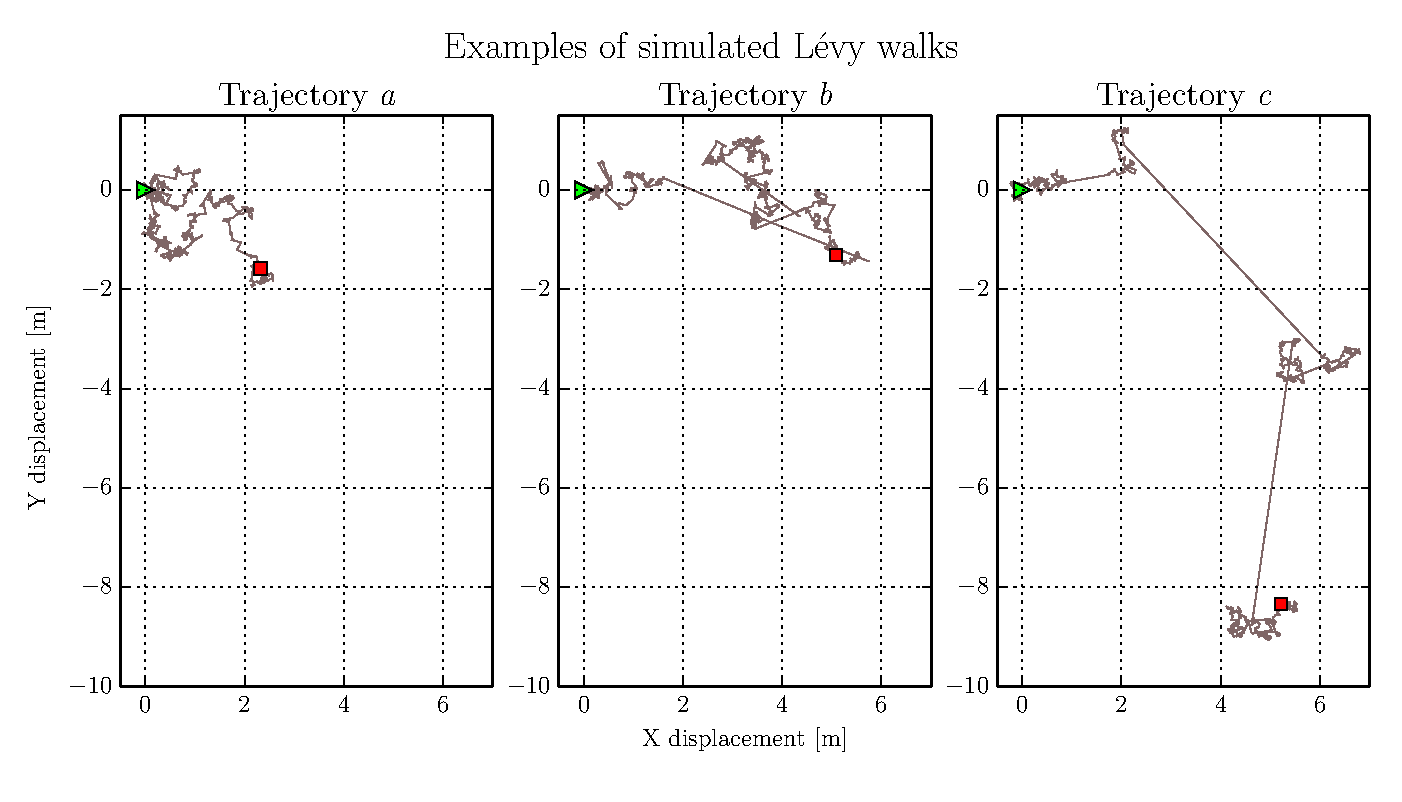
\includegraphics[width=15cm]{images/introduction/simulated_levy_walks.eps}}}
\captionFigure{Examples of simulated 2-dimensional L\'{e}vy walks}
{fig:introduction/simulated_levy_walks}{
2000 iterations of three different simulations that show various random walks based on a L\'{e}vy probabilistic distribution. The starting and ending points are marked in green and red respectively. Changes in the stability parameter $\alpha$ cause differences in the exploratory behavior: larger values generate a more localized search \emph{(a)}, while decreasing $\alpha$ can have the effect of a faster-growing expansion (\emph{b} and \emph{c}). The angular direction has a uniform distribution, but could also be nuanced in order to modulate the L\'{e}vy search strategy.
}
\end{figure}


They are formed by variable length steps that combine clusters of short-sized moves with more distant travel paths (see Fig. \ref{fig:introduction/simulated_levy_walks}). This variation in the length of the steps is determined by a L\'{e}vy probabilistic distribution that is heavy-tailed, which leads to a random occurrence of longer steps.
Species like honeybees, ants, marine predators, and even human hunters have shown the successful use of these L\'{e}vy patterns for search \cite{Raichlen23122013}.
As the behavior of animals and insects does not rely solely on random distributions, it can be possible to increase the eficiency by biasing the parameters of random navigation in real time with multimodal sensory input integration \cite{arleo07}. It has been shown that even the incorporation of feedback from a noisy sensor response can lead to a reduction in search times \cite{Hein24072012, KongcunM09}.

%\cite{arleo07} % multimodal sensory integration. navigation strategies. bio-inspiration

%\cite{raey10} % bio-inspiration for navigation strategies

%\cite{KongcunM09} % An Improved Artificial Fish Swarm Algorithm Based on Chaotic Search and Feedback Strategy. Clustering, optimization

%\cite{Hein24072012} % Sensing and decision-making in random search. multi-modal sensor integration. a lack of signal is not a lack of information. Searchers that receive no signal can quickly abandon target-poor regions. On the other hand, receiving a strong signal leads a searcher to concentrate search effort near targets. results show that including even a simple response to noisy sensory data can dominate other features of random search, resulting in lower mean search times


%----L\'{e}vy walks (Fig. \ref{fig:introduction/simulated_levy_walks})

%\cite{Reynolds2013} % levy walk model formulation % http://iopscience.iop.org/0295-5075/102/1/18001/article/
% Effective leadership in animal groups when no individual has pertinent information about resource locations: How interactions between leaders and followers can result in L\'{e}vy walk movement patterns

%\cite{Raichlen23122013} % evidence of levy walk in human hunters




The performance of many of these types of novel bio-inspired search strategies has yet to be evaluated for the odor search task. Whilst it is common to use simulators, it has already been discussed that the randomness of odorant plumes makes their modeling computationally inefficient. Hybrid simulators could be a solution for this issue, since they can combine the precision of actual odor source measurements with the performance obtained with off-line algorithm optimization \cite{HayesMG03}. Though, all these implementations would still need to step out of theoretical calculations towards the actual implementation and validation with robots in the real world.


%\cite{HayesMG01} % odor search. distributed algorithm. demonstrate group robots transverse odor plume. faithful simulator

%\cite{HayesMG03} % Off-line optimization and validation with real robots. einforcement learning algorithm to optimize performance across group size, showing that it can be useful not only for improving real world odor localization, but also for quantitatively characterizing the influence of group size on task performance


\vspace{-0.5cm}
\subsection{Existing robotic platforms}
%Open-source 3D-printable platforms

The need for real-world validation of odor search tasks raises the question of what are the available robotic platforms that can be used.
Among the requirements that can be specified are: the presence of odor sensors, a localization system to register the position of the robots over time, a well-dimensioned power source, and a reduced cost. Also, the ability to easily incorporate other multimodal sensor information is essential \cite{Hayes02distributedodor}, but is a feature commonly lacking in odor search implementations.
Another important requirement is the size of the robots, as they should be small in order to minimize unnecessary odor plume disturbances.
Most of the previous work that can be found on literature demonstrating implementations of odor search strategies have relied on platforms such as the \emph{iRobot}\footnote{\url{http://www.irobot.com/}} \cite{Marjovi2013, marjovi2010olfactory} or other proprietary solutions \cite{ElfwingDoya14, jatmiko2011robots, KonoligeOrtiz04, HayesMG03}. Those robots are lacking either a reduced size or a simple expandability, which can cause difficulties towards standardization of real-world odor search implementations.


\emph{Printbots} are open-source robotic platforms that can be 3D-printed \cite{GonzalezValero11miniskybot,ValeroGonzalez12creativity,Garcia-Saura2012,ValeroGonzalezOOML12}, and they could provide the low-cost expandability and repeatability that are needed for these multi-robot implementations. As they are open, Printbots can be evolved by the community and thus easily modified to incorporate the improvements made in any part of the world. This means, for instance, that a wind sensor integration made for a particular odor location study could be rapidly merged back into the original robot design, and thus make the replication and further evolution of the experiment conveniently accessible to other researchers.

%\cite{jatmiko2011robots} % Robots implementation for odor source localization using PSO algorithm. odor localization, real robots, 12 ceiling cameras

%\cite{KonoligeOrtiz04} % Centibots: Very Large Scale Distributed Robotic Teams. human interaction. integrated end-to-end system

%\cite{acosta2013diseno} % simula fuente de olor con una luz, usa placa beaglebone, open-loop motor control

%\cite{Hayes02distributedodor} % conducting polymer-based odor sensors possess the combination of speed and sensitivity necessary to enable real world odor plume tracing. simple local position, odor, and flow information, tightly coupled with robot behavior, is sufficient

%\cite{Marjovi2013} % odor plume modeling and simulation, evaluation with real robots (roomba w/ laptops). swarm robotic formation (equally spaced, transversal line)

%\cite{marjovi2010olfactory} % cooperative odor search, real robots, wireless network for robot localization










\vspace{-0.3cm}
\subsubsection{Spatial localization techniques}
\vspace{-0.3cm}
%Trabajo previo de tracking. GPS, Cámaras, etc

A good perception of the position of robot agents in their environment is necessary for some search algorithms. Most importantly, robot localization is needed at a experimental level in order to evaluate the performance of search strategies \cite{jatmiko2011robots, Fox00Pro}.
The field of automated robot tracking has been widely studied for many years, and a number of robust solutions have appeared \cite{Gut02Exp}. Whilst GPS (\emph{Global Positioning System}) is the preferred approach for outdoor environment, it only provides accuracy at the meter range and higher accuracies are needed for local or indoor search \cite{ChenSun10}.
The combination of GPS with other radio-frequency-based approaches (i.e. position inference based on GSM or Wi-Fi signal strength \cite{Ferris06gaussianprocesses}) can provide more resolution at the expense of a cost that does not scale for large robot swarms.
The cost of robot localization can be minimized with the use of more simple sensors, as it is possible to obtain accuracy from
devices that have noisy measurements
with the use of state-of-the-art technologies like artificial intelligence algorithms \cite{Thrun98landmark, FoxKo05}.

Landmark-based localization techniques (such as the use of beacons) are one of the most extended methods, as they can be applied to most types of input \cite{EscaleraMoreno96, Fox00Pro}. Most of the robot localization approaches for indoor environments are vision-based \cite{chen2009towards}. Some decide to place markers in the environment and mount cameras on board each robot \cite{gifford2009low, HongboHongnian07} while others place markers in the robots and then use external cameras to inform each robot of its position \cite{reina2012zeppelin, jatmiko2011robots}. This last alternative can be the most attractive for experimental research environments, since it provides a low cost solution and the added convenience of having the experiments recorded in video.




%\cite{Thrun98landmark} % Bayesian Landmark Learning for Mobile Robot Localization

%\cite{FoxKo05} % A Hierarchical Bayesian Approach to the Revisiting Problem in Mobile Robot Map Building


%\cite{EscaleraMoreno96} % Continuous mobile robot localization by using structured light and a geometric map



%\cite{Fox00Pro} % A Probabilistic Approach to Collaborative Multi-Robot Localization. cameras and laser rangefinders



%\cite{chen2009towards} % Towards multi-robot formations: study on vision-based localization system

%\cite{jatmiko2011robots} % Robots implementation for odor source localization using PSO algorithm. odor localization, real robots, 12 ceiling cameras

%\cite{reina2012zeppelin} % zePPeLIN: Ceiling camera networks for the distributed path planning of ground robots

%\cite{HongboHongnian07} % Ceiling Light Landmarks Based Localization and Motion Control for a Mobile Robot

%\cite{gifford2009low} % Low-Cost Mobile Robot Localization Using Only a Downward-Facing Webcam. OJO VA EN EL ROBOT



%\cite{Ferris06gaussianprocesses} % Gaussian Processes for Signal Strength-Based Location Estimation

%\cite{Gut02Exp} % An Experimental Comparison of Localization Methods Continued

%\cite{ChenSun10} % Localization for Multirobot Formations in Indoor Environment





\vspace{-0.5cm}
\lsection{Project approach, methodology and goals}

The high variability in the parameter definition of odor search problems (\emph{i.e. initial distribution of robots in the search area, presence of obstacles, amount of odor sources and their latency, etc.}) has caused the absence of a standardized method for directly validating nor comparing the performance of each search algorithm \cite{Mcgill2011}.
Part of the problem arises from the use of proprietary robotic platforms in previous studies, which are expensive and not suitable for more than a few algorithm implementations. The standardization around a robotic platform should then be of help towards a common base of comparison for odor search algorithms.

This project will try to address the issue, with the design of an open-source set of tools to allow the future implementation and field testing of a broad range of search algorithms with a set of low-cost replicateable robots.

The specific goals are:

\vspace{-0.5cm}

\begin{packed_enum}
	\item Design of a 3D printed structure for the mobile robots. It must be easy to replicate the robot to create a swarm of low-cost identical agents.
	\item Layout of the electronic boards, it is a requisite that they are energy efficient, have multi-sensor integration (an active artificial nose, battery monitoring, and also temperature, humidity and distance sensors), and based on Arduino.
	\item Selection of the technique for localizing the robots in the search space.
	\item Design and implementation of the bi-directional communication method that allows simple access to the experiment data in real time, with an abstraction layer in Python to allow high-level programming of the robots.
	\item Implementation of a closed-loop robot controller based on way points.
	\item Validation of the robot platform for odor detection.
	\item Assembly of at least three robots equipped with artificial noses.
	\item Open-source publication of the platform.
\end{packed_enum}

\vspace{0.0001cm}







\subsection{Relation with the Degree in ITST}
Being a multidisciplinar project, the required technical knowledge has been covered by most of the courses of the Degree in Telecommunication Technology and Service Engineering (ITST) at Universidad Aut\'{o}noma de Madrid.
Some specific courses from the itinerary on \emph{Design and Implementation of Electronic Communication Systems} have resulted of special interest (\emph{Sistemas de Control}, \emph{Sistemas Electr\'{o}nicos Digitales}, \emph{Instrumentaci\'{o}n y Medida}, \emph{Tecnolog\'{i}a Electr\'{o}nica de Sistemas}), and the core subjects have also received complementary education in the fields of electronics (\emph{Tecnolog\'{i}a de dispositivos}, \emph{Circuitos electr\'{o}nicos digitales}, \emph{Circuitos anal\'{o}gicos y de potencia}, \emph{Fundamentos de microprocesadores}), software and signal processing (\emph{Programaci\'{o}n I y II}, \emph{Sistemas lineales}, \emph{Teor\'{i}a de la comunicaci\'{o}n}, \emph{Tratamiento digital de se\~{n}ales}, \emph{Aritm\'{e}tica para el procesamiento de se\~{n}al}), as well as real-time networking (\emph{Redes I y II}, \emph{Redes Multimedia}).





\singlespacing
\subsection{Overview and milestones of the project}
\begin{enumerate}
	\item \textbf{Documentation and literature research (state of the art)}
	\item \textbf{\emph{GNBot} robotic platform design}
	\begin{enumerate}
		\item Printed mechanical structure
		\begin{enumerate}
			\item Design of the 3D parts (chassis, wheels, electronic board and battery supports, etc.)
			\item Motor type selection (two continuous rotation servomotors)
			\item Power requirement analysis and battery selection (two 9V rechargeable batteries)
		\end{enumerate}
		\item Electronic elements
		\begin{enumerate}
			\item Design of a PCB for the multi-sensor integration (including polarization circuits for the odor sensor, battery level monitor, luminosity sensors, IR range finders, an electronic compass, and the temperature and humidity sensor)
			\item Industrial manufacture of the designed circuit boards (20 unit order to \url{http://www.seeedstudio.com/})
		\end{enumerate}
		\item Software and communication interface
		\begin{enumerate}
			\item Development of the low-level control routines for Arduino
			\item Development of the ZigBee-based wireless communication protocol
			\item Development of the abstraction layer with Python
		\end{enumerate}
	\end{enumerate}
	\item \textbf{Assembly, testing and experiments}
	\begin{enumerate}
		\item Assembly and test of the prototype GNBot
		\item Implementation of a light landmark based localization system (documented in Appendix \ref{Appendix:lightLandmarks}).
		\item Design of the vision-based automatic robot tracking software (OpenCV and Python), adapted to the developed visual markers to provide X-Y position and angle orientation feedback
		\item Battery duration and performance measurements
		\item Implementation of a closed-loop way-point navigation algorithm
		\item Fabrication of the low-profile odor sources, to be used as targets for the search
		\item Robot platform multimodal sensor range characterization
		\item Assembly and test of a swarm of four final-version GNBot robots
	\end{enumerate}
	\item \textbf{Publication, contest participation and documentation}
	\begin{enumerate}
		\item \textbf{Publication submission and acceptance to the \emph{Living Machines 2014} International conference}, and participation of the project in the \emph{Arquimedes National Research Contest}. See Appendix \ref{Appendix:circuits}
		\item Creation of a website and GitHub repository for the open-source publication of the developed GNBot platform
	\end{enumerate}
\end{enumerate}
\onehalfspacing

The lenght of the project has been 12 months, at a rate of 3 hours/day. With the open-source publication of the developed platform the author expects to have contributed towards an acceleration in the development of cooperative robotic odor localization strategies.

Website of the GNBot project:  \url{https://github.com/carlosgs/GNBot/}


\newpage \thispagestyle{empty} % Página vacía



%\input{cap_intro_bio}

%\input{cap_sistemas}

%\input{chapters/chap2_stateoftheart}

\chapter{Design and development of the GNBot odor-sensing robotic platform}
\label{chap:design}
\vspace{-1cm}


For the robot design, existing open-source projects were used as a base. The preferred designs had most mechanical parts intended to be manufactured with a low-cost 3D printer. These are called \emph{printbots} \cite{GonzalezValero11miniskybot, ValeroGonzalez12creativity, ValeroGonzalezOOML12}, and one example is the MiniSkybot\footnote{\url{http://www.iearobotics.com/wiki/index.php?title=Miniskybot\_2}}. Printbots provide an accelerated design path not only for creating basic educational tools \cite{Garcia-Saura2012} but also for making robots that can be used for research, such as the platform presented in this work.
With this technique it is possible to easily reuse, develop and incorporate the most useful parts of previous designs in order to fulfill the requirements of a robot needed for a given task.

Regarding swarm robotics, printbots have been preferred over other solutions for both the reduced manufacture cost and, most importantly, for the high adaptability of the designs to the search problems. For instance, the use of 3D printed structures opens the possibility of easily testing the performance of various spatial distributions of the odor sensors in the robot, by manufacturing custom parts that can accommodate the different configurations.




The proposed robot design (shown in Fig. \ref{fig:design/GNBot_iterations}) is a derivative of the ArduSkybot\footnote{\url{https://github.com/carlosgs/ArduSkybot}}, an educational printbot based on the Arduino\footnote{\url{http://arduino.cc}} UNO electronic board, and it also incorporates work from the Vector-9000\footnote{\url{https://github.com/carlosgs/carlosgs-designs/tree/master/Vector-9000-a-fast-line-follower-robot}} competition robot. 
From these projects, integration was made in respect to hardware (mechanical parts and electronic boards) and software (robot firmware and a basic communication strategy) aspects.
On the hardware side, the ArduSkybot design was modified to incorporate the Arduino MEGA board to allow the addition of more sensors.

%\vspace{1cm}

\begin{figure}[h!]
\centerline{\mbox{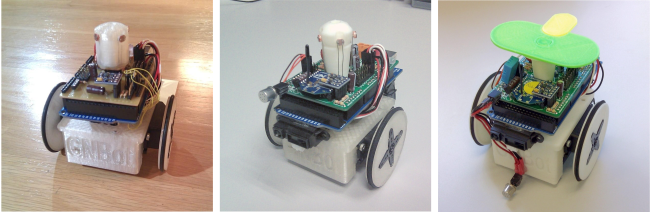
\includegraphics[width=16cm]{images/design/GNBot_iterations.eps}}}
\captionFigure{The three GNBot versions that were developed}
{fig:design/GNBot_iterations}{
From left to right: GNBot version alpha, v0.1 and v1.0 (the current version).
The two earlier designs had a light sensor array placed on the top (intended for light landmark identification as shown in Appendix \ref{Appendix:lightLandmarks}), while the latest version has a two-color marker (intended for the automated visual position tracking in Section \ref{sect:visionBasedLocalization}). %Both subjects are explained in further sections.
}\end{figure}

\vspace{-1cm}



\lsection{Open-source electronics}
\label{sect:openSourceElectronics}


The Printshield board -designed for the ArduSkybot- was the base to design the GNBoard (see Fig. \ref{fig:design/GNBoard_prototypeAndFinal}), which provides a compact solution that contains most sensors and allows an easier interconnection. The GNBot also incorporated a light sensor array developed originally for the Vector-9000, and that project also provided the software base with a framework to interface with the computer in a fault-tolerant manner. All of the PCB designs (schematics and circuit layout) were designed using the \emph{KiCad EDA Software Suite}\footnote{\url{http://www.kicad-pcb.org/}}, an open-source tool.




\begin{figure}[h!]
\centerline{\mbox{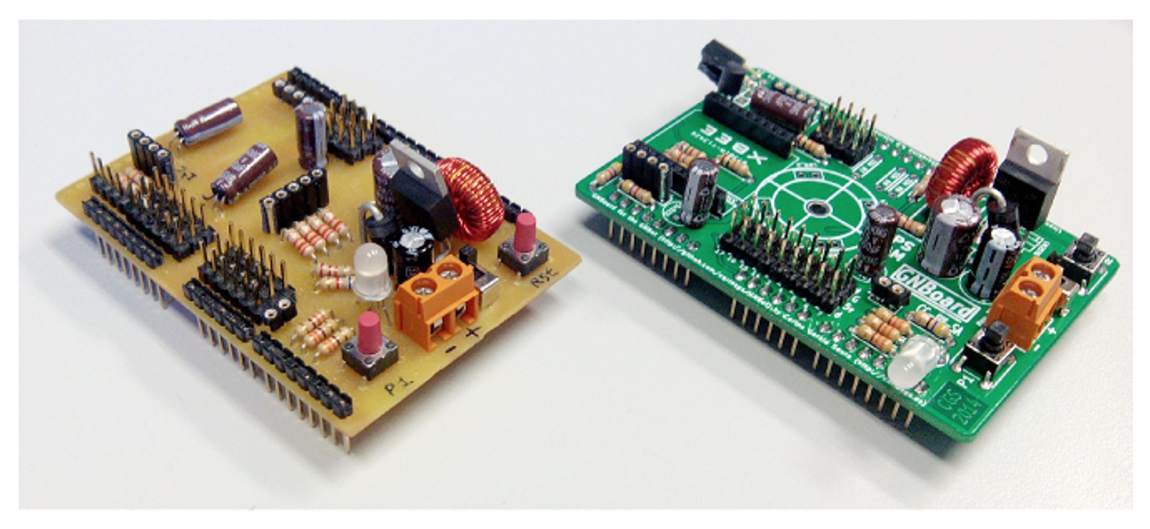
\includegraphics[width=15cm]{images/design/GNBoard_prototypeAndFinal.eps}}}
\captionFigure{The two versions of the GNBoard developed for this project}
{fig:design/GNBoard_prototypeAndFinal}{
Prototype design (left) and version 1.0 (right).
The boards are designed to plug into an \emph{Arduino MEGA}.
Schematics and layout can be found in Appendix \ref{Appendix:circuits}.
}\end{figure}






The motion of the robot is achieved using two continuous rotation servomotors (\emph{SM-S4303R}) as the main actuators. Servomotors provide a compact and low-cost solution to achieve the digital speed control needed, and they are frequently used in bio-inspired robot designs \cite{zamorano2011control,Herrero11,Urziceanu11,MeyerSproewitz06}.
%\cite{zamorano2011control} % Control locomotor multidireccional de un robot modular mediante circuitos generadores centrales de patrones bioinspirados
%\cite{Herrero11} % Bio-inspired design strategies for central pattern generator control in modular robotics
%\cite{Urziceanu11} % Central pattern generator control of a differential wheeled robot
%\cite{MeyerSproewitz06} % Passive compliance for an ({RC}) servo-controlled bouncing robot
The main downside of this kind of actuator is the high current demand -particularly during transient motions- which requires the use of an adequate power supply. For the GNBoard the design decision was to use a switching power supply (shown in Fig. \ref{fig:design/GNBoard_PSU}) rather than a linear regulator, provided the much higher efficiency.
\begin{figure}[h!]
\centerline{\mbox{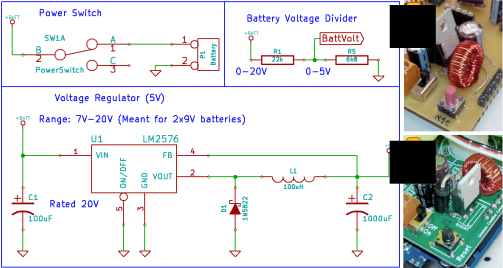
\includegraphics[width=12cm]{images/design/GNBoard_PSU.eps}}}
\captionFigure{Power supply schematic and actual assembly}
{fig:design/GNBoard_PSU}{
\emph{A)} and \emph{B)} respectively show the power supplies in GNBoard v0.1 and v1.0 (final version).
The power supply of the GNBoard uses an \emph{LM2576-5} switching regulator that is capable of delivering up to 3A, which is more than sufficient to cover the energy demand of the entire robot.
}\end{figure}
Switching power regulators also have a broad input voltage range, allowing to make better use of the full capacity of the batteries since they can be connected in series without negative effect in the performance.

The other incorporated element was a battery voltage monitor, which has been designed to be used for resource-wise decision making in search strategies. The implementation of this sensing capability was done by placing a resistive voltage divider (also shown in Fig. \ref{fig:design/GNBoard_PSU}) that adapts battery voltage to the $[0,5]V$ range that can be measured with the Arduino board.


The selection of sensory input was oriented towards the odor source localization task, and thus an electronic nose was made part of the robot (see Fig. \ref{fig:design/artificialNose_polarization}).

\begin{figure}[h!]
\centerline{\mbox{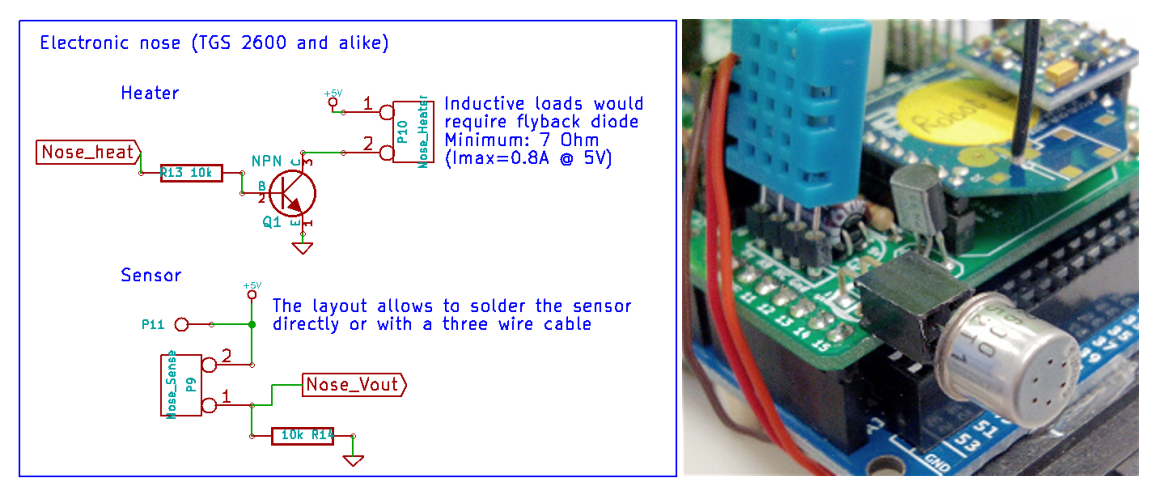
\includegraphics[width=14cm]{images/design/artificialNose_polarization.eps}}}
\captionFigure{Polarization scheme for the artificial nose sensor and detail picture of the assembly}
{fig:design/artificialNose_polarization}{
The mounted sensor is the \emph{TGS-2600} gas detector from \url{http://www.figarosensor.com/}, but any kind of sensor with a similar polarization scheme (as shown in the left panel) could be used.
}\end{figure}

The odor sensor works with a heater element whose temperature can be controlled electronically by a power transistor placed for this purpose on the GNBoard.
Odor sensor temperature control allows the usage of different modulation strategies to enhance sensor performance and to allow adaptation to the intensity of odor sources \cite{YanezToledano12}. 
Robots also incorporate an infra-red analog rangefinder (ref: \emph{Sharp GP2Y0A21}) to avoid collision with obstacles and other robots within the search environment, as well as a light sensor array intended to be used to identify light landmarks.
A temperature and humidity sensor (ref: \emph{Aosong DHT11}) is also present in the GNBoard.
Finally, an electronic compass (ref: \emph{Honeywell HMC5883L}) provides the orientation knowledge.
This way, each robot and the swarm can have a basic multimodal perception of their status and location in the search area.

Overall the GNBoard designed for this project allows the incorporation of multiple sensors and facilitates software-hardware integration, as it is an essential requirement for the efficient implementation of odor search tasks that have uncertainty. Next section will cover the selection of the communication system.


\vspace{-0.5cm}

\lsection{Communication with the robots}

In the case of collaborative swarm robots, one of the key design decisions that needs to be made is the selection of a proper communication method. Not only there is a trade-off between the \emph{working range, maximum information throughput and cost}, but there are some other facts that must also be taken into account:
\begin{packed_itemize}
\item \emph{Working environment:} Radio-Frequency (RF) communications generally provide a robust system for most applications, but sometimes other solutions can provide a better balance between performance and cost. For instance, for underwater applications RF signal attenuation may become an issue, and the use of sound waves, light pulses, or even tethering with a cable become reasonable options.
\item \emph{Power requirements, adaptivity and remote-end sensing:} Since mobile robots have very limited energy resources, an efficient system should be generally preferred in order to maximize the operation time. In the same line, some interfaces provide a way to switch among different power schemes in real time, as well as having the capability to measure the signal intensity received from the other end. These should be preferred since the adaptivity in communications is key towards an optimal usage of energy resources.
\item \emph{Networking capability:} Not all communication systems offer the possibility to address data to different end nodes, and this is a must to allow scaling up the size of the swarm. This factor is crucial towards the efficient implementation of inter-robot communication.
\end{packed_itemize}

ZigBee\footnote{\url{http://www.digi.com/technology/rf-articles/wireless-zigbee}} (\emph{IEEE 802.15.4}) has been chosen from all of the available integrated solutions, since it is a highly configurable platform that is compatible with most of the points detailed above (see Table \ref{tab:design/xbee_wifi_bt_comparison} for a technical comparison). It provides an excellent networking layer, and since it is designed for low power applications, ZigBee has the possibility of adapting RF energy usage in real time.


\begin{table}[h!]
\centerline{\mbox{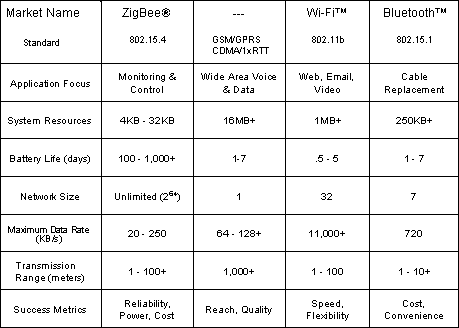
\includegraphics[width=12.5cm]{images/design/xbee_wifi_bt_comparison.png}}}
\captionTable{Comparison of the ZigBee, GPRS/GSM, Wi-Fi and Bluetooth wireless communication protocols}
{tab:design/xbee_wifi_bt_comparison}{
Source: ZigBee Alliance
}\end{table}


The main downsides of the ZigBee solution are the maximum throughput rates and the timing constrains, which must be taken into account when considering the use of more complex sensory input such as real time video streams.

Incorporation of the ZigBee modules into the GNBoard needed some special considerations (see Fig. \ref{fig:design/GNBoard_ZigBee}), as the selected modules work on 3.3V signals while the Arduino and GNBoard run on 5V.

\begin{figure}[h!]
\centerline{\mbox{\includegraphics[width=14cm]{images/design/GNBoard_ZigBee.eps}}}
\captionFigure{ZigBee connection schematic and its actual place in the GNBoard}
{fig:design/GNBoard_ZigBee}{
The selected ZigBee-compatible module is the \emph{XBee S2 (XB24-BWIT-004)}.
A 3.3V power line was reutilized from the regulator already present in the Arduino MEGA board. Adaptation of the TTL signal levels for the $Arduino \rightarrow ZigBee$ path was done using a resistive voltage divider. The $ZigBee \rightarrow Arduino$ path, on the other hand, did not require adaptation of the voltage level, since 3.3V TTL is correctly interpreted by the Atmel processor present in the Arduino board.
A decoupling capacitor was added to the 3.3V power line, and both of the transmission lines are terminated with resistors in order to maximize signal integrity.
}\end{figure}




Communication with the robots through these modules is asynchronous with a best-effort policy for packet forwarding, and thus real time event handling is critical. Data links must be fault tolerant, which can be achieved by using redundancy to ensure that messages are received and processed correctly by each node, and soft-state should be preferred to avoid deadlocks and allow fast recovery.
Reliability in communications is a key element to implement the virtualized network topology explained in next section.


\subsection{The ZigBee-based abstraction layer}

Odor search algorithms may rely on very different network topologies to maximize the chances of successful search and minimize time or energy consumption while, at the same time, dealing with context-specific communication range restrictions. In particular, the spatial scale of the search problem and the actual detection range of the odor sources are important factors to design the network topology, which could be changed for instance according to the energy level information.
As shown in Figure \ref{fig:design/topology}, a base tree topology makes it possible to emulate and test many different architectures.



\begin{figure}[h!]
\centerline{\mbox{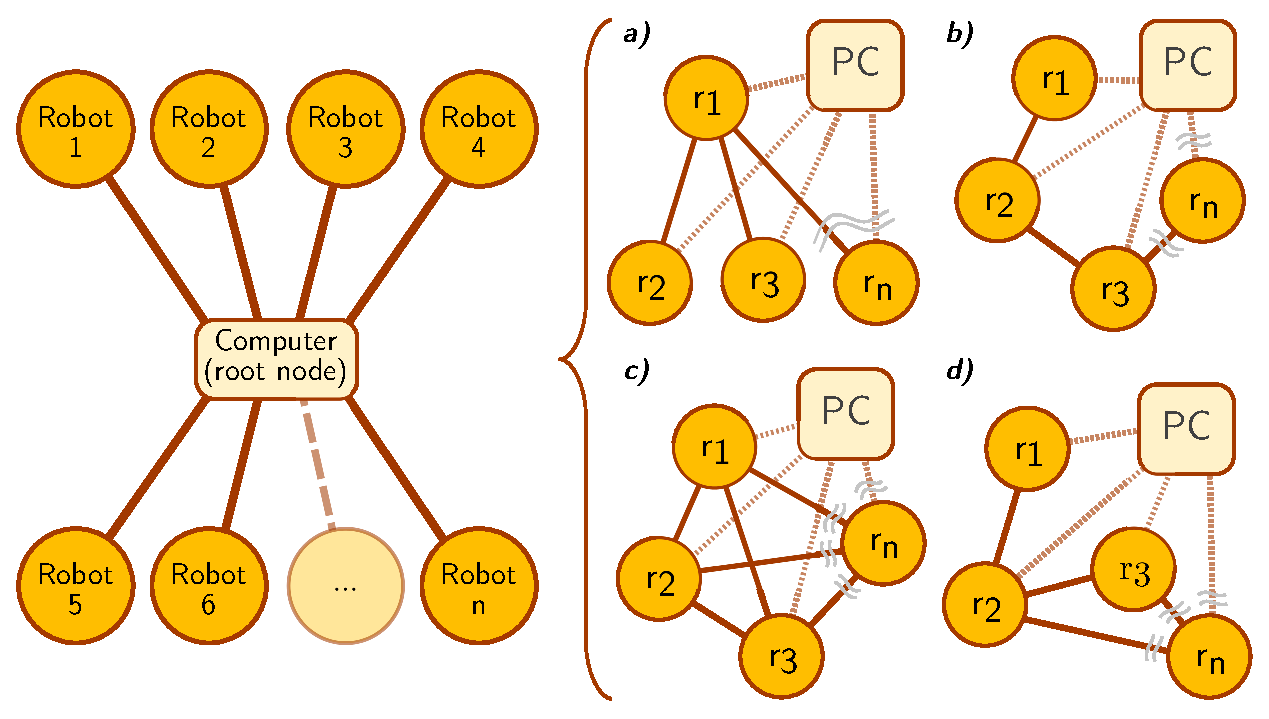
\includegraphics[width=15cm]{images/design/topology.eps}}}
\captionFigure{Possible virtualizations of the network topology}
{fig:design/topology}{
The star architecture shown on the left serves as the base to emulate a wide range of topologies. While underlying communications are centralized, the implemented algorithms can have very different requirements. As all information flows through the central computer, virtualized connectivities between robots can be defined in order to achieve various architectures such as \emph{a) tree/star}, \emph{b) line}, \emph{c) fully interconnected}, or \emph{d) mesh}, among others. The emulation of many other characteristics of physical links (\emph{variable delays, jitter, data corruption, packet loss...}) could be used to test the resilience of the implemented search algorithms in a controlled manner.
}\end{figure}


The approach used is to abstract all the calculations to a root computer, effectively using each robot as a peripheral.
A centralized infrastructure is used to command each autonomous robot independently, but a convenient layer of abstraction will also allow testing algorithms that are decentralized (see panels \emph{a-d} in Fig. \ref{fig:design/topology}). Main advantages of this approach are:
%\begin{packed_itemize}
\begin{itemize}
\item First, it is able to reduce costs since robots are kept simple, with reduced computational ability. For a fixed funding, cutting down the cost of each robot makes it possible to create more of them and thus have a bigger swarm.
\item Second, as all data flows through the root node, it can be logged and analyzed in order to evaluate the performance of each algorithm and allows easier debugging. Having all information in one place is particularly convenient when testing distributed algorithms.
\item Third, it provides a layer of abstraction. The code that specifies the behavior of each robot runs on the central computer, and thus a high-level programming language can be used (Python\footnote{\url{http://www.python.org/}} was selected for this project). This way it is possible to focus on developing the algorithms rather than dealing with the limitations of memory and power of the micro-controller on board each robot.
\item Finally, it is important to emphasize that the centralized architecture supports a large dynamic range of complexity of the algorithms, that can be kept simple (i.e. chaotic search~\cite{KongcunM09}) or complex (i.e. particle filtering~\cite{Marques2006}).
\end{itemize}
%\end{packed_itemize}

The emulated topologies could be dynamically reconfigured in real time to adapt to the search requirements (i.e. groups of robots may establish separate sub-networks when getting far from others to do local search, and later share the search results with the rest of the group).
The chosen ZigBee communication protocol natively supports the deployment of such architectures in the real world, which makes it very convenient towards the actual implementation of the virtually-optimized topologies.











\lsection{Real time robot position measurement}
\label{sect:realTimePositionMeasurement}

Knowledge of the position that each robot has in the area of the experiment is not only needed as input for some search strategies, but also for the evaluation of the performance of search algorithms in general. The trajectories undertaken by each robot can be useful information that allows the measurement of redundancy, interaction and efficiency during the performance of an odor localization task.

For this project, a new multimodal approach for robot localization was developed and evaluated. The idea was to use purposely-placed light sources as landmarks that allow each robot the identification of their relative positions within the search area. Unfortunately, the electronic compass sensor that provided the orientation measurements needed did not perform as expected (due to magnetic field distortion indoors) and the method had to be discarded for its noisy position results. All the information regarding this technique can be found in Appendix \ref{Appendix:lightLandmarks}.


\subsection{Vision-based robot localization}
\label{sect:visionBasedLocalization}

Among the other robot localization approaches studied, the most convenient method was the use of computer vision algorithms in combination with visual markers on board each robot.
This technique required the use of an external camera observing the space where robots move, as well as color markers placed in the robots.
The developed visual markers (in Fig. \ref{fig:design/GNBot_opencv_markers}) were designed to be 3D-printed, as are the rest of the GNBot parts.
These markers have two distinguished colors in order to achieve the measurement of both XY position and rotation of the robots.
Rotation feedback is also necessary since the electronic compass measurements had proved to be quite noisy for indoor spaces (see Appendix \ref{Appendix:lightLandmarks}).





%\subsubsection{Design of the visual position markers}

\begin{figure}[h!]
\centerline{\mbox{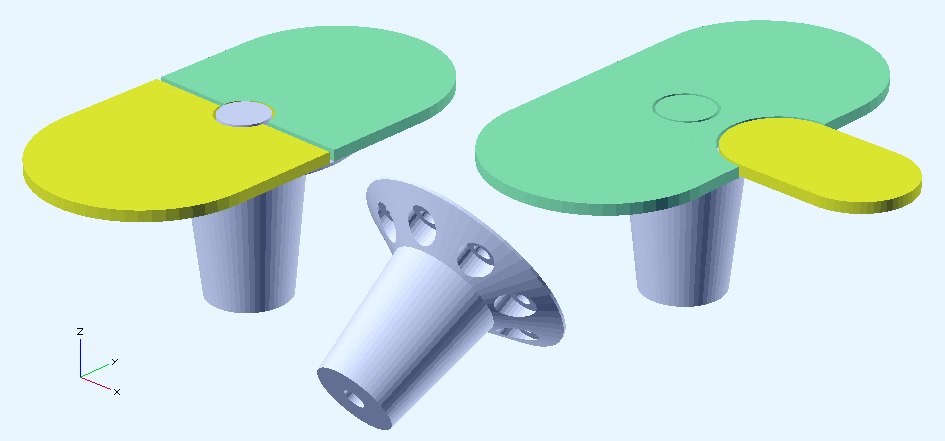
\includegraphics[width=12cm]{images/design/GNBot_opencv_markers.png}}}
\captionFigure{GNBot general purpose attachment piece and 3D-printed visual markers}
{fig:design/GNBot_opencv_markers}{
First and final versions of the markers used for computer-vision robot localization are shown in the left and right respectively. The part in the center is the attachment piece that allows to mount these markers and any other custom parts into the GNBot.
}\end{figure}







For measuring 2D positions, at first glance the best place for the external camera would be the ceiling right over the monitored area, in order to minimize distortion.
That way it would be possible to linearly map the observed robot position in the camera video with its actual location in the real world.
But as manually obtaining an adequate camera alignment is laborious and error-prone, another solution can be to calibrate the camera position using image processing software. Perspective correction
(see Fig. \ref{fig:design/perspective_correction})
simplifies this process: the user only needs to specify the position within the captured video of four reference points whose real location and dimensions are known.
\begin{figure}[h!]
\centerline{\mbox{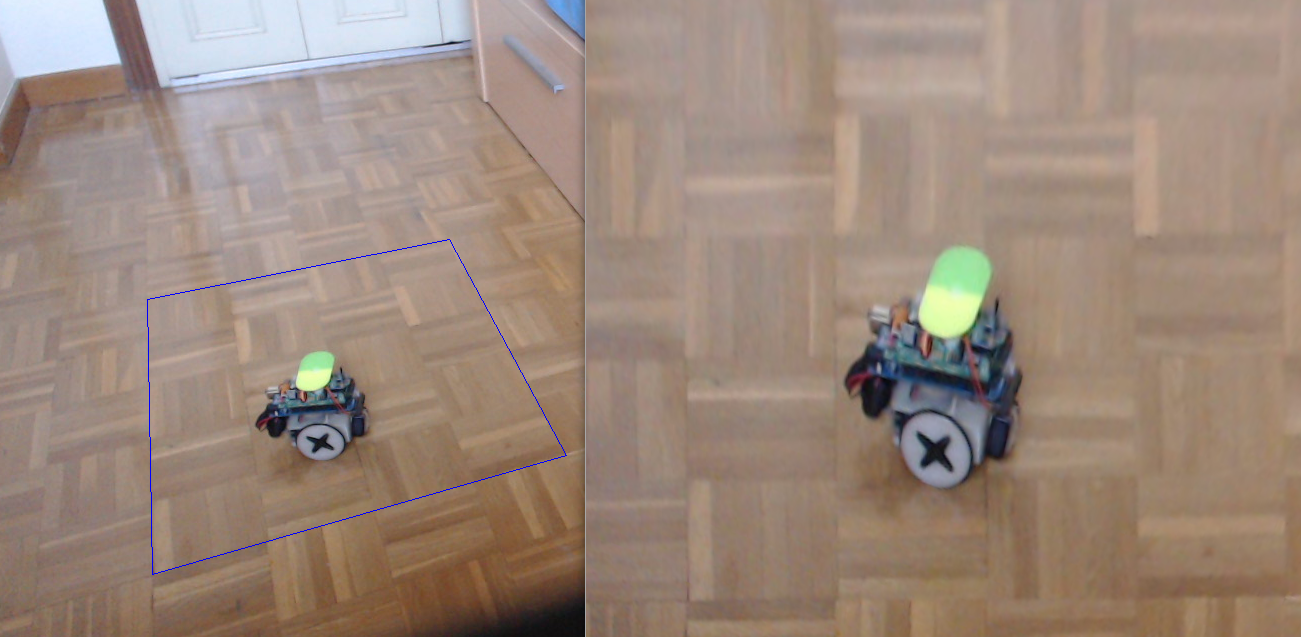
\includegraphics[width=11cm]{images/design/perspective_correction.png}}}
\captionFigure{Example of the video perspective correction}
{fig:design/perspective_correction}{
The original video stream is shown on the left, and the result of the perspective correction is shown on the right. The perspective has to be corrected in order to account for the visual distortion of the observed targets. This way, the X-Y position of each robot becomes linearly-proportional to the pixel positions in the video stream and can be directly mapped.
}
\end{figure}
The perspective correction technique is commonly used in many fields such as the aerospace industry for satellite surveillance or animal tracking for neuroethological research.

OpenCV\footnote{\url{http://www.opencv.org/}} was used for implementing the marker tracking software, as it is a convenient library that provides an efficient bundle of all the necessary image processing functions.
The full tracking process is explained in Figures \ref{fig:design/opencv_tracking_steps} and \ref{fig:design/opencv_tracking_steps_angle}.



\begin{figure}[h!]
\centerline{\mbox{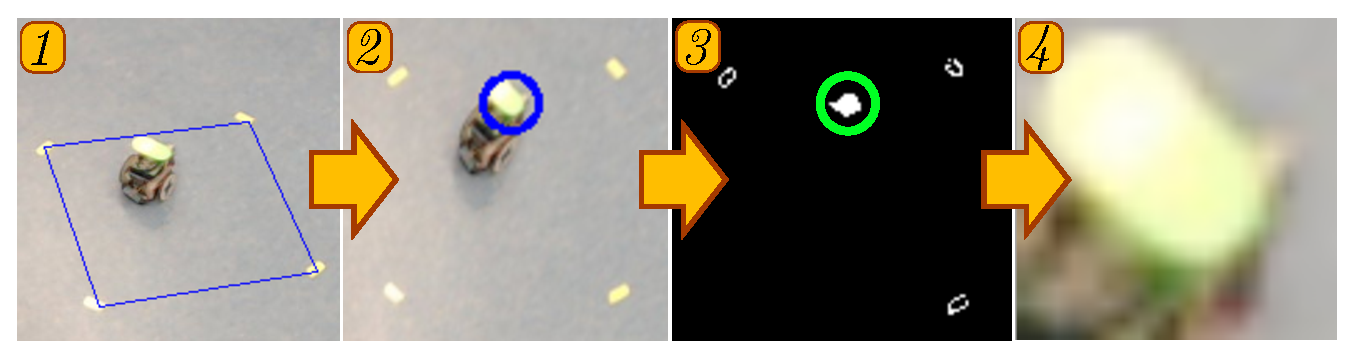
\includegraphics[width=15cm]{images/design/opencv_tracking_steps.eps}}}
\captionFigure{Steps of the marker position detection algorithm}
{fig:design/opencv_tracking_steps}{
In a first step, the user manually specifies the reference points in the original video stream \emph{(1)} by using the mouse. The rest of the process is automated, with the creation of a corrected perspective image \emph{(2)}, the application of a threshold that focuses on the marker color \emph{(3)}, and the detection of the largest spot, which will finally output the coordinates of the robot. Afterwards, the \emph{region of interest} is segmented \emph{(4)} for the next step of the algorithm: robot orientation measurement (see Fig. \ref{fig:design/opencv_tracking_steps_angle}).
}\end{figure}




\begin{figure}[h!]
\centerline{\mbox{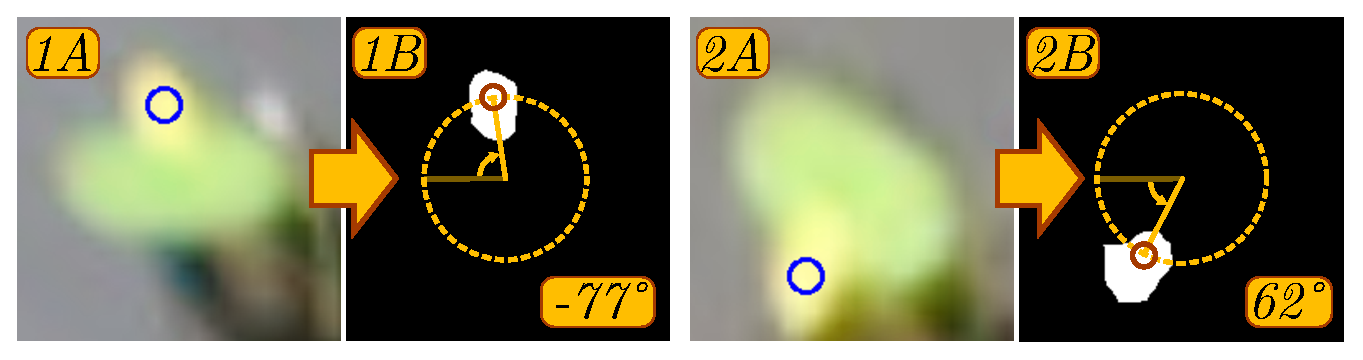
\includegraphics[width=15cm]{images/design/opencv_tracking_steps_angle.eps}}}
\captionFigure{Marker orientation detection algorithm}
{fig:design/opencv_tracking_steps_angle}{
\emph{1A} and \emph{2A} show the segmented ``region of interest'' from the previous part of the tracking algorithm (see Fig. \ref{fig:design/opencv_tracking_steps}), displaying the corrected-perspective marker in the middle. As the largest color of the marker (green) is centered, it is then possible to apply a threshold \emph{(2A},\emph{2B)} that focuses on the sub-marker (yellow) to obtain its position. Finally, the robot rotation angle is calculated according to the relative position of the sub-marker with respect to the center.
}\end{figure}


The software was fully implemented in Python for this project, using only standardized OpenCV functions (\texttt{cv2.getPerspectiveTransform}, \texttt{cv2.warpPerspective}, \texttt{cv2.cvtColor}, \texttt{cv2.inRange}, and \texttt{cv2.findContours}).
Also, the developed system is open-source and can be easily re-purposed for other video tracking tasks.



\vspace{-0.5cm}
\lsection{3D-printable hardware design}
\vspace{-0.2cm}
From the specification of the project, the GNBot design was oriented towards cost reduction and easy replication.
Fig. \ref{fig:design/GNBot_parts} shows all the components that are needed to assemble one robot, and the resulting GNBot is shown in Fig. \ref{fig:design/GNBot_views}.

\begin{figure}[h!]
\centerline{\mbox{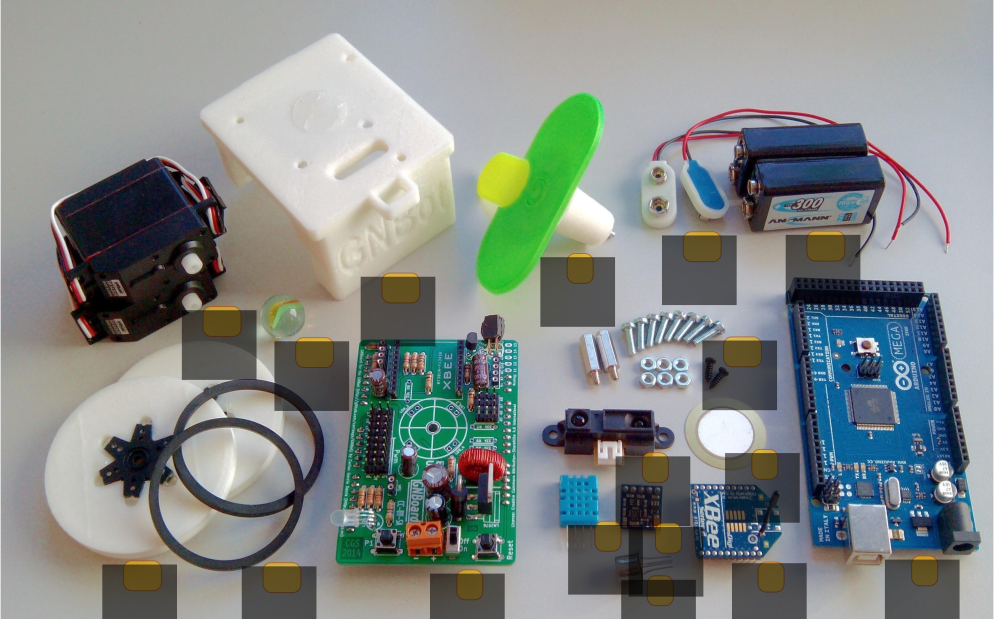
\includegraphics[width=16cm]{images/design/GNBot_parts.eps}}}
\captionFigure{Detail of the parts that form one GNBot v1.0}
{fig:design/GNBot_parts}{
Items shown in the picture:
\emph{1)} GNBoard electronics.
\emph{2)} Arduino MEGA board.
\emph{3)} TGS-2600 odor sensor.
\emph{4)} ZigBee-compatible RF module.
\emph{5)} Infra-red distance sensor.
\emph{6)} DHT11 temperature and humidity sensor.
\emph{7)} HMC5883L magnetometer sensor.
\emph{8)} Piezoelectric buzzer.
\emph{9)} Visual marker attachment.
\emph{10)} Two 9V battery connectors.
\emph{11)} Two 9V rechargeable batteries (300mAh).
\emph{12)} Two continuous-rotation servomotors.
\emph{13)} 3D-printed robot wheels.
\emph{14)} Rubber outer-wheel rings.
\emph{15)} 3D-printed GNBot chassis.
\emph{16)} Marble for the idler wheel.
}\end{figure}

%\vspace{-0.2cm}
The only custom items that are present in the design are the GNBoard electronics and the 3D-printed parts (robot chassis, wheels and battery holder), which can be manufactured at a low cost. All of the other components are standardized and widely available.
The assembly of each robot is a simple process that only requires the use of standard tools (a flathead screwdriver, cutting pliers, and a hot-melt glue gun).

\begin{figure}[h!]
\centerline{\mbox{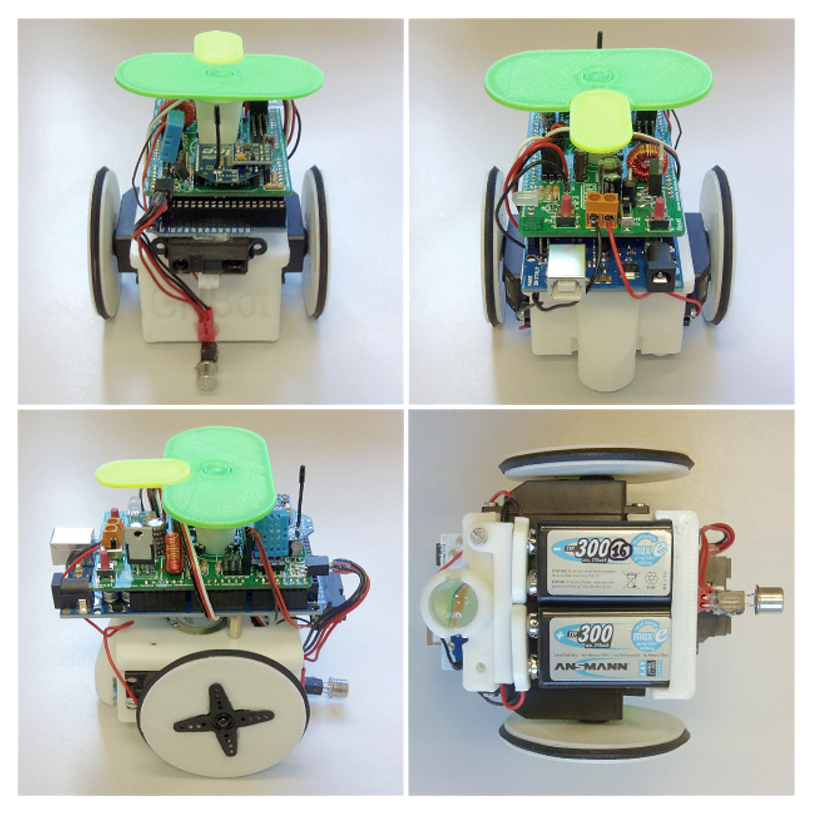
\includegraphics[width=13.5cm]{images/design/GNBot_views.eps}}}
\captionFigure{Assembled GNBot v1.0}
{fig:design/GNBot_views}{
Front, rear, side and perspective views. List of sensors present in the robot:
TGS-2600 odor sensor, IR rangefinder, LDR light sensor array, electronic compass module, temperature and humidity sensors.
Battery voltage is also monitored.
The base actuators are two servomotors and the wireless interface is based on a ZigBee-compatible module.
}\end{figure}




\newpage \thispagestyle{empty} % Página vacía



\chapter{Validation of the developed platform}
\label{chap:experiments}
\vspace{-1cm}


As the GNBot robot and GNBoard electronics have been proposed as a standardized platform for the real-world validation of odor-related search and surveillance tasks, all the implemented functionalities needed to be tested and their performance documented.
This chapter summarizes the results obtained, as well as their implications within the context of future search strategy implementations.




\lsection{Battery life measurements}
\label{sect:batterylife}

Collaborative search algorithms and in particular odor search tasks may require adaptive control of the sensory input in order to maximize sensitivity, and the proper management of actuator elements to reduce energy demand during the exploration.
A first approach can include monitoring events on the battery performance (see Fig. \ref{fig:experiments/battery_performance}) to implement basic decision making on the search strategy.

\begin{figure}[h!]
\centerline{\mbox{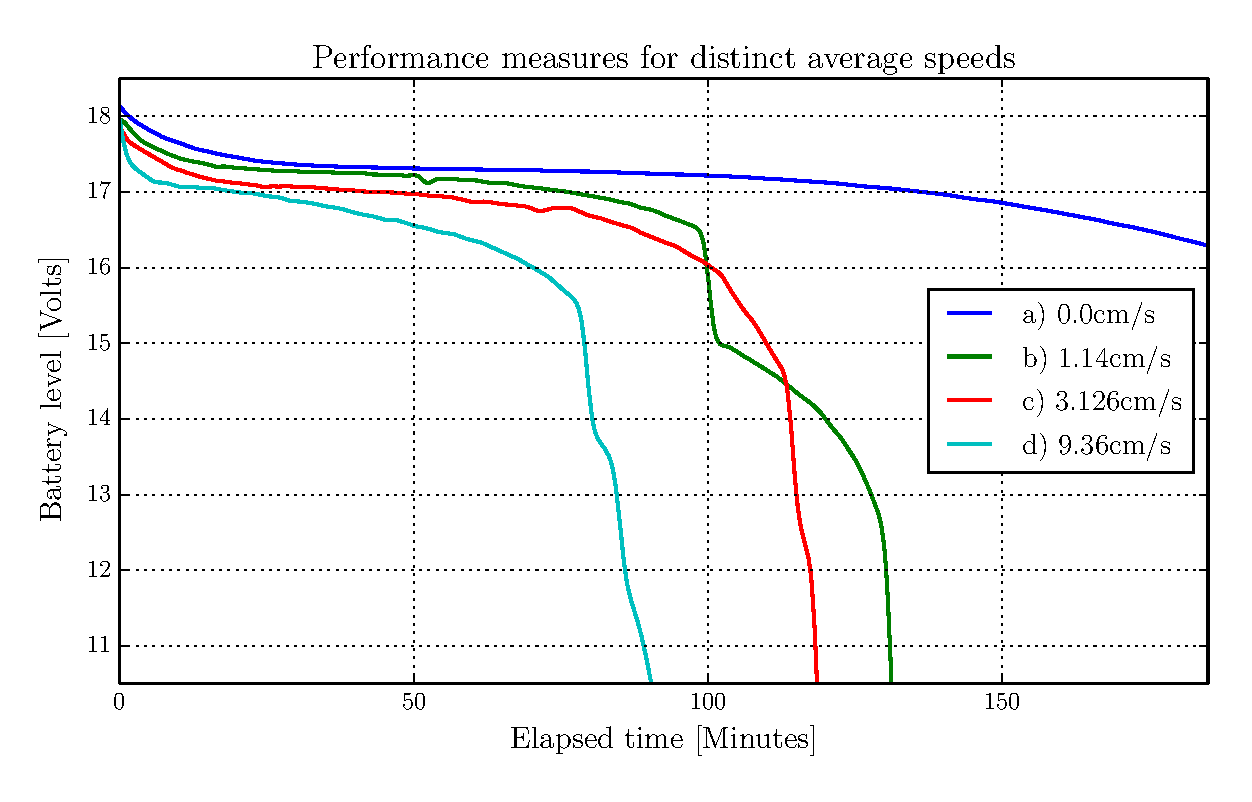
\includegraphics[width=14cm]{images/experiments/battery_performance.eps}}}
\captionFigure{Battery life measurements for distinct average speeds}
{fig:experiments/battery_performance}{
One GNBot powered by two fully-charged 9V 300mAh rechargeable batteries in series configuration was the setup used for this study. A simple obstacle-avoidance routine was used to ensure the continuous motion of the robot.
The cross of curves \emph{b)} and \emph{c)} at $t=100min$ and $t=112min$ shows the variability among the same batch of batteries, and is probably due to differences in charging history.
\emph{Operating time: a) 255min b) 131min c) 119min d) 91min}.
\emph{Distance range estimation: a) 0m b) 90.29m c) 222.26m d) 505.44m}.
}
\end{figure}



The measurements in Figure \ref{fig:experiments/battery_performance} show that servomotors do not have a linear \emph{power/performance} relationship, as they maintain a very high power consumption even at very low speeds. Using this information the search strategy can be adapted to maximize search range. This can be done, for instance, by disabling the motion of the robot when waiting for a sensor measurement to be completed.
The knowledge of various differentiated stages on the battery life is useful information that can be incorporated to trigger a decision-making event during search, to optimize the use of energy resources.
For example, abrupt changes on battery level can trigger a speed change, shutting down high consumption sensors such as the electronic nose, or altering the decision of which robot approaches a given target.
In the case of search strategies based on L\'evy walks, the motion decision extracted from the L\'evy distribution can also be modulated in real time with the battery life estimation.


\lsection{Odor sensing and detection capability}

Apart from bio-inspired energy management, sensing often requires to implement gain control in different sensory modalities to better adapt to variability in each environmental context. Modulation of the temperature of single odor sensors can serve as a virtualization of sensor arrays and it also allows for spatio-temporal encoding which can be needed for more advanced detection and classification tasks. The GNBoard is conveniently provided with the circuitry necessary to achieve this sort of adaptive modulation in odor sensing, and the functionality has been tested to perform as the original \emph{Olus} module (cf. Fig. \ref{fig:introduction/OlusAndTGS2600}).

Whilst odor sensing capability could have been evaluated as a standalone functionality, the multimodal characteristics of robotic search problems make it mandatory to have actual field measurements that demonstrate odor sensing performance. Also, as odor sensing is one of the most characteristic parts of the GNBot design, it is more than convenient to document these features.
Figure \ref{fig:experiments/roomForTests} shows the area utilized for the field odor detection experiments.

\begin{figure}[h!]
\centerline{\mbox{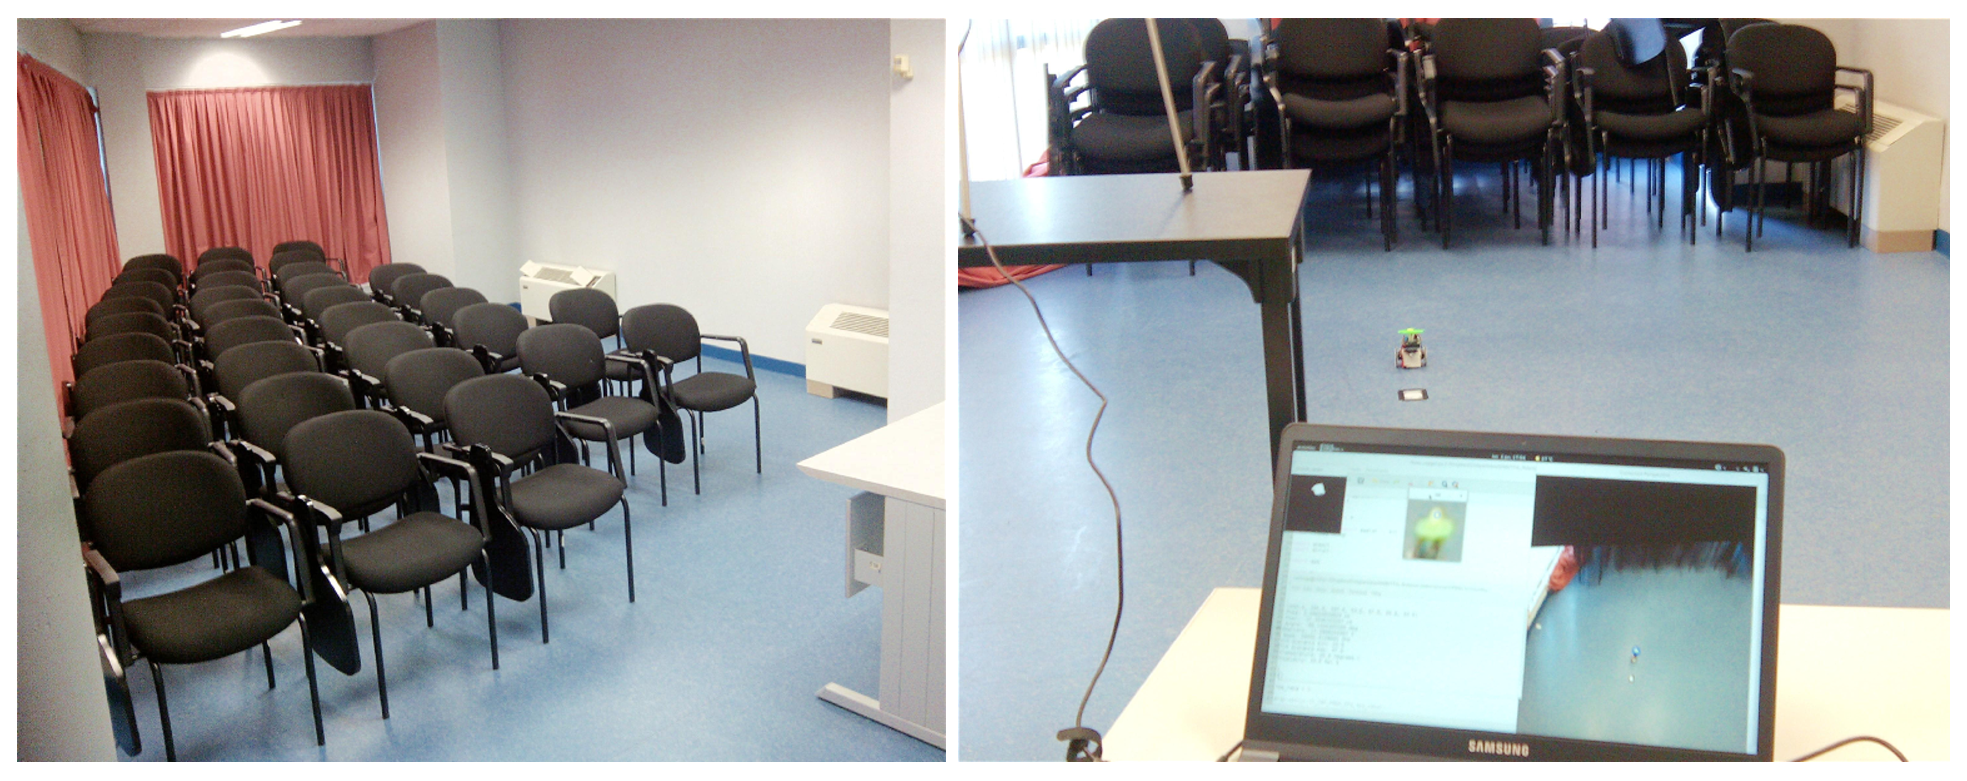
\includegraphics[width=16cm]{images/experiments/roomForTests.eps}}}
\captionFigure{Room used for the tests (left) and an experiment in progress (right)}
{fig:experiments/roomForTests}{
The chairs were moved to the back of the room before each experiment in order to have free space. Also, the air conditioning system was turned off and all windows were closed to minimize air flow. The picture on the right shows the robot approaching an odor source while the computer-vision algorithm tracks the position of the on-board visual marker.
}
\end{figure}


As each search problem can have a different definition of the characteristics of an odor source, the platform validation tests were performed for two different odor source types (shown in Fig. \ref{fig:experiments/GNBot_and_odorSources}). The evaluation of various odorant targets can also serve to demonstrate the flexibility and easy reconfiguration of the sensors in the robot platform.




\begin{figure}[h!]
\centerline{\mbox{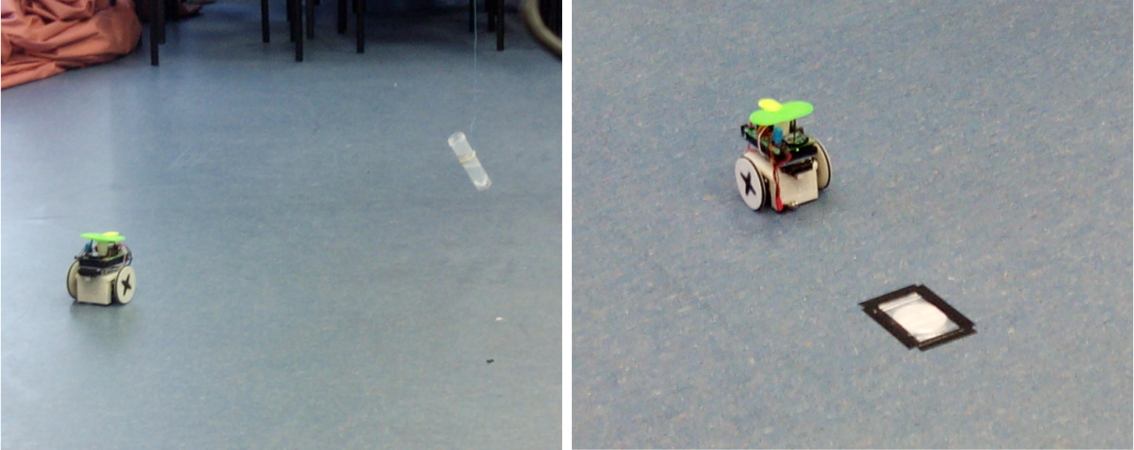
\includegraphics[width=15cm]{images/experiments/GNBot_and_odorSources.eps}}}
\captionFigure{GNBot and different odor sources}
{fig:experiments/GNBot_and_odorSources}{
The odor source on the left is an open tube containing a 50\% solution of ethanol, which is attached to the ceiling with a wire and suspended at 5cm above the robot. The low-profile target odorant on the right is based on a flat cotton pad impregnated with the same ethanol solution, and contained in a plastic bag with a circular aperture ($D=1cm$) from where the odor plume escapes.
Both odor sources were successfully detected by the GNBot, but the one on the right panel produced more repeatable results as the effect is much more local.
}
\end{figure}








\begin{figure}[h!]
\centerline{\mbox{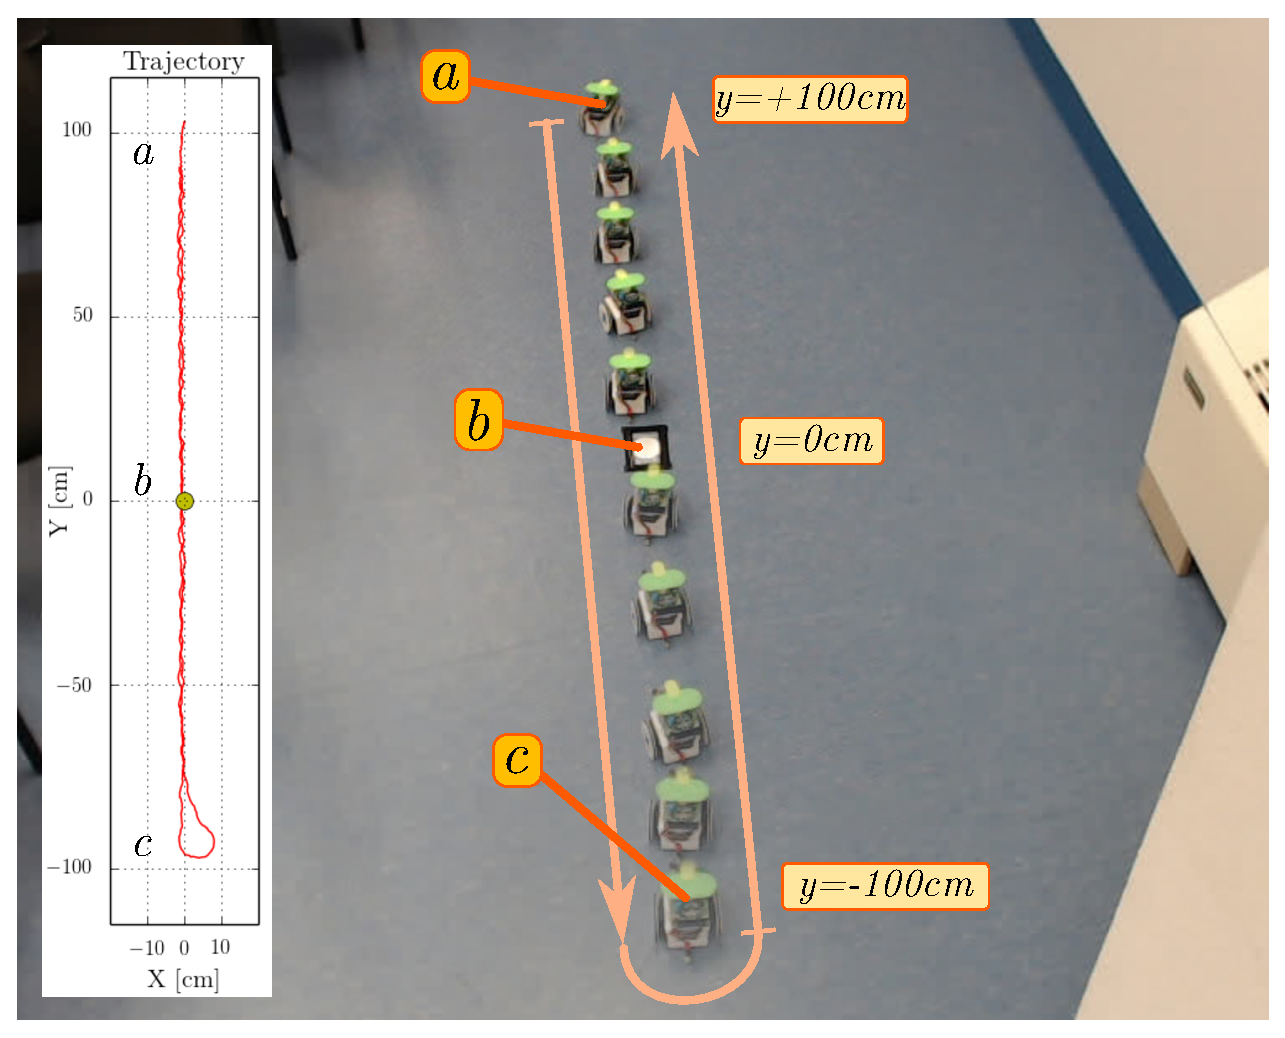
\includegraphics[width=13.5cm]{images/experiments/linearOdorMap.eps}}}
\captionFigure{Closed-loop robot trajectory over an odor source}
{fig:experiments/linearOdorMap}{
The odor source is adhered to the center of the test area \emph{(b)}.
For the target characterization, the robot performs two passes in opposite directions ($a \rightarrow b \rightarrow c$ and $c \rightarrow b \rightarrow a$). The developed navigation software autonomously commands the robot, closing the control loop with the incorporation of feedback from the visual marker tracking algorithm.
The position of the robot and all sensor measurements are logged in the computer in real time ($T=100ms$).
}
\end{figure}



In order to validate the odor sensing functionality, the decision was to perform basic tests to determine the correlation among the variables \emph{distance to an odor source} and \emph{perceived odor intensity}.
For that purpose, the autonomous navigation capacity of the GNBot was used to execute controlled linear approaches to the odor sources. Figure \ref{fig:experiments/linearOdorMap} describes the methodology of the experiment.


\vspace{-0.3cm}

\subsection{Vision-based robot localization system accuracy}

\vspace{-0.3cm}

Figure \ref{fig:experiments/linearOdorMap} can also be used to ilustrate the autonomous positioning capacity of the developed platform. A camera observing the area of the experiment is controlled by the central computer, where a machine-vision algorithm evaluates the position of each robot in the test environment.
The vision-based system has been possible since high resolution cameras have become low-cost and widely available. The precision in the position and angle measurements is better than $\pm 5cm$, which is quite acceptable, specially when compared to the size of the robots ($10$x$10cm$).
This resolution should be enough for most search algorithm implementations. The system is also highly scalable: placing multiple cameras in the ceiling would allow to monitor larger surfaces without too much overhead in cost.



\vspace{-0.3cm}

\subsection{Odor detection results}

\vspace{-0.3cm}

Characterization results for a low-profile odor source are shown in Figure \ref{fig:experiments/odor_sensor_measurements}.
\begin{figure}[h!]
\centerline{\mbox{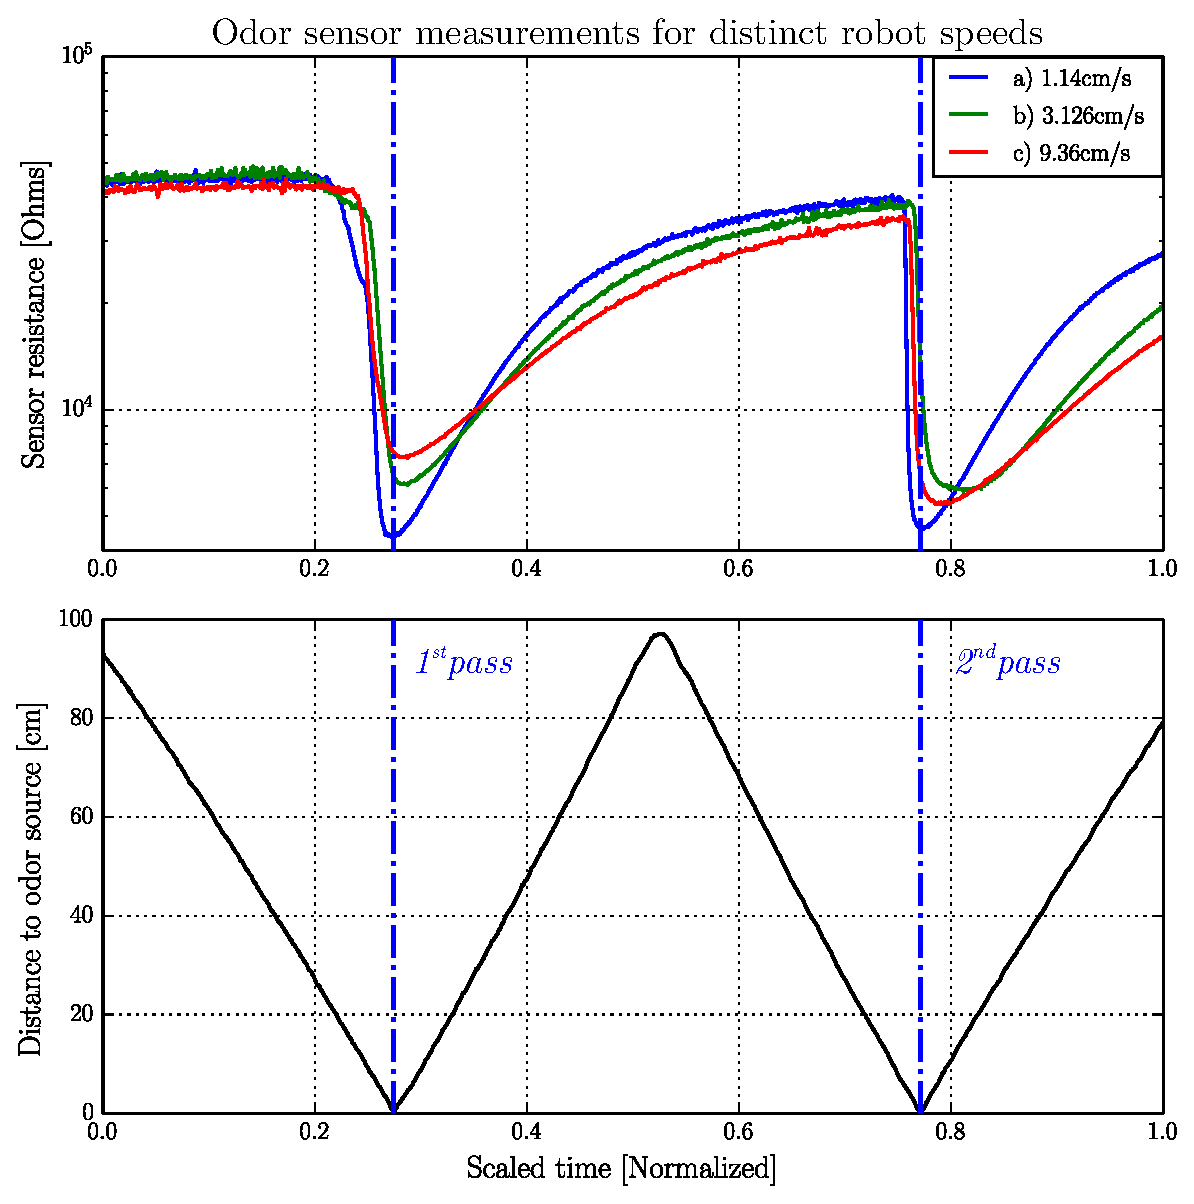
\includegraphics[width=12.5cm]{images/experiments/odor_sensor_measurements.eps}}}
\captionFigure{Odor sensor measurements for distinct robot approximation speeds}
{fig:experiments/odor_sensor_measurements}{
Sensor resistance is shown in the top panel, and the actual euclidean distance to the odorant is represented in the bottom.
For the data generation, the robot performs two passes right over the odor source, as shown in Fig. \ref{fig:experiments/linearOdorMap}.
The TGS-2600 gas sensor mounted on board the GNBot works as a resistance whose value varies in relation with the perceived odor intensity.
A reduction of resistance indicates the detection of a significative amount of odorant molecules in air. That way it is possible to identify the presence of an odor source as a falling edge in the resistance of the odor sensor, or with a simple threshold detector (i.e. $R<10k\Omega$).
The double pass of the robot over the odorant allows to determine the hysteresis in sensibility, which is related to the delay needed for normal operation after the saturation of the sensor.
}
\end{figure}
It can be appreciated that odor detection begins for the three cases at around $20cm$ from the odor source, which is the effective range that could be incorporated in search strategies.
The initial hypothesis was that for higher robot velocities the sensor response would be more abrupt, but the obtained results have shown the opposite effect: resistivity reaches lower values for more reduced speeds.
The updated hypothesis is related with the physical characteristics of the TGS-2600 odor sensor, whose sensitivity to odorant concentrations seems to become intensified for longer exposure periods.
Thus, it would be possible to modulate the localization algorithms to adjust the detection threshold according to the velocity of the robot, in order to maximize sensitivity even at high speeds.




Further odor detection tests are detailed in Figure \ref{fig:experiments/5x5reticularMap}. Even with the uncertainty introduced by the use of a suspended odor source rather than a low-profile one, the detection can be successfully achieved.
\begin{figure}[h!]
\centerline{\mbox{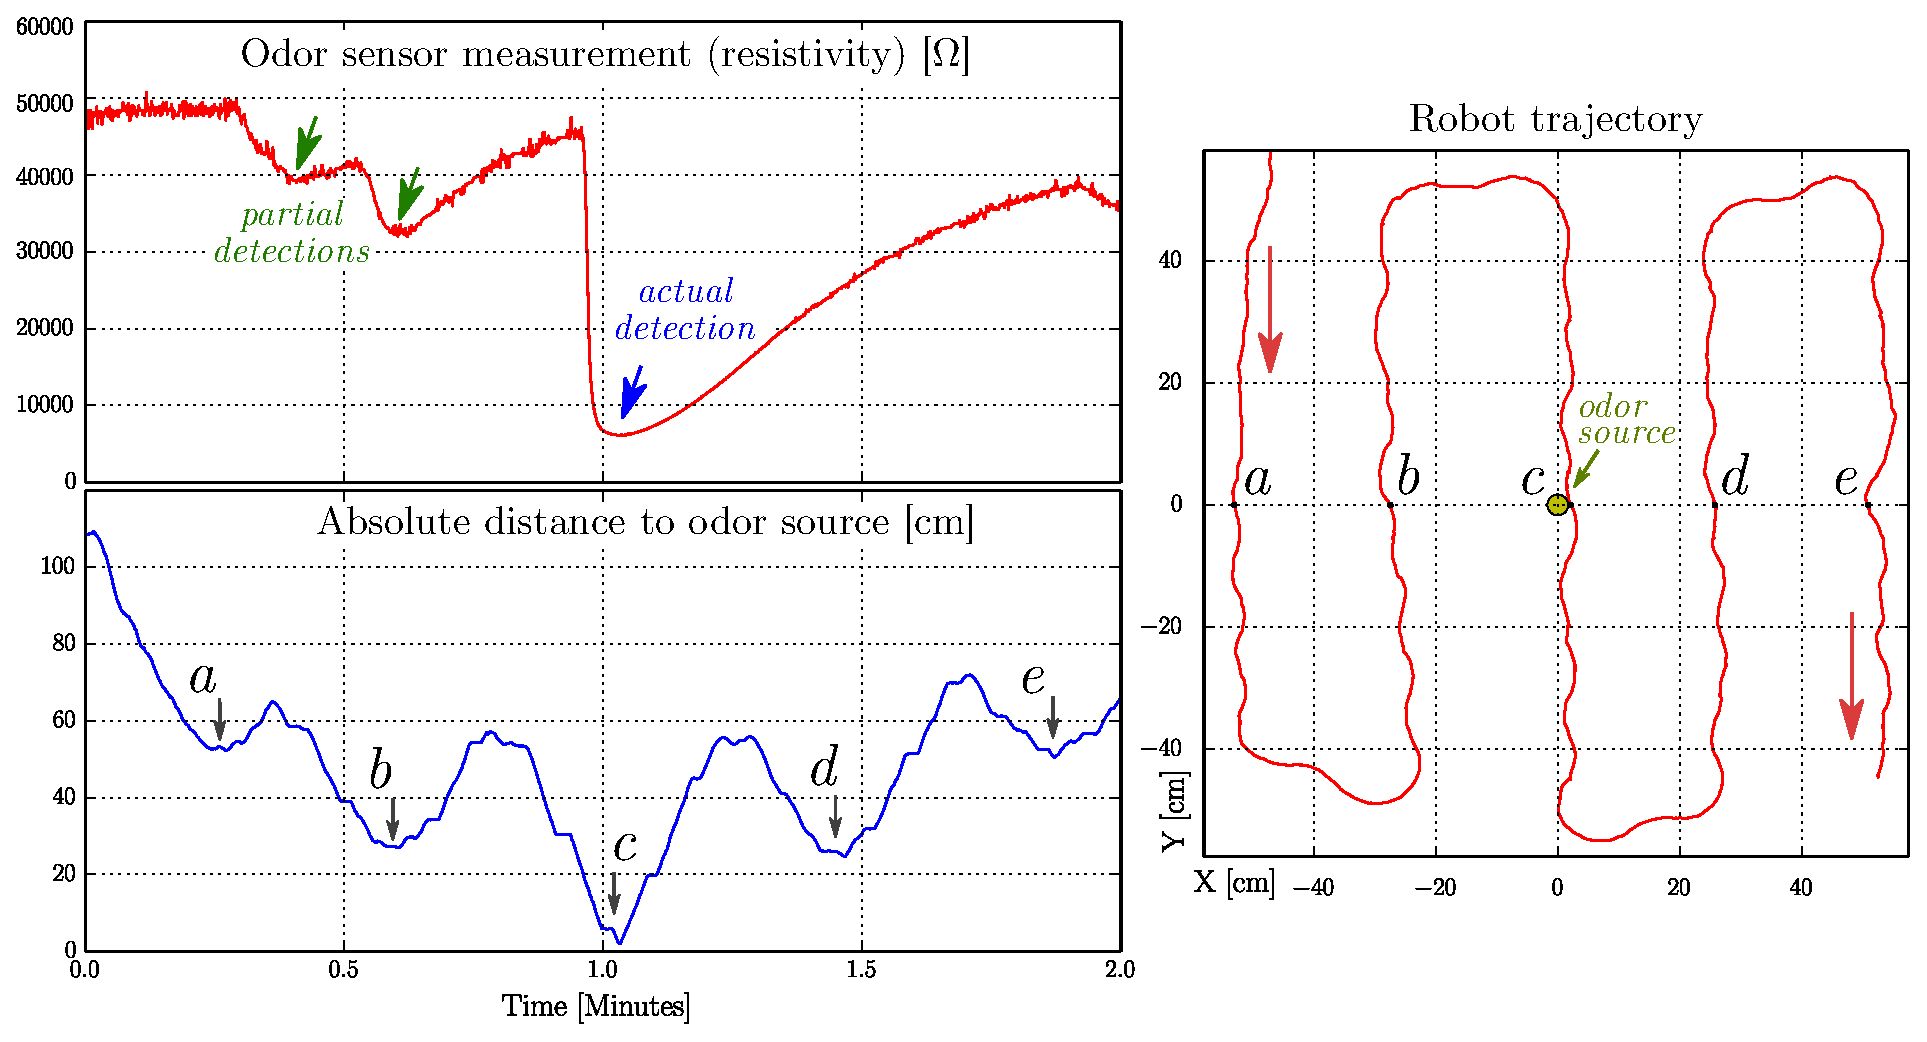
\includegraphics[width=16cm]{images/experiments/5x5reticularMap.eps}}}
\captionFigure{Odor sensor test with a 2-D trajectory}
{fig:experiments/5x5reticularMap}{
For this experiment the navigation algorithm commanded the robot to perform a zig-zag trajectory that combines a set of odor source approximations (see right panel).
The resulting measurements are shown in the left panels: the sensor response (top) and the absolute value of the distance to \emph{c} (bottom).
The suspended odor source in position \emph{c} can be perceived in the measurements even when the robot is near positions \emph{a} and \emph{b} (marked as \emph{``partial detections''}).
Simple threshold detection (i.e. $R<10k\Omega$) applied to the odor sensor response could effectively inform of the presence of the target just before the robot arrival ($t=1min$).
}
\end{figure}




The other factor that can be highlighted from measurements in Figures \ref{fig:experiments/odor_sensor_measurements} and \ref{fig:experiments/5x5reticularMap} is the recovering time -\emph{hysteresis}- of the odor sensor. Whilst the plume detection occurs quite fast, lasting only a few seconds, it can be appreciated that the saturation of the sensor lasts much longer.
For the highest speed result \emph{(c)} in Figure \ref{fig:experiments/odor_sensor_measurements} it is possible to see that in the second pass the sensor has not yet recovered from the previous detection.
This indicates that for an odor search task were multiple odor sources can appear near each other, the monitoring should be performed at slow speeds \emph{(a)} in order to avoid overlaps.



Finally, the rest of multimodal sensors present in the GNBot were also successfully tested: The frontal infra-red distance sensor provides accuracy in the centimeter scale for close-up distances ($10$-$40cm$), and the humidity and temperature sensors provide a resolution of $\pm1\%$ and $\pm0.5\,^{\circ}{\rm C}$ respectively.
The magnetometer module for the electronic compass provided an accuracy of $\pm0.1\,^{\circ}$ after calibration, though magnetic field distortion could be a problem for indoor environments as it is shown in Appendix \ref{Appendix:lightLandmarks}.
Also, wireless communication with the robots via ZigBee did not present any range related limitations and performed as expected from the manufacturer's specification.



\subsection{Easy replication of the GNBot \& four-robot team}

The replicability of the GNBot design was put to test with the creation of four identical robots (shown in Fig. \ref{fig:design/developedPlatform}). Cost was kept very low, at a total of \EUR{600} with an estimated \EUR{150} per robot.
To put the price in perspective, it is important to consider the amount of multimodal sensors present in the robot, as well as the simplistic programming layer with a resilient communication system. The robots also have a long-lasting battery life as it has been shown in \ref{sect:batterylife}.

%\begin{figure}[h!]
%\centerline{\mbox{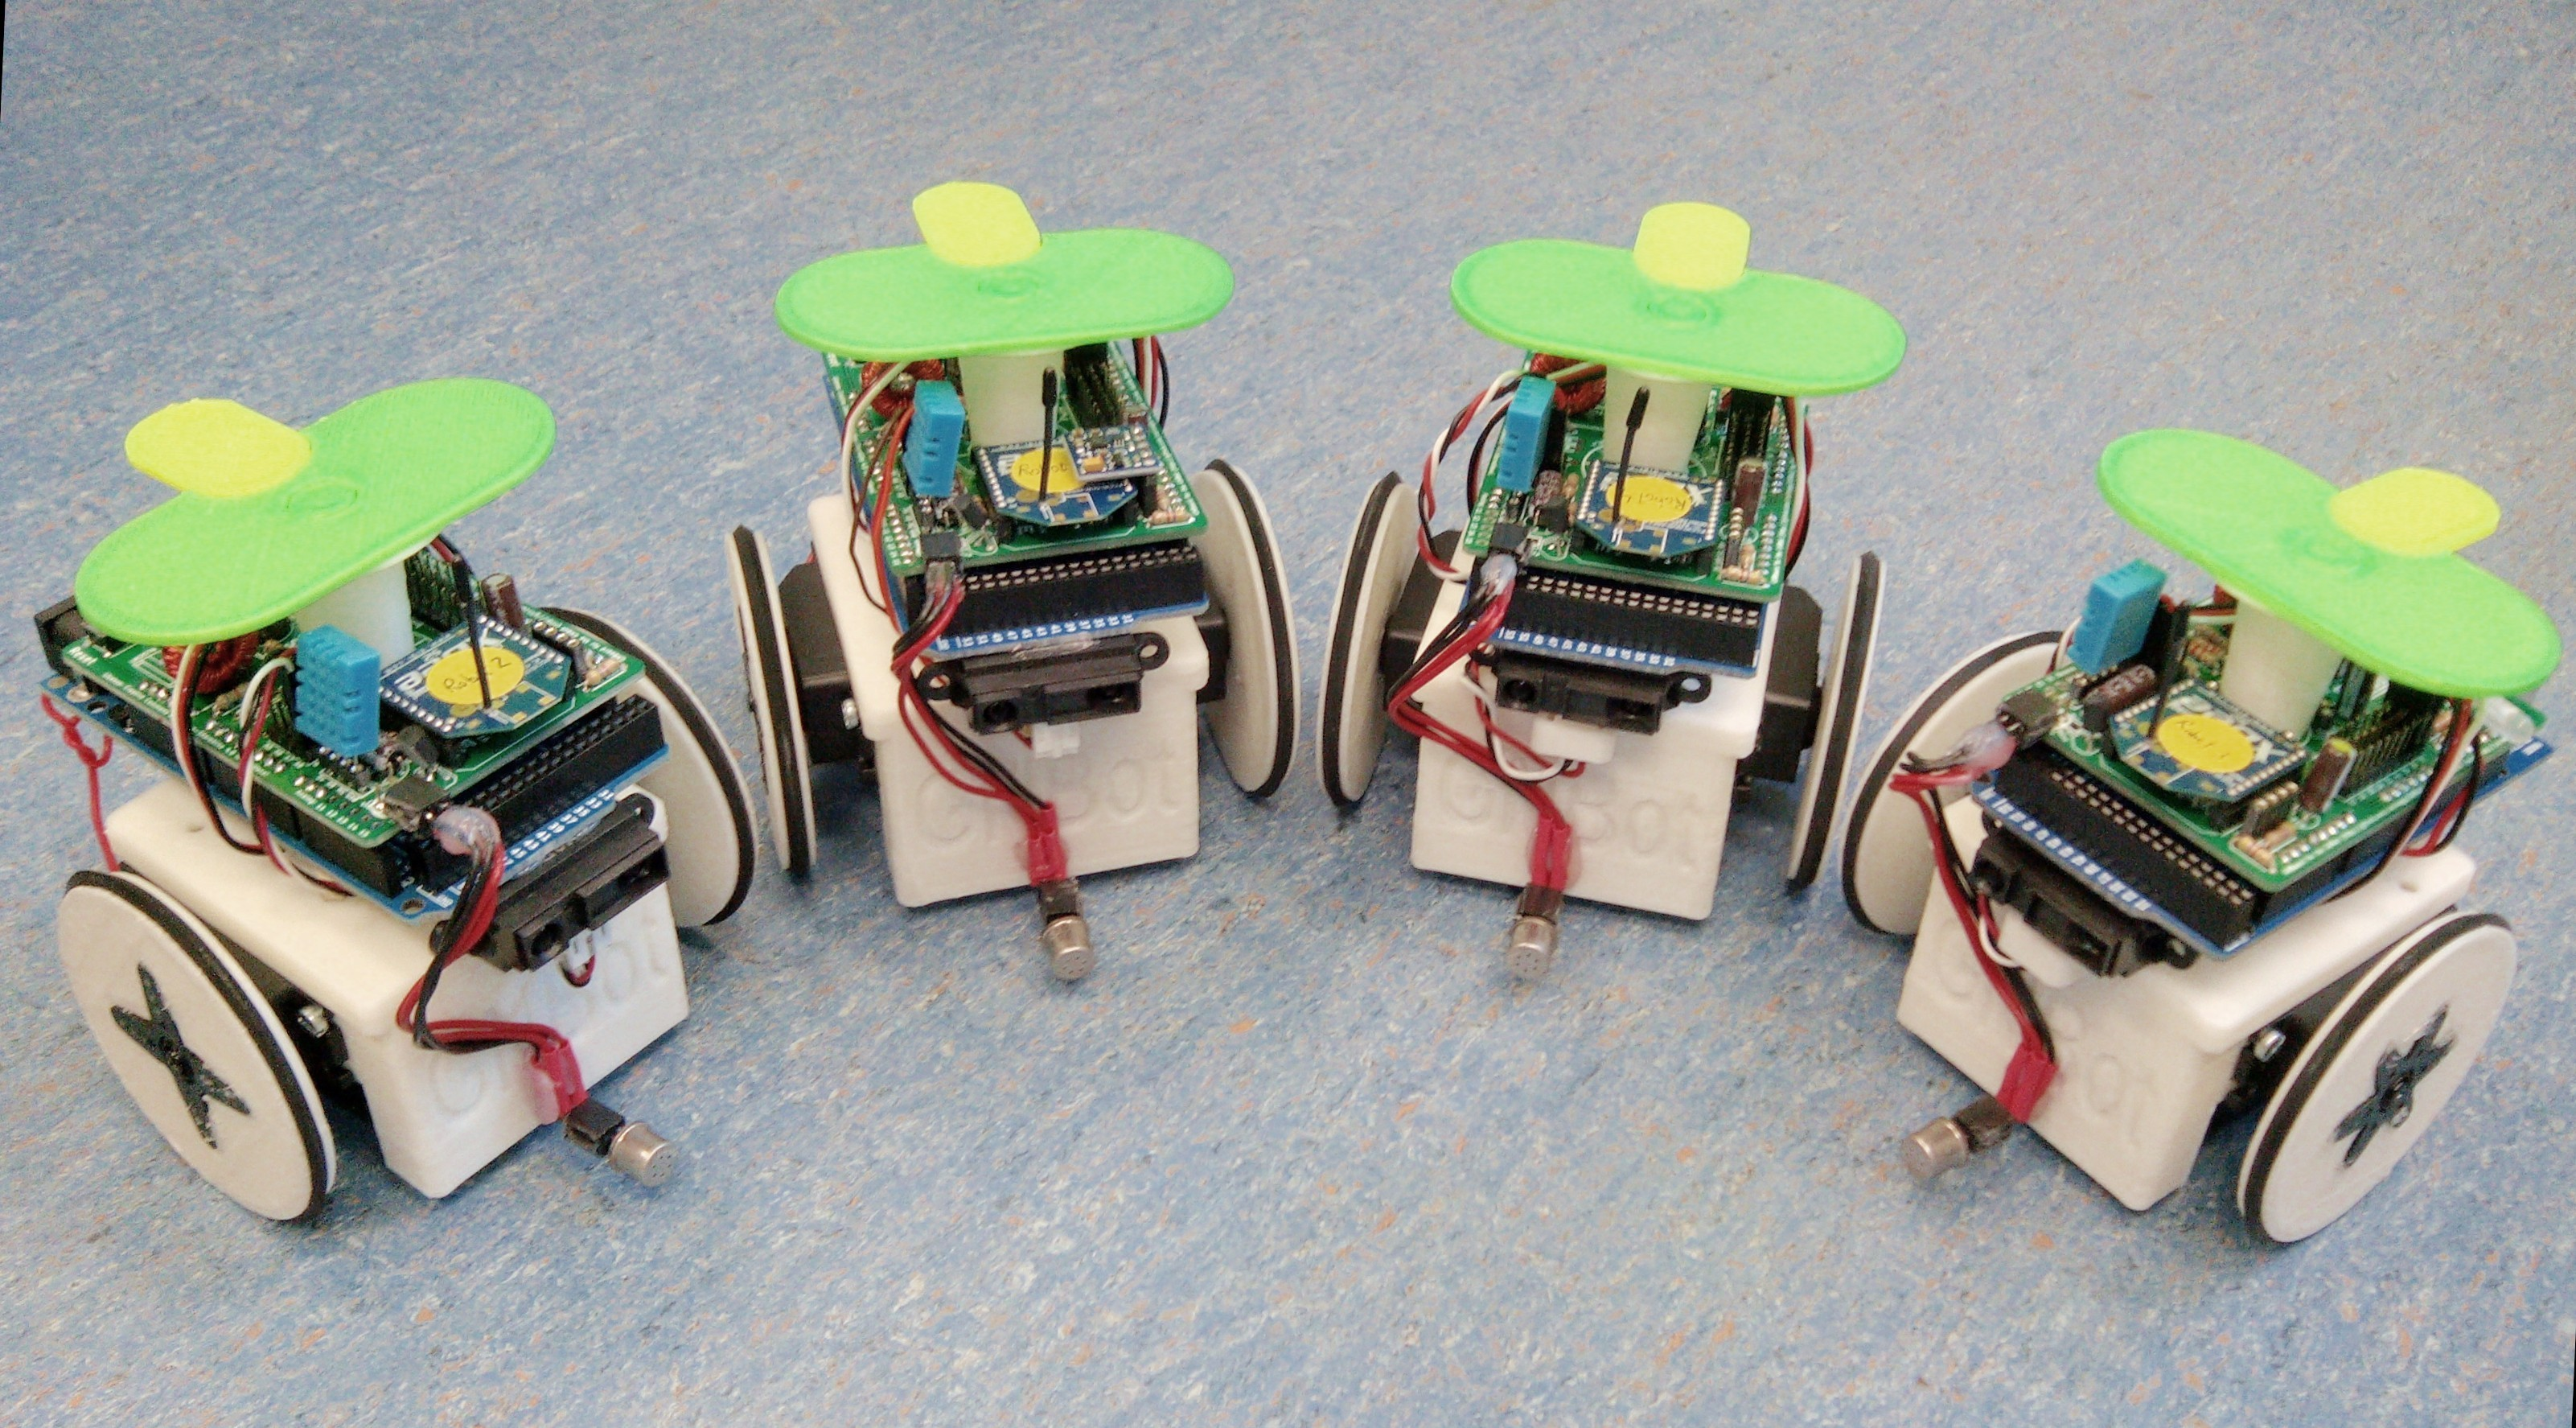
\includegraphics[width=16cm]{images/GNBot_swarm1.jpg}}}
%\captionFigure{Developed robot swarm}
%{fig:GNBot_swarm1}{
%Four identical GNBot robots equipped with a frontal TGS-2600 odor sensor.
%}
%\end{figure}

Apart from robot validation, the next scientific use for these robots
will be the implementation and real-world validation of a bio-inspired collaborative L\'{e}vy strategy developed at \emph{Grupo de Neurocomputaci\'{o}n Biol\'{o}gica} for the search of multiple odor sources in the environment.
Other strategies will be later on tested and their performance compared in a real environment, all thanks to the presence of the GNBot as a standardized robotic platform.

\newpage 

\begin{figure}[h!]
\centerline{\mbox{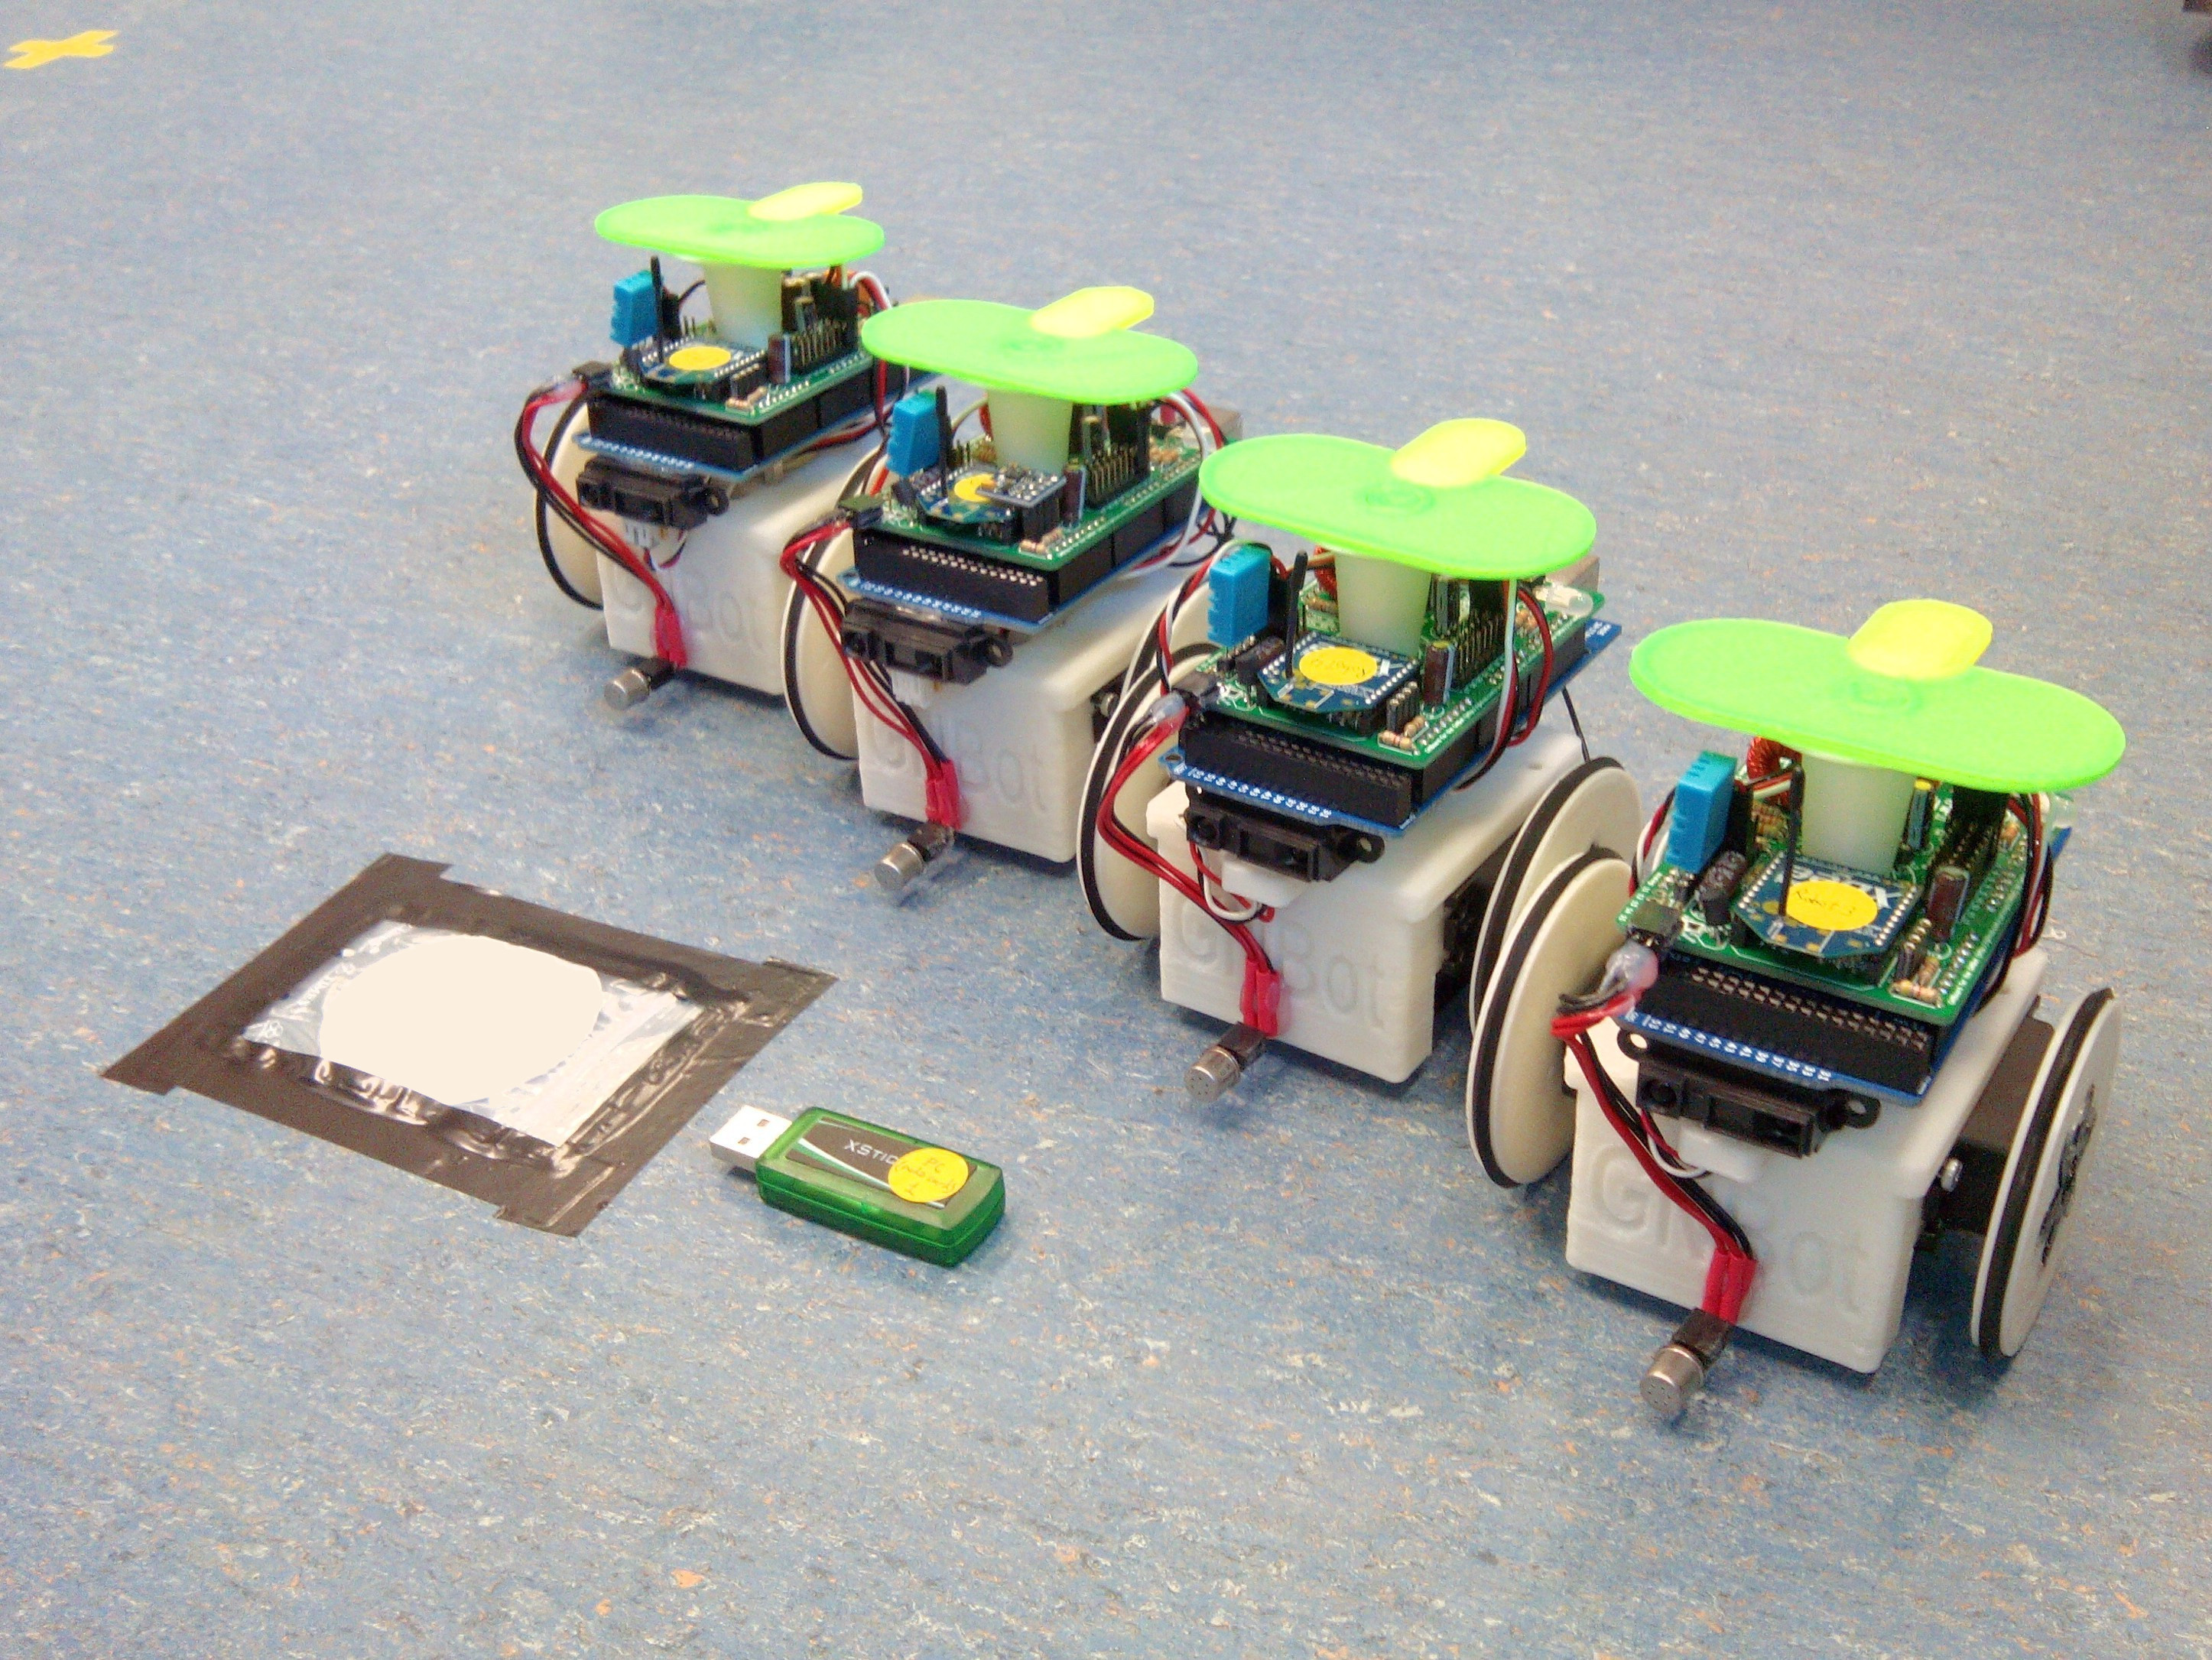
\includegraphics[width=12.5cm]{images/design/developedPlatform.jpg}}}
\captionFigure{Developed robot platform}
{fig:design/developedPlatform}{
The outcome of the project is a swarm of four remotely-controlled robots that have multimodal sensory input (perceiving light, distance, temperature, humidity and orientation with an electronic compass) and are capable of detecting odor sources such as the low-profile target shown on the left.
These robots are also energy efficient, open-source and easy to expand.
The developed system will allow the implementation of a great variety of cooperative search strategies, including those that use range information from each sensor modality with a characterization of the uncertainty of odor sources, and also the ones that use classical heuristic or brute-force approaches for search. Most importantly, the standardization of the platform could finally provide a fair base of comparison for evaluating differences in efficiency among these odor search strategies.
}\end{figure}


\newpage \thispagestyle{empty} % Página vacía



\chapter{Conclusions and future work}
\label{chap:conclusions}
\vspace{-1.5cm}


Whilst cooperative robotic search is a field that has been widely studied for many years, the use of olfactory sensors in mobile platforms seems to have raised less interest. The reason is that odor localization tasks often require cooperative strategies that have to tackle the great deal of uncertainty that can be present in the definition of the search area, the latency of odor sources, the effective detection ranges and efficiency of each sensor modality, the available resources and their estimated duration, etc.
Bio-inspired strategies that can adapt the search characteristics using context-dependent multimodal sensor integration (cf. Fig. \ref{fig:introduction/simulated_levy_walks}) could be of help in situations with such restrictions.


Among the odor monitoring services that would take benefit from research advancements on these fields are applications such as gas leak detection and localization, detection of illegal items of security concern (such as drugs or explosives), air monitoring in public spaces, environmental surveillance of large geographic areas, etc.
These particularly critical tasks are very complex to solve exclusively with man-made devices, specially since time becomes particularly relevant as the odor sources gradually fade in intensity. Still, it is often seen that these odor localization problems can be solved, as animals are used for those kind of tasks with good results.
Using bio-inspired cooperation among a large amount of robots could finally provide efficient solutions that can deal with the uncertainty and time constrains that are characteristic of those odor search problems.



The wide variety of possibilities for designing and implementing bio-inspired searches which rely on different sensory information integration and motor decision making, calls for novel flexible robotic platforms that can meet the requirements arising from handling uncertainty and resource availability within these paradigms. The approach taken by this project addressed this issue with the creation of a new robotic platform, the GNBot, an integrated solution that tries to provide maximum flexibility, scalability and reuse (cf. Fig. \ref{fig:design/GNBot_parts}). The platform has been designed to serve as a standardized method for the implementation and test of those kind of bio-inspired odor search strategies in the real world.










The developed robot has been designed to have 3D-printable pieces in combination with standardized parts, which allows an easy and fast replication. To demonstrate this, a swarm of four identical robots was assembled.
The GNBoard electronics, present on each GNBot, have also been designed to allow an easy assembly and to facilitate multi-sensor integration. By default, they can incorporate an active-sensing artificial nose, an infra-red distance sensor, temperature and humidity sensors, an electronic compass and also battery monitoring. The incorporation of the widely-available Arduino MEGA as the processor board also simplifies the implementation process.


Bidirectional wireless communication with the robots has been implemented using the ZigBee protocol, and an abstraction layer was created in order to allow higher-level programming and facilitate development. The Python programming language was used for its simplicity and for being open-source.
The centralized communication approach that has been presented (cf. Fig. \ref{fig:design/topology}) allows the abstraction of all the computational requirements to a root computer, which means that all the information of an experiment can be easily accessed in real time and each robot is effectively commanded as a peripheral.


The project has also studied various systems for the localization of robots in the search area (Section \ref{sect:realTimePositionMeasurement}).
These systems are of vital importance not only for the implementation of some search strategies, but also in the research context to allow the efficiency analysis of a given search.
A computer-vision tracking algorithm has been implemented using OpenCV to allow the use of high definition cameras for real time identification of the robot position and orientation.
The implementation has also been made open-source and could be reused for other video tracking or surveillance tasks such as neuroethological studies that involve animal position monitoring.
The also studied landmark-based systems could potentially be used in combination with computer vision and other techniques in order to improve the resolution of robot localization, and to permit the adaptation to each different real-world context. For instance, whilst the precision of GPS signals themselves cannot be sufficient for the odor localization task, integration of local landmark tracking could help to achieve the required resolution.

As the platform is easy to expand and energy efficient, it could be easily re-purposed for implementing many other mobile-sensing surveillance systems, since it allows the incorporation of the great variety of multimodal sensors that may be needed (i.e. vibration, soundwave or movement detectors, infra-red or ultra-violet target search, etc).
The implemented closed-loop way-point navigation system could also be reused for these and other tasks that involve mobile robotics.



Finally, all of the features implemented in the GNBot platform have been validated. The multimodal sensory input, including the performance of the integrated battery monitoring system, was characterized and particular interest was given to the evaluation of the robot's autonomous positioning capabilities in combination with the odor detection system.


%\vspace{-0.5cm}
\subsection*{Future work}

Appart from robot validation, the next scientific use for the assembled robots will be the implementation and real-world validation of a bio-inspired collaborative L\'{e}vy strategy that is being developed at \emph{Grupo de Neurocomputaci\'{o}n Biol\'{o}gica} for the search of multiple odor sources in the environment.
Other strategies will be later on tested and their performance compared in a real-world environment, all thanks to the presence of the GNBot as a standardized robotic platform.


Other interesting research paths could involve the incorporation of further multi-sensorial input such as directional air flow sensors. The state of the art has shown that these sensors can provide beneficial information to odor search algorithms, so it would be very interesting to integrate such sensing capabilities into the robot.
Studies that involve odor discrimination would also be possible with the developed GNBoard electronics as it allows temperature modulation for the odor sensor (cf. Fig. \ref{fig:design/artificialNose_polarization}). Another research path could be pheromone-driven robots \cite{vazquez2013integracion, Purnamadjaja07} whose interactions are made by means of odor generation and perception.


Finally, the last specified requirement was the open-source publication of the platform, and thus the development of the GNBot is kept openly acessible\footnote{\url{https://github.com/carlosgs/GNBot/}} to allow its re-use and evolution by the scientific community.


\newpage \thispagestyle{empty} % P�gina vac�a 


%\input{publications}


%\chapter*{Acknowledgements}
\vspace{-1cm}

This project is the milestone that represents the successful completion of my \emph{Degree in Telecommunication Technology and Service Engineering} at \emph{Universidad Aut\'{o}noma de Madrid}.

My four years as a student at \emph{Escuela Polit\'{e}cnica Superior}\footnote{\url{http://www.eps.uam.es/}} have given me the chance to meet very interesting people, at both a personal and professional level. All of my friends and family have been very kind and supportive from the beginning of this period, and our professors have always contributed to the highest degree of excellence in our studies.
Without all of you I surely would not be where I am sitting today.

I also want to express my most sincere gratitude to all the members at \emph{Grupo de Neurocomputaci\'{o}n Biol\'{o}gica}\footnote{\url{http://www.ii.uam.es/~gnb/}}, and in particular to my tutors \emph{Dr Pablo Varona Mart\'{i}nez} and \emph{Dr Francisco de Borja Rodr\'{i}guez}. Your excellence in research is a reference to me, and your enthusiastic guidance and constant support have been essential towards the success of this project.

Finally, I want to acknowledge the generous funding from the \emph{Spanish Ministry of Education, Culture and Sports} in the form of a \emph{2013/14 Collaboration Grant}\footnote{\url{https://sede.educacion.gob.es/catalogo-tramites/becas-ayudas-subvenciones/para-estudiar/grado/beca-colaboracion.html}}.


\vspace{0.5cm}
\hfill \emph{Carlos Garc\'{i}a-Saura}

\hfill \emph{June 2014}



\singlespacing
\addcontentsline{toc}{chapter}{\bibname}    %Agregamos al índice el capitulo de bibliografía 
\bibliographystyle{unsrt}   %plain pero ordenado en orden de aparicion en documento principal
\bibliography{robots}
\onehalfspacing

\appendix   %Indicamos que lo que viene a continuación son apéndices

%\frontmatter %Para poner los anexos en numeros romanos

%\input{anexo_presupuesto}

%\input{anexo_pliegocondiciones}

%\input{anexo_manualuso}

\chapter{Robot localization using light landmarks}
\label{Appendix:lightLandmarks}
\vspace{-1cm}


\fancyfoot[CE,CO]{APPENDIX A. LOCALIZATION USING LIGHT LANDMARKS}

This appendix summarizes the work undertaken towards a new system that would allow robot localization in a controlled environment, with the use of low-cost light sensor arrays on board each robot, in combination with purposely placed luminous landmarks.
The scenarios, data generation and techniques used for data processing are explained, and the resulting implementation is evaluated.


\subsection*{Landmark localization approach}

The proposed system would consist in stationary light sources whose position within the monitored area is known.
With a simple sensor array (shown in Fig. \ref{fig:lightLandmarks/LDR_sensor_array}), a robot would then be able to identify the direction and distance of each light source in order to infer its relative position in the environment.
As the utilized sensors were low-cost, the implementation of this technique required the calibration of the light sensor responses and the creation of adaptable models. For instance, the attenuation of light due to distance (Fig. \ref{fig:lightLandmarks/LDR_intensityVSdistance}) was modeled with exponential curve fitting in order to linearize the sensor responses.









\begin{figure}[h!]
\centerline{\mbox{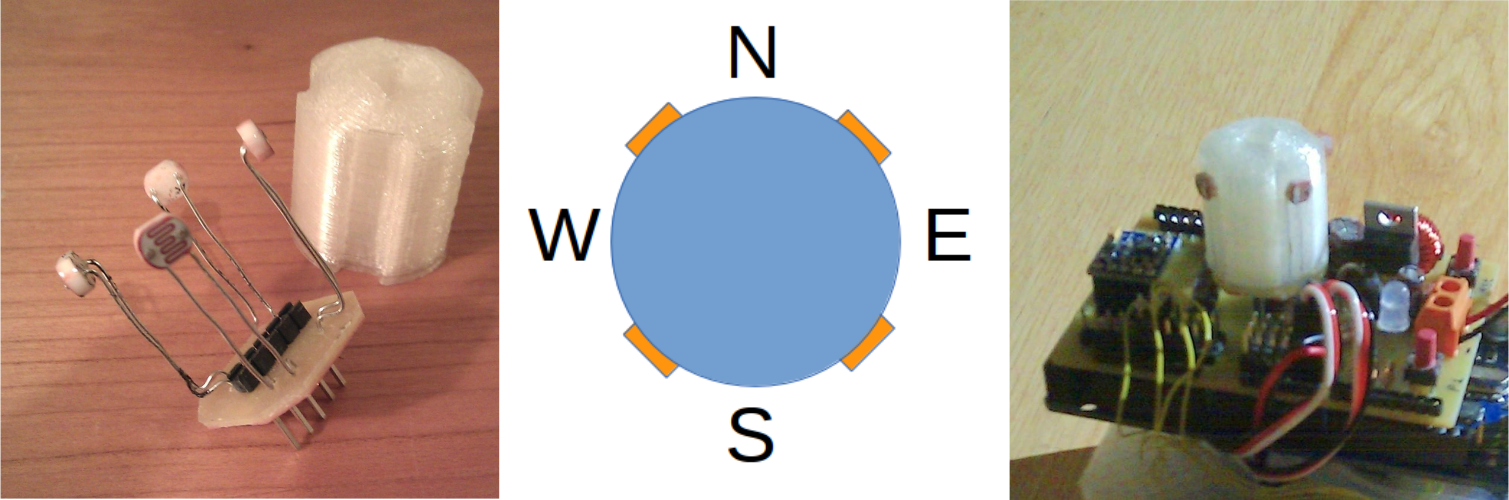
\includegraphics[width=15cm]{images/lightLandmarks/LDR_sensor_array.eps}}}
\captionFigure{Low-cost light sensor array for light-based landmark localization}
{fig:lightLandmarks/LDR_sensor_array}{
Light sensor array (left), position diagram (middle) and array mounted in a GNBot (right).
The light sensor array is made of four light-dependent resistors arranged in a ring shape. These are held in position using a 3D-printed shape designed for the purpose, and can be easily connected to the GNBoard electronics. The output is measured as a 10 bit ADC value [0-1023] that is proportional to the resistance.
}\end{figure}






\begin{figure}[h!]
\centerline{\mbox{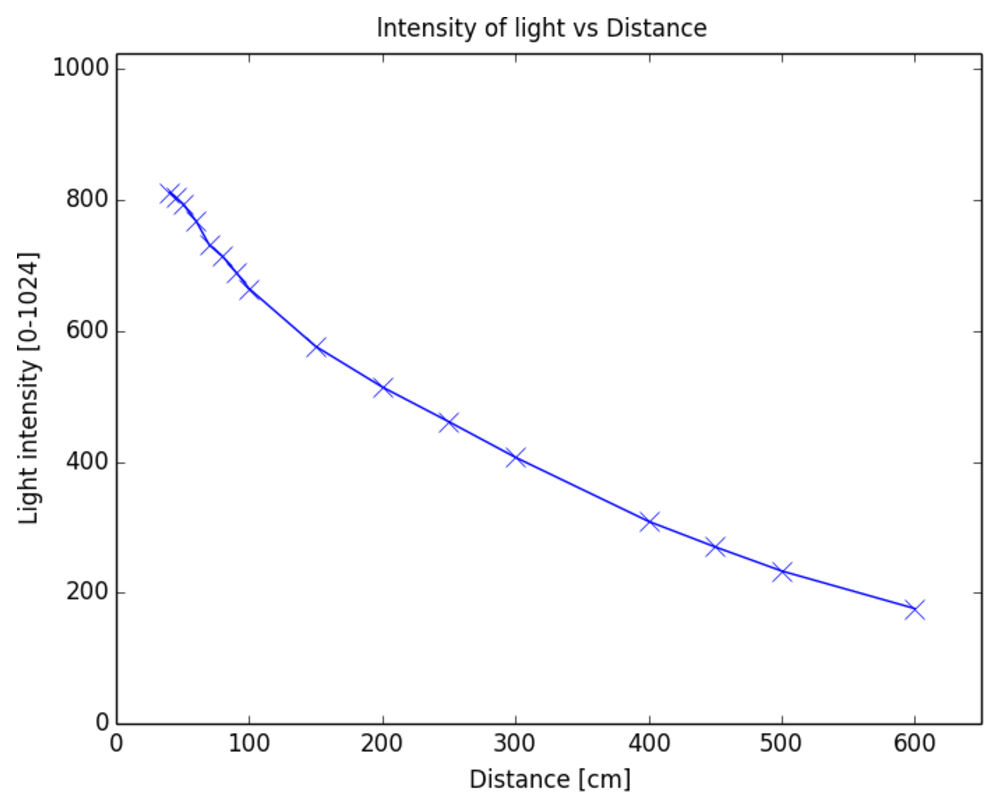
\includegraphics[width=9cm]{images/lightLandmarks/LDR_intensityVSdistance.eps}}}
\captionFigure{Response curve of the light sensors utilized}
{fig:lightLandmarks/LDR_intensityVSdistance}{
The figure shows the measured response of a light sensor at 16 different distances from a light source.
By modeling this response curve it is possible to later infer the distance of a perceived light source.
Details on the employed sensor can be found in Fig. \ref{fig:lightLandmarks/LDR_sensor_array}.
}\end{figure}







\subsubsection{Data generation for light source modeling}


The motion of the robot was restricted to be a rotation over the XY plane to simplify the initial light source modeling experiments. This decision was made since the swarm of robots would be operating in a 2-D environment. By restricting the motion to a rotation, it is possible to evaluate the light intensity measurements more easily. The experiments are described in Figure \ref{fig:lightLandmarks/GNBot_light_landmarks}.

\begin{figure}[h!]
\centerline{\mbox{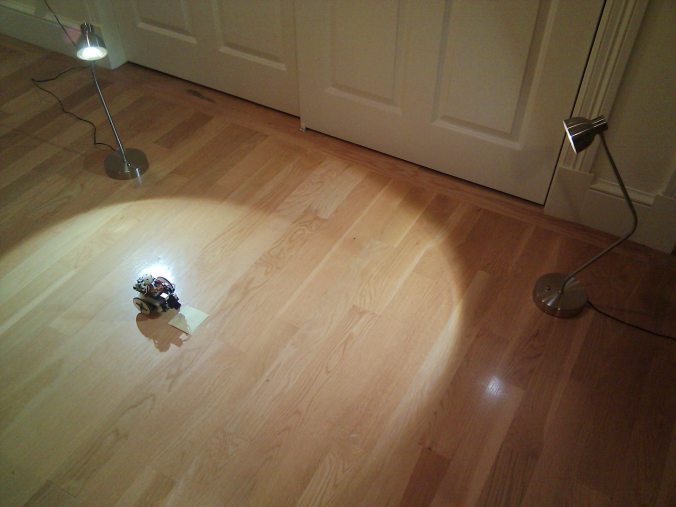
\includegraphics[width=10cm]{images/lightLandmarks/GNBot_light_landmarks.eps}}}
\captionFigure{GNBot and two light-based landmarks}
{fig:lightLandmarks/GNBot_light_landmarks}{
For the data generation, $N$ light sources were placed in the robot's operating environment. The robot was located on a known spot, where it would make M self-turns spinning at a constant speed while logging the following data:
\vspace{-0.3cm}
\begin{packed_enum}
	\item Intensity of light measured by each sensor of the array
	\item Angle of rotation of the robot measured with the electronic compass
\end{packed_enum}
\vspace{-0.3cm}
At the end, the goal was to determine the direction (angle) and distance to each of the light sources.
}\end{figure}



After some initial tests, a number of measurements were conducted. Each test was repeated both with ambient light and in the dark, with M = 3 full rotations for each experiment.
%\vspace{-0.3cm}
%\begin{packed_enum}
%	\item No light focuses
%	\item One light focus (bright) 
%	\item Two light focuses (both bright) - shown in Fig. \ref{fig:lightLandmarks/GNBot_light_landmarks}
%	\item Three light focuses (two bright, one dim)
%	\item Four light focuses (two bright, two dim)
%\end{packed_enum}
%\vspace{-0.3cm}
One light focus was added at a time, and all the parameters of the experiment (real position of each light, amount of ambient light, and all of the sensor responses) were logged in real time using a Python script.
The measurements did not have any significative noise, so no pre-filtering was required, and Matplotlib was used to represent the data (see Fig. \ref{fig:lightLandmarks/LDR_rawData_experiments}).


\begin{figure}[h!]
\centerline{\mbox{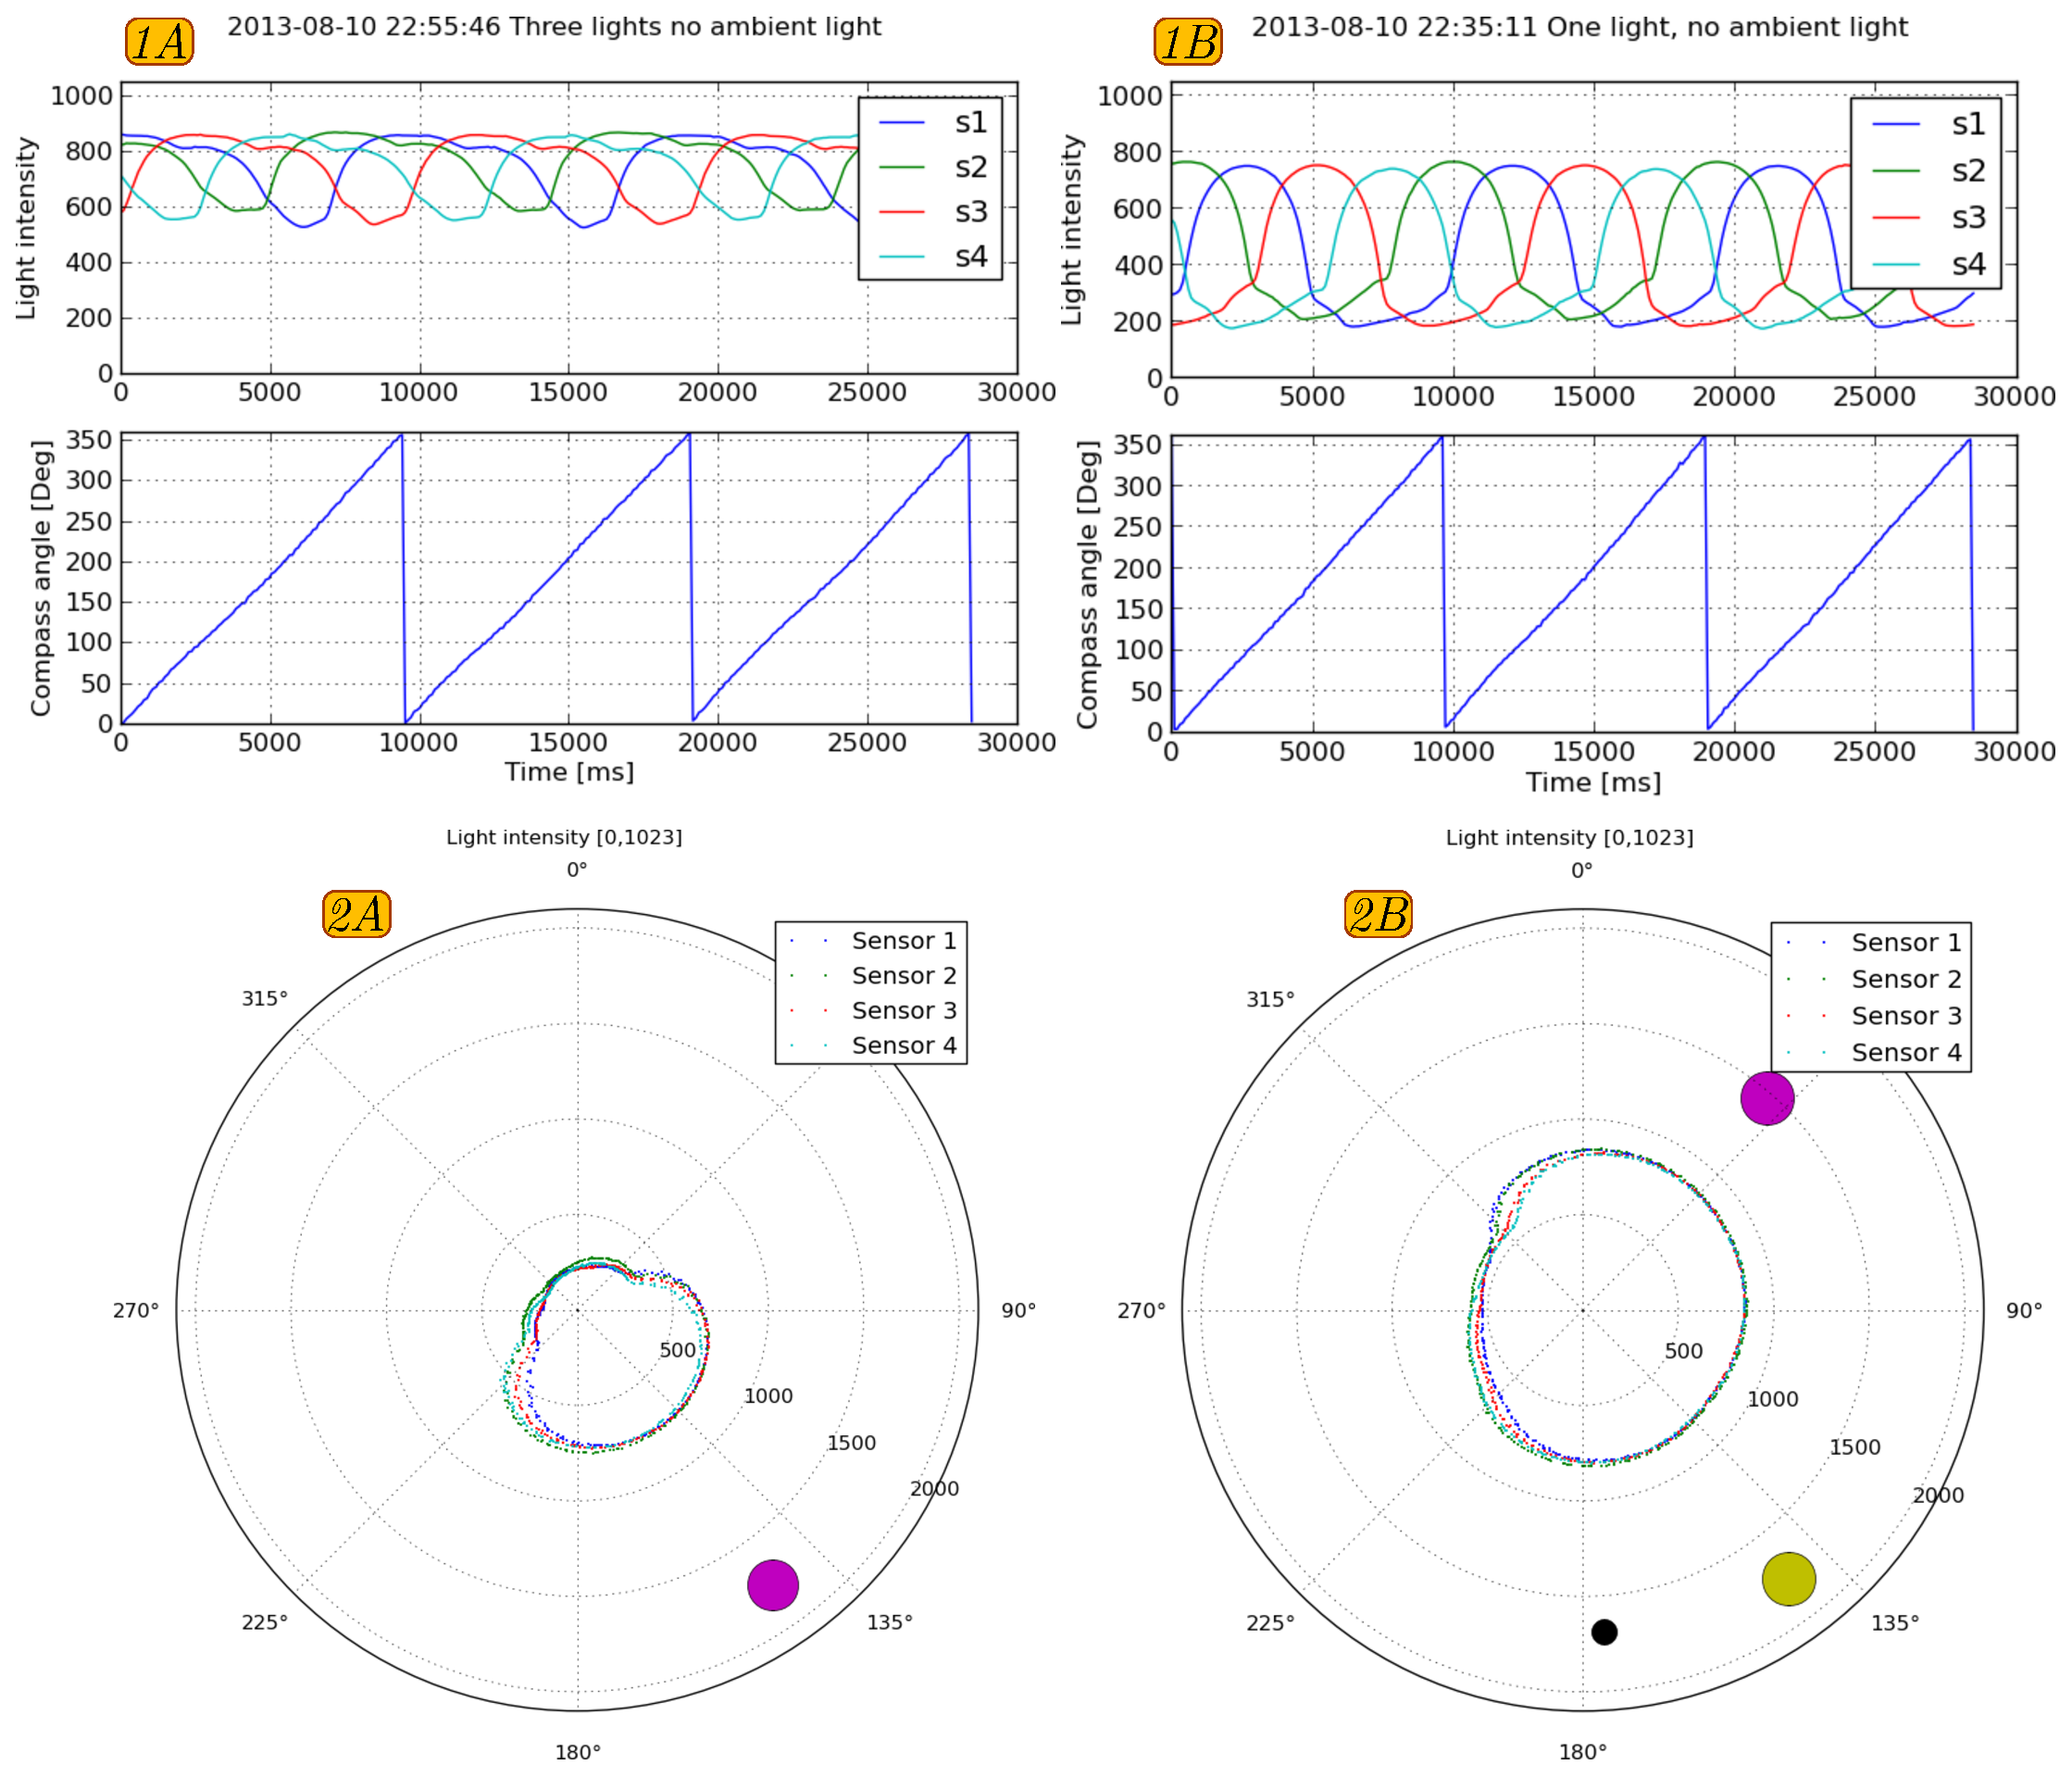
\includegraphics[width=17cm]{images/lightLandmarks/LDR_rawData_experiments.eps}}}
\captionFigure{Data from two different light landmark measurements}
{fig:lightLandmarks/LDR_rawData_experiments}{
\emph{1.A} and \emph{1.B} show the raw data from the two experiments.
\emph{2.A} and \emph{2.B} show the same data with a polar representation.
The actual position of light sources appears as colored circles.
Polar representation was preferred since the temporal dimension did not provide significative information as light sources were time invariant.
}\end{figure}




\subsubsection{Modeling the light-based landmarks}

As the intensity values are recording among an orientation measure (in degrees), the datapoints presented periodicity and thus required special polar treatment (see Fig. \ref{fig:lightLandmarks/LDR_polyfitVSfft}).




%\subsubsubsection{Polar data sampling and smoothing}


\begin{figure}[h!]
\centerline{\mbox{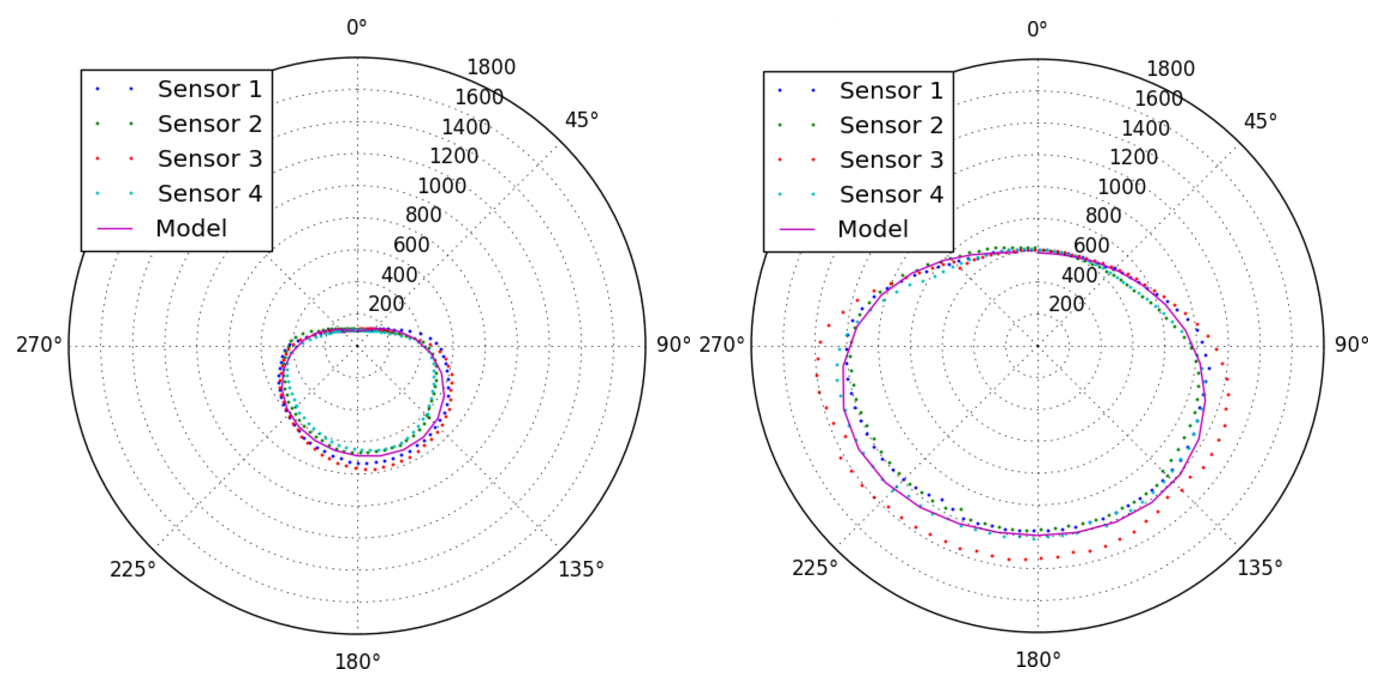
\includegraphics[width=15cm]{images/lightLandmarks/LDR_polyfitVSfft.eps}}}
\captionFigure{Smoothing the polar data using FFT low-pass filtering}
{fig:lightLandmarks/LDR_polyfitVSfft}{
The panels show the application of an FFT low-pass filter to smooth light data measurements that are polar. As a first approach, polynomial data curve fitting was used for this task, but the resulted curves presented discontinuities. The periodicity properties of FFT provided continuous results that were more adequate for the task.
}\end{figure}



%\subsubsection{Particle filtering}

%\begin{figure}[h!]
%\centerline{\mbox{\includegraphics[width=15cm]{images/placeholder.eps}}}
%\captionFigure{Diagram showing how the light-landmark localization works}
%{fig:lightLandmarks/}{
%Description
%}\end{figure}



%\subsubsection{Light landmark localization results}


After examining all the resulting data, the selected approach was to use a single light landmark (instead of multiple lights) and to incorporate measurements from both the light sensor array and the electronic compass on board the GNBot.
By measuring its global orientation and the perceived direction to the light source, the robot could then infer its relative position to the landmark (see Fig. \ref{fig:lightLandmarks/LDR_particleFilter_results}).


\begin{figure}[h!]
\centerline{\mbox{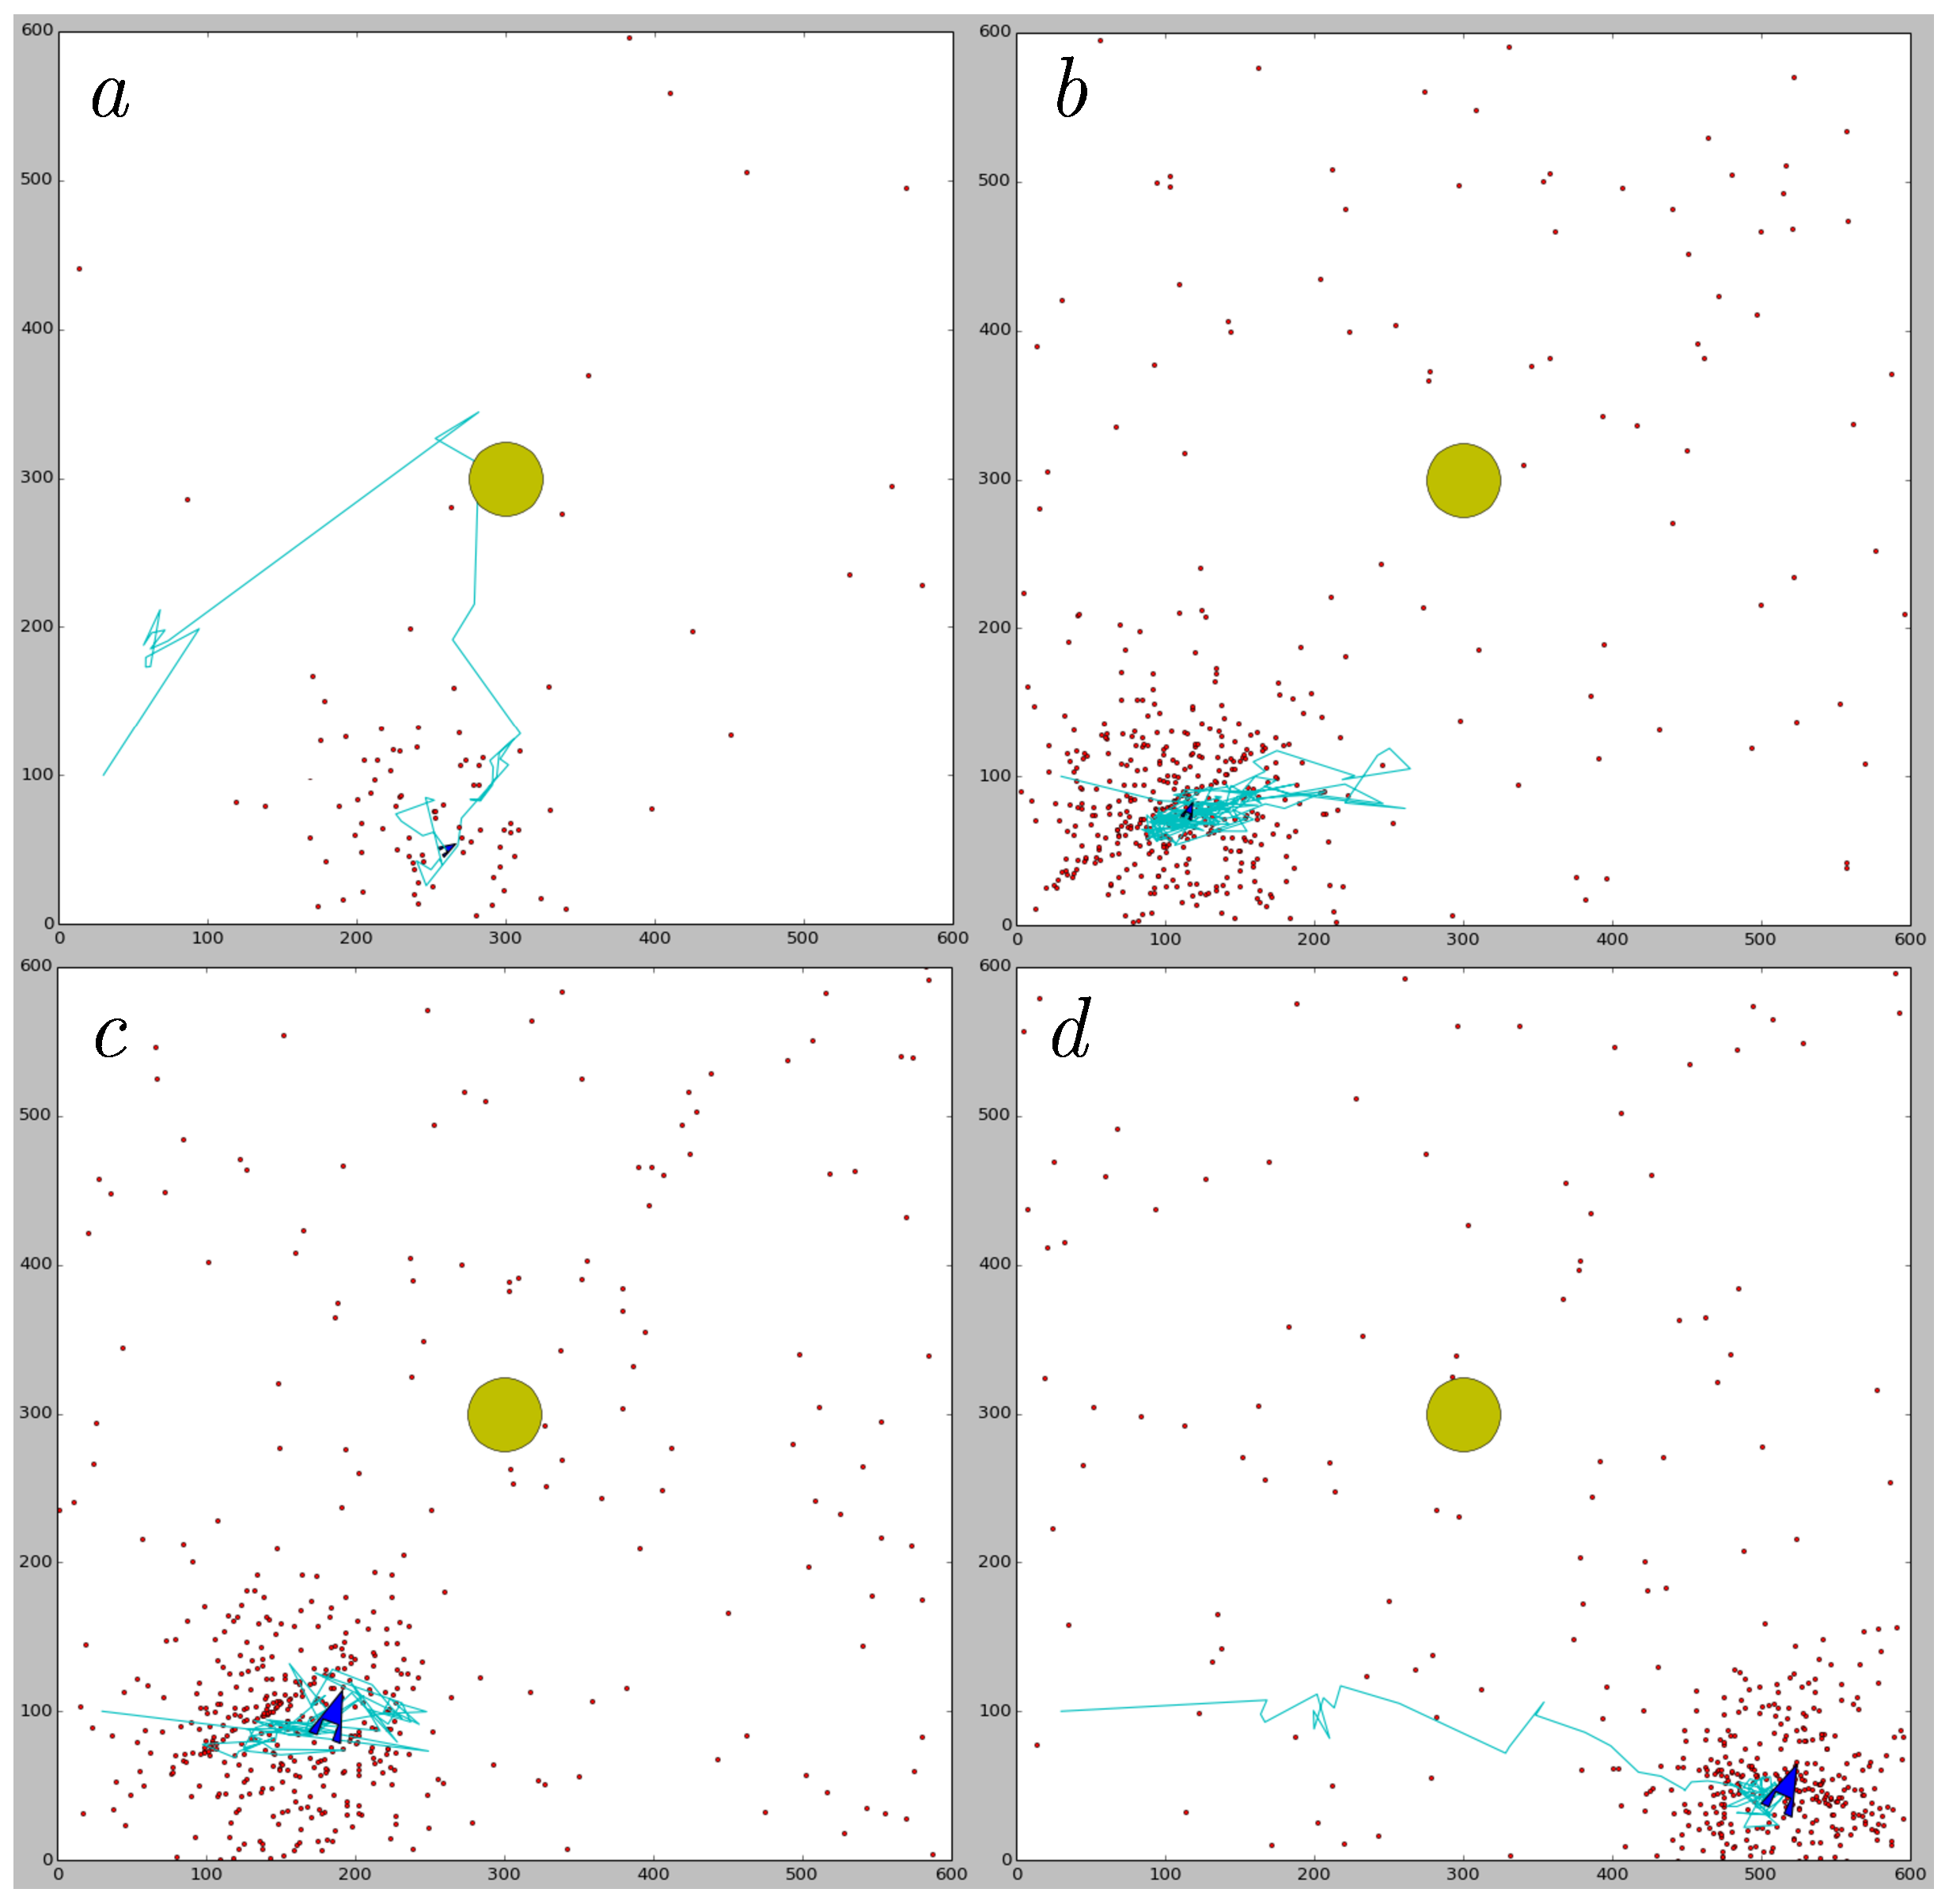
\includegraphics[width=14cm]{images/lightLandmarks/LDR_particleFilter_results.eps}}}
\captionFigure{2-D position estimation based on a light landmark}
{fig:lightLandmarks/LDR_particleFilter_results}{
The panels show data from various real robot localization experiments involving a particle filter in combination with measurements from the light sensor array and the electronic compass. Scale is in centimeters. The results have a lot of noise, because of the poor stability of the magnetic field measurement indoors.
}
\end{figure}

The implemented system performed with reasonable accuracy in simulations, but the electronic compass did not perform as expected and made the real world implementation very unreliable (specially when compared with the accuracy of the vision-based tracking system implemented in Section \ref{sect:visionBasedLocalization}).
The problem was that building floors usually have metal structures underneath, so the magnetic field is particularly distorted at low heights. Since the robots are quite low-profile, the magnetometer is then too strongly influenced by the presence of metals in the floor to allow proper robot localization.

Though, this approach for light landmark modeling and localization could be of interest for certain outdoor situations such as underwater positioning, where the light from the Sun does not create much interference.


\newpage \thispagestyle{empty} % Pagina vacia 



\fancyfoot[CE,CO]{\leftmark}



\chapter{GNBoard design schematics and layout}
\label{Appendix:circuits}
\vspace{-1cm}


\begin{figure}[h!]
\centerline{\mbox{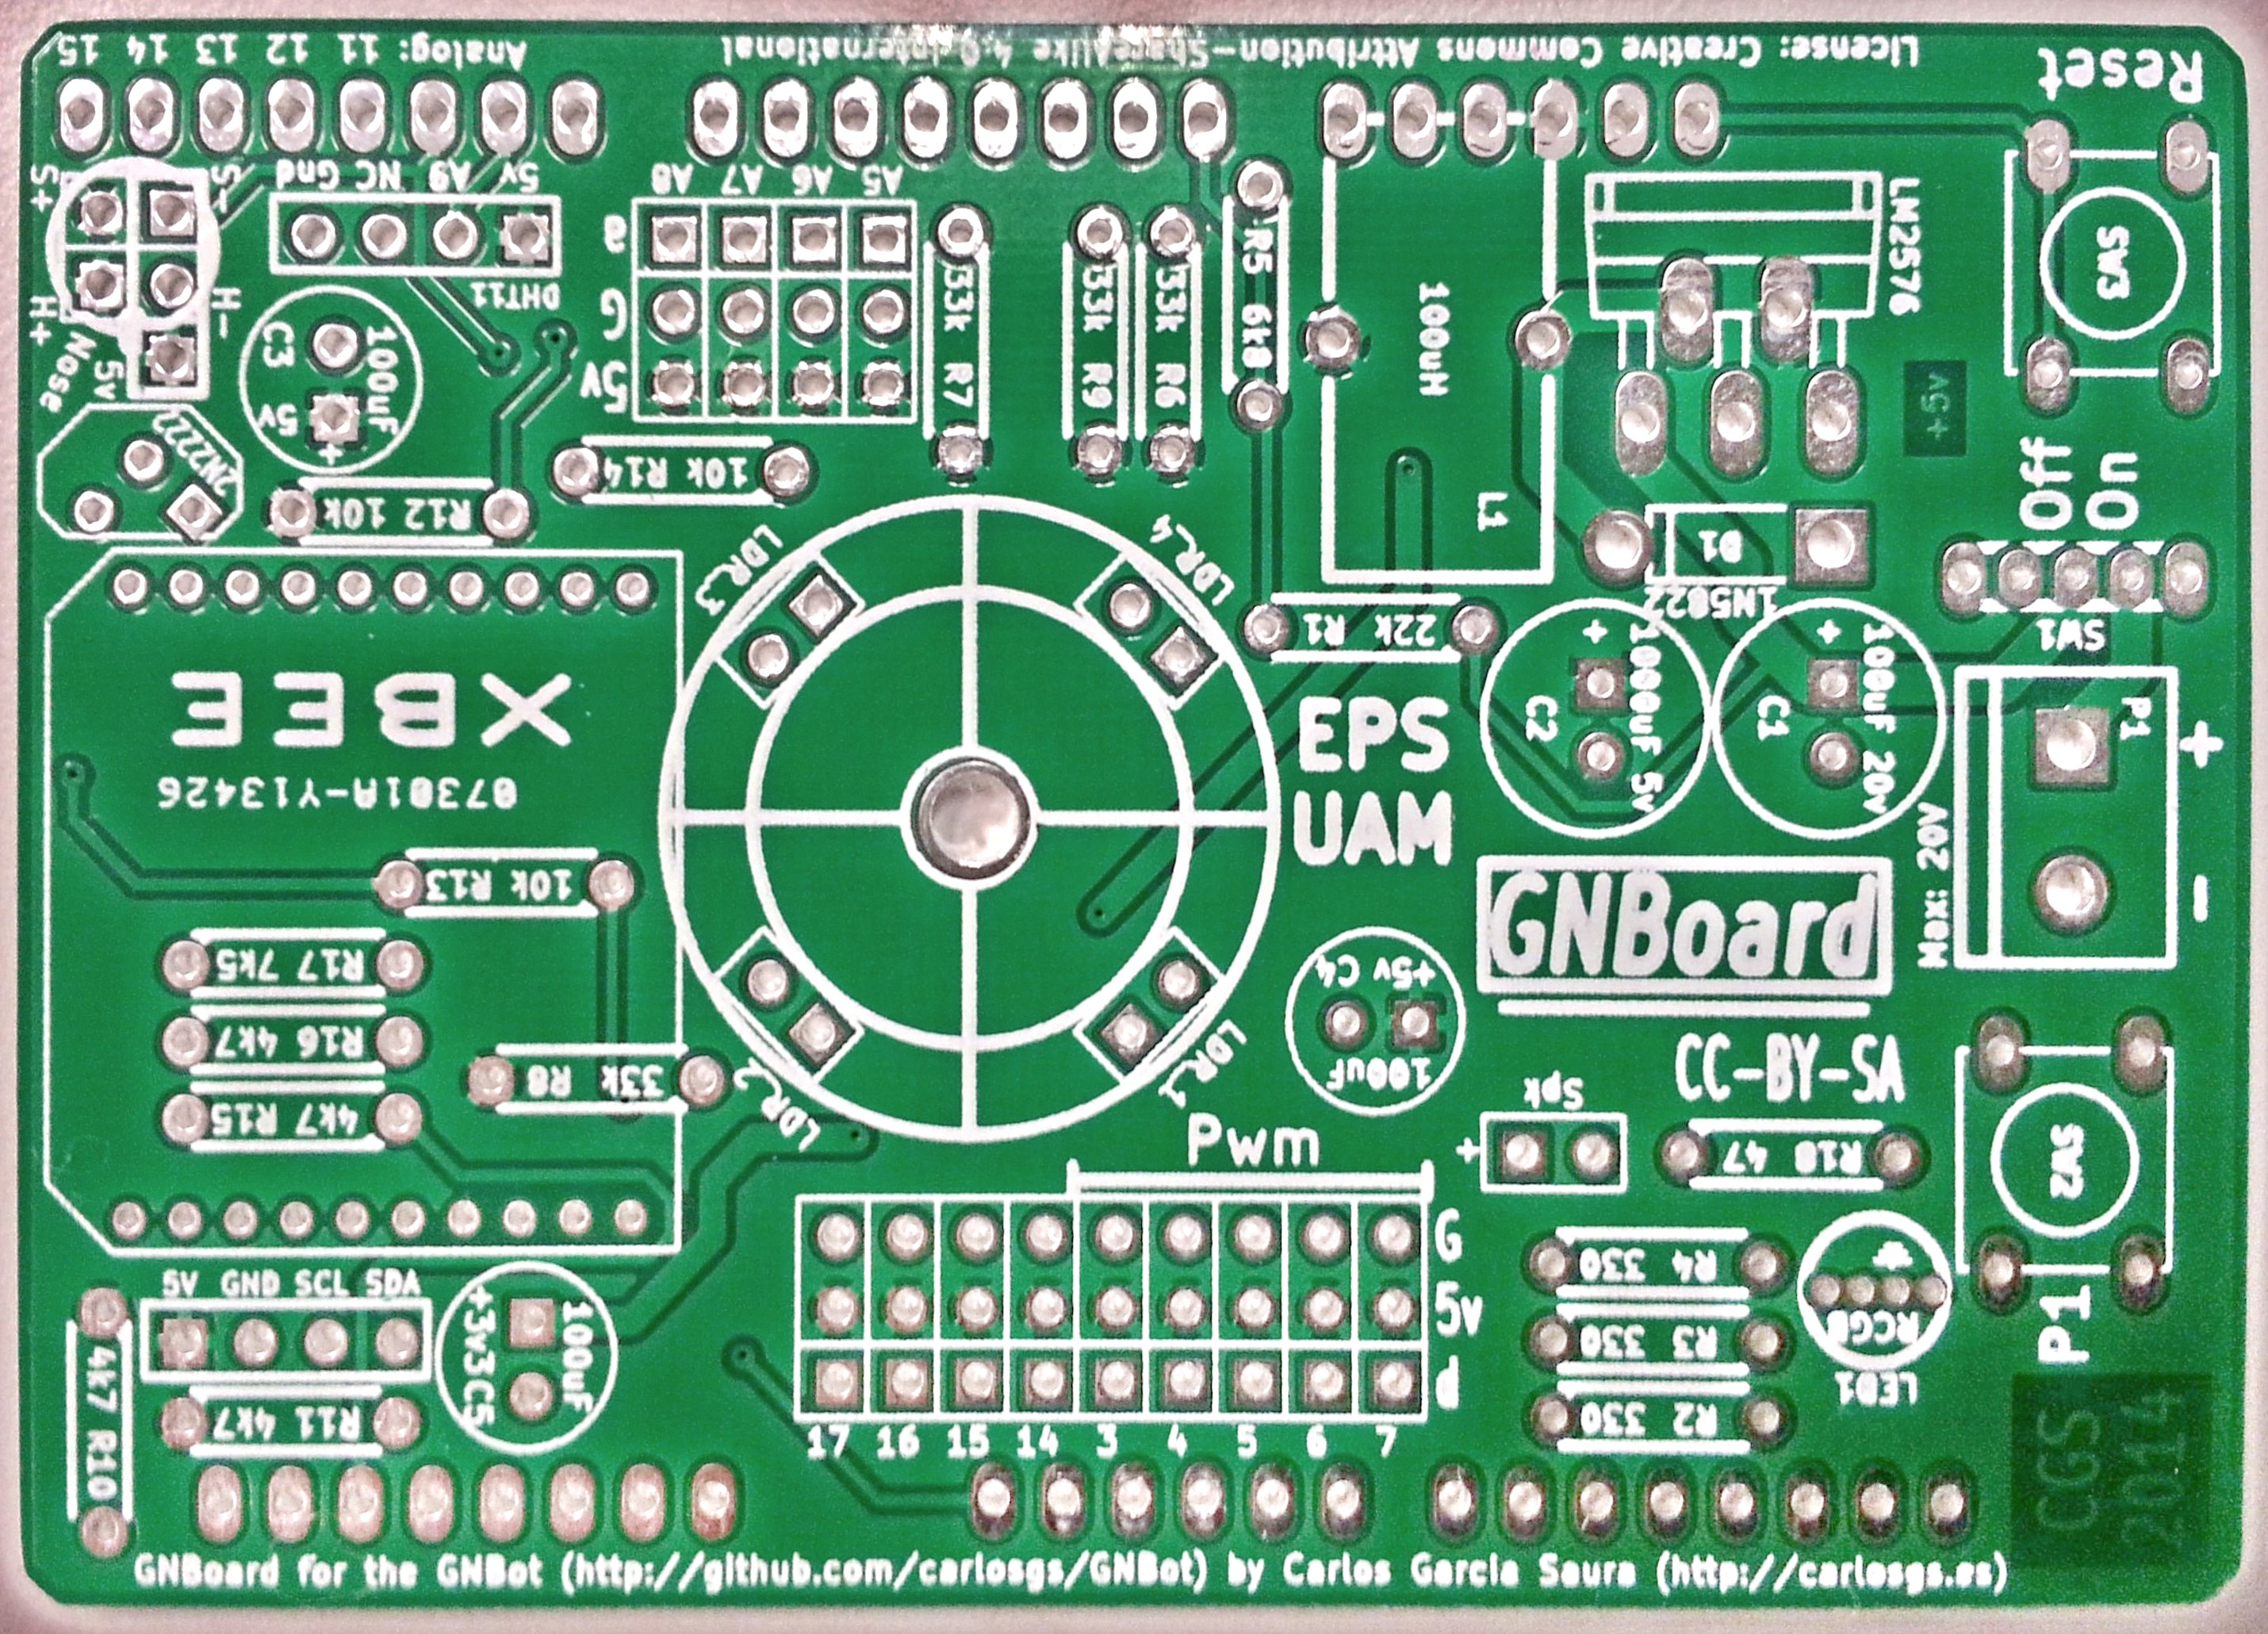
\includegraphics[width=11cm]{images/gnboard_pcb_real.jpg}}}
\captionFigure{Manufactured PCB for the GNBoard v1.0}
{fig:gnboard_pcb_real}{
A total of 20 boards were ordered to \url{http://www.seeedstudio.com/}. The layout utilizes through-hole components solely, in order to simplify the assembly task.
}
\end{figure}




\newpage
%\thispagestyle{empty}
\begin{figure}[h!]
\centerline{\mbox{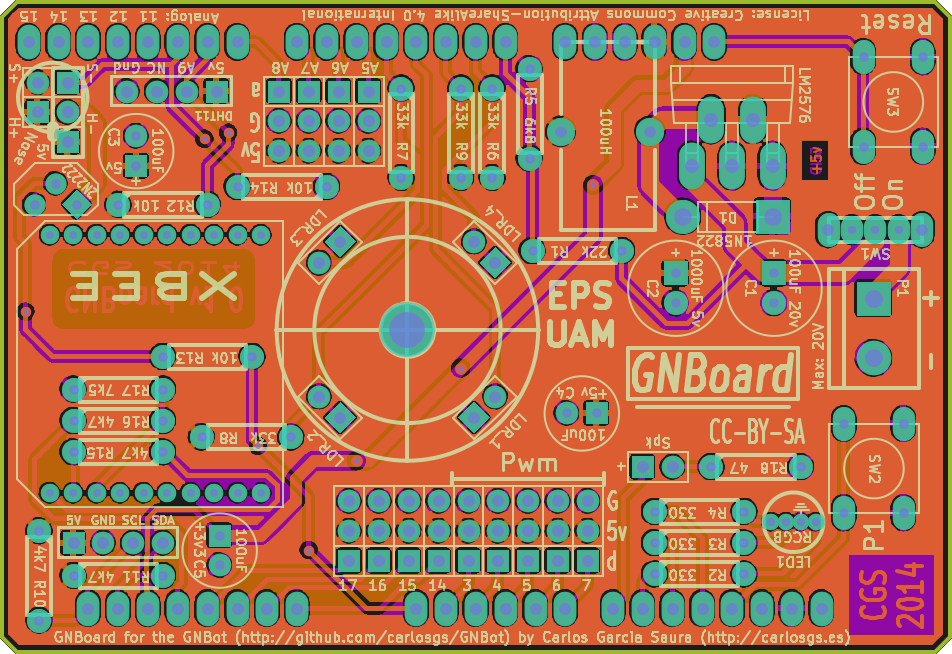
\includegraphics[width=13.5cm]{images/GNBoard_top.png}}}
\vspace{0.5cm}
\centerline{\mbox{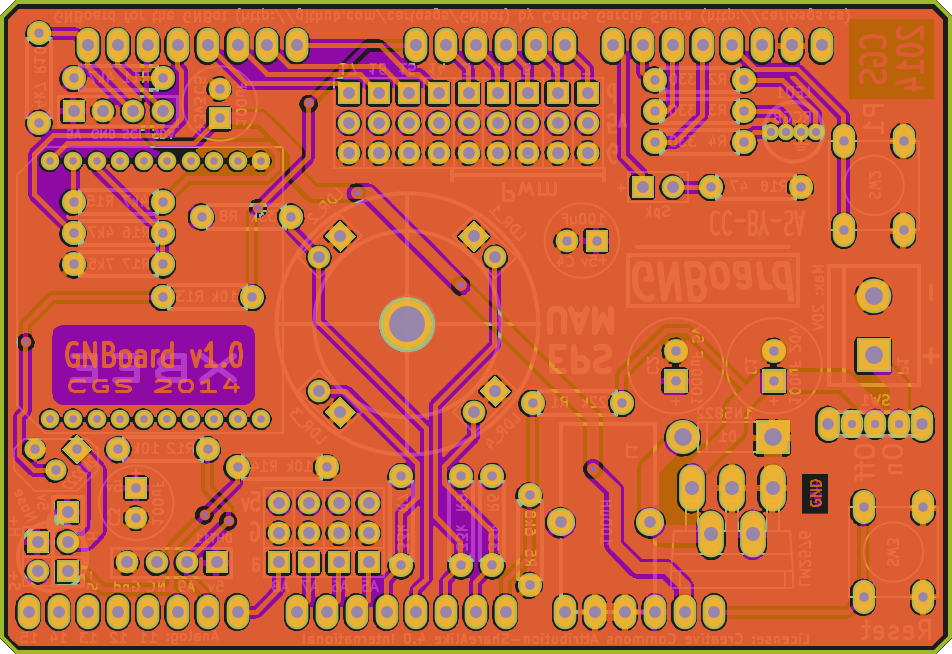
\includegraphics[width=13.5cm]{images/GNBoard_btm.png}}}
\centering\captionFigure{GNBoard v1.0 layout}
{fig:GNBoard_layout}{
Top and bottom views.\\
More information can be found in Section \ref{sect:openSourceElectronics}.
}
\end{figure}





\newpage
\thispagestyle{empty}

\newgeometry{top=3.5cm,bottom=4.5cm,left=1cm,right=0cm}

\begin{landscape}

\begin{figure*}[tb] 
\centering
 \makebox[\textwidth]{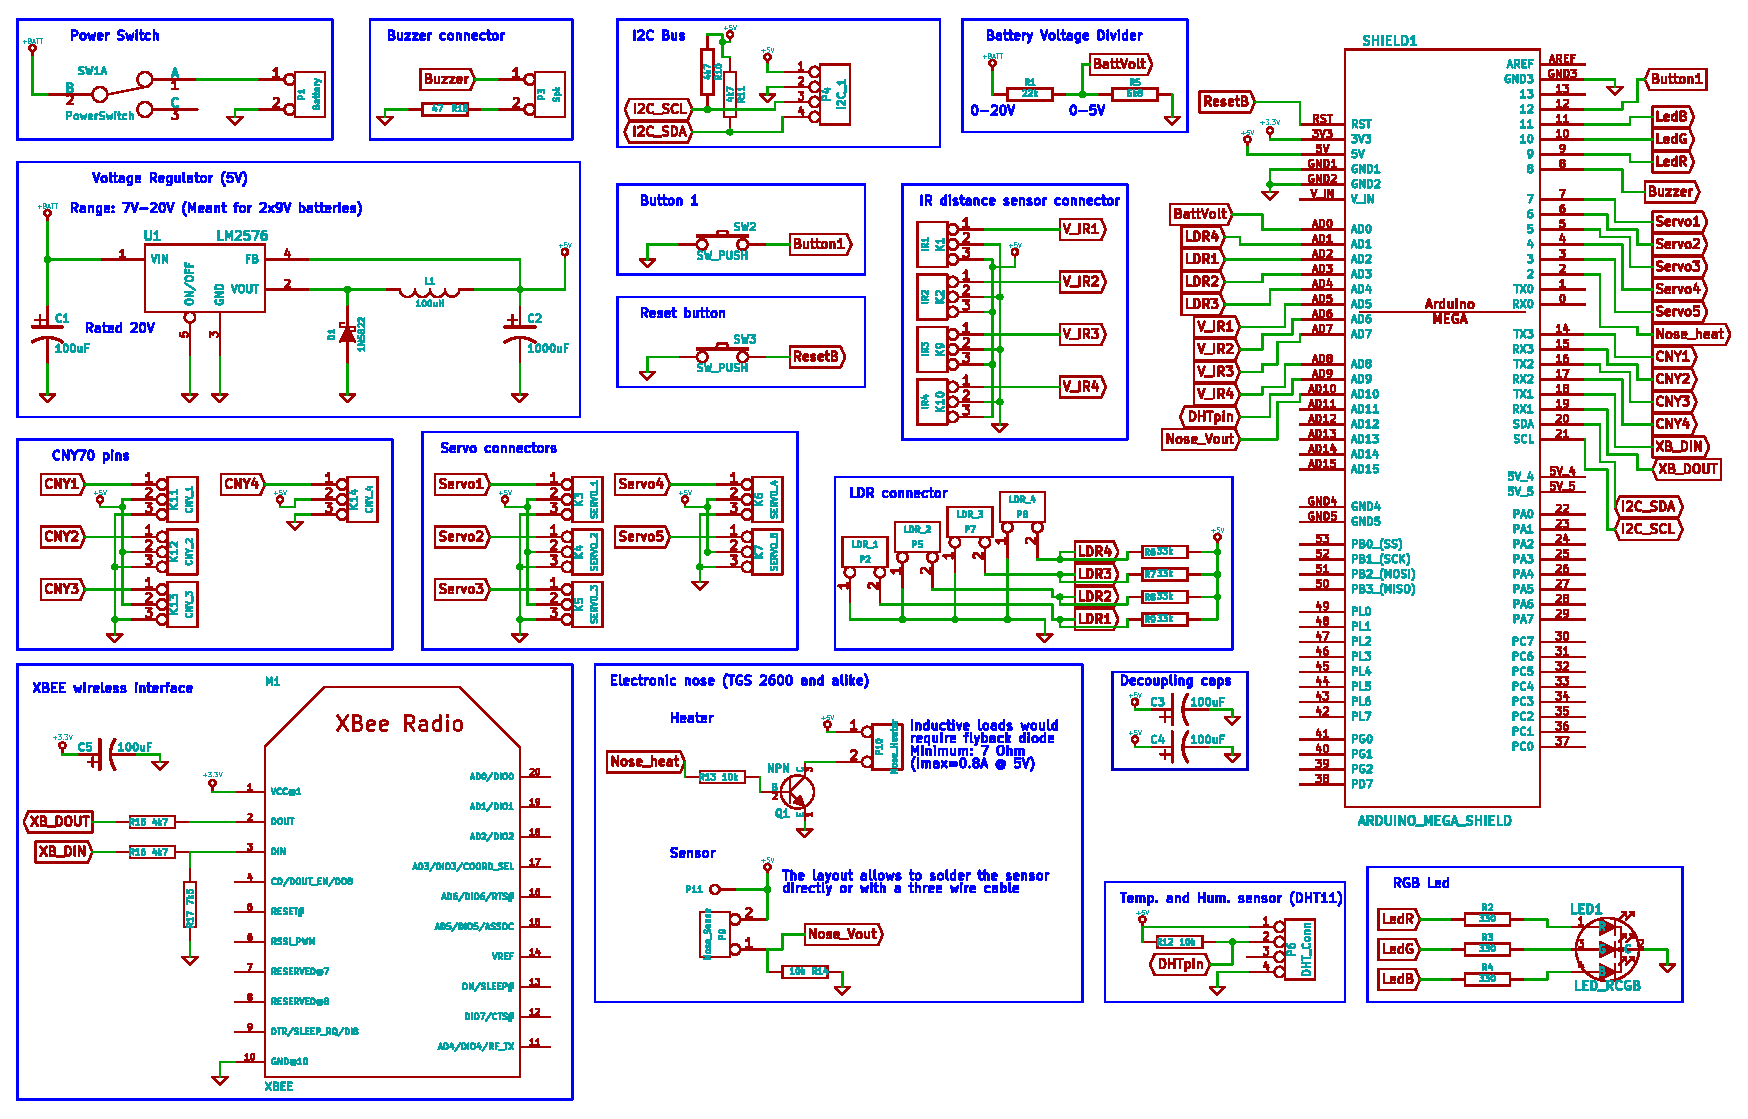
\includegraphics[width=.9\paperheight]{images/GNBoard_schem.eps}}
\captionFigure{GNBoard v1.0 schematic}
{fig:GNBoard_schem}{
More information can be found in Section \ref{sect:openSourceElectronics}.
}
\end{figure*}

\end{landscape}

\restoregeometry

\newpage \thispagestyle{empty} % Página vacía 




\chapter{Publications}
\label{Appendix:designStrategies}
\vspace{-1cm}

This work resulted in the following paper to be presented July 30th at Living Machines 2014\footnote{\url{http://csnetwork.eu/livingmachines/conf2014}} \emph{(3rd International Conference on Biomimetic and Biohybrid Systems)} in Milan, and published in \emph{Springer Lecture Notes in Artificial Intelligence} series:

\textbf{Carlos Garc\'{i}a-Saura, Francisco de Borja Rodr\'{i}guez, and Pablo Varona. ``Design Principles for Cooperative Robots with Uncertainty-Aware and Resource-Wise Adaptive Behavior''. Living Machines 2014, LNAI 8608, pp. 108-117, 2014.}

A spanish version of the article, entitled ``Dise\~{n}o de una plataforma rob\'{o}tica para la implementaci\'{o}n de algoritmos de b\'{u}squeda cooperativa de fuentes de olor'', has been presented to the \emph{Arquimedes National Research Contest}\footnote{\url{https://sede.educacion.gob.es/catalogo-tramites/becas-ayudas-subvenciones/premios/premios-estudiantes/certamen-arquimedes/certamen-arquimedes-2014.html}} in May 2014.


\newpage \thispagestyle{empty} % P�gina vac�a 


%Hoja final en blanco
\newpage \thispagestyle{empty} % Página vacía

\end{document}
